\documentclass[twocolumn,10pt]{article}

\usepackage[a4paper,margin=2cm]{geometry}
\usepackage{graphicx}
\usepackage{amsmath}
\usepackage{amssymb}
\usepackage{xcolor}
\usepackage{booktabs}
\usepackage{subcaption}
\usepackage{lineno}
\captionsetup{font=small,skip=6pt}
\usepackage[colorlinks=true,allcolors=blue]{hyperref}

% This TeX tree lacks the TS1 (text-companion) metrics for Computer Modern and
% cannot render Latin Modern Type1 fonts, so redirect any TS1 request to the
% classic CM roman that is present. We emit no genuine TS1 glyphs, so this only
% suppresses spurious font-loading errors.
\DeclareFontFamily{TS1}{cmr}{}
\DeclareFontShape{TS1}{cmr}{m}{n}{<-> cmr10}{}
\DeclareFontShape{TS1}{cmr}{m}{it}{<-> cmti10}{}
\DeclareFontShape{TS1}{cmr}{bx}{n}{<-> cmbx10}{}

% Draw itemize markers from the available Computer Modern math-symbol font.
\renewcommand{\labelitemi}{\ensuremath{\bullet}}

% --- float placement / vertical spacing (layout only) ---
% Let floats occupy more of a page and avoid near-empty float pages, and stop
% the two-column default (\flushbottom) from stretching sparse columns with
% large inter-paragraph gaps.
\renewcommand{\topfraction}{0.92}
\renewcommand{\bottomfraction}{0.85}
\renewcommand{\textfraction}{0.07}
\renewcommand{\floatpagefraction}{0.75}
\renewcommand{\dbltopfraction}{0.95}
\renewcommand{\dblfloatpagefraction}{0.72}
\setcounter{topnumber}{3}
\setcounter{bottomnumber}{2}
\setcounter{totalnumber}{4}
\setcounter{dbltopnumber}{3}
% Pack float-only pages from the top instead of stretching the gaps.
\makeatletter
\setlength{\@fptop}{0pt}
\setlength{\@fpsep}{12pt}
\setlength{\@dblfptop}{0pt}
\setlength{\@dblfpsep}{12pt}
\makeatother
% Keep float-to-text gaps compact without squeezing captions or plot labels.
\setlength{\textfloatsep}{12pt plus 2pt minus 2pt}
\setlength{\dbltextfloatsep}{12pt plus 2pt minus 2pt}
\setlength{\floatsep}{10pt plus 2pt minus 2pt}
\setlength{\dblfloatsep}{10pt plus 2pt minus 2pt}
\raggedbottom

% --- lightweight siunitx replacement (siunitx not installed here) ---
% \SI{value}{unit} -> value + thin space + unit, works in text and math.
\providecommand{\SI}[2]{\mbox{#1\,#2}}
\providecommand{\num}[1]{\mbox{#1}}
\pdfstringdefDisableCommands{\def\SI#1#2{#1 #2}}

% --- convenience macros (consistent notation across the paper) ---
\newcommand{\R}{\ensuremath{R}}                 % displacement radius
\newcommand{\alphainc}{\ensuremath{\alpha}}     % non-pointing / incidence angle
\newcommand{\dc}{\ensuremath{d_{c}}}            % CLUE density radius
\newcommand{\rhoc}{\ensuremath{\rho_{c}}}       % CLUE seed density
\newcommand{\dm}{\ensuremath{d_{m}}}            % CLUE max distance to higher
\newcommand{\dxy}{\ensuremath{d_{XY}}}          % projective transverse distance
\newcommand{\clue}{CLUE}
\newcommand{\cluethreed}{CLUE3D}
\newcommand{\cluestering}{CLUEstering}

\title{\vspace{-2em}\bfseries Reconstruction of long-lived particles\\ with the CLUE algorithm in CMS}
\author{Frane Doljanin\\
  \small\textit{CERN Summer Student Programme}\\
  \small\href{mailto:fdoljanin@pmfst.hr}{\texttt{fdoljanin@pmfst.hr}}\\[0.4em]
  \small\textit{Supervisor: Bruno Alves, CERN, Experimental Physics Department}\\
  \small\href{mailto:bruno.alves@cern.ch}{\texttt{bruno.alves@cern.ch}}}
\date{September 11, 2026}

\begin{document}
\linenumbers

% Full-width title + abstract across both columns
\twocolumn[
  \begin{@twocolumnfalse}
    \maketitle
    \begin{abstract}
      \noindent
      The CMS experiment at the LHC is upgrading its endcap
calorimeters with the High-Granularity Calorimeter (HGCAL). Long-lived particles can decay far from the
interaction point and produce photons whose trajectories do not point back to
it. Reconstructing these photons is a challenge for \cluethreed{}, the
clustering algorithm developed for HGCAL.

This project studies \cluethreed{} performance using simulated single- and
two-photon events, with and without pileup. We improved the displaced-photon
generator and added displacement observables to the standard validation tools.
The results show that \cluethreed{} loses efficiency as displacement increases,
with single showers fragmenting and nearby showers becoming mixed. Adding pileup
leaves the signal-photon efficiency largely unchanged. Tests of the alternative
\cluestering{} algorithm show that suitable configurations improve
displaced-photon reconstruction while keeping nearby showers separate. Further
tuning and tests with realistic long-lived-particle decays are needed.

    \end{abstract}
    \vspace{1.5em}
  \end{@twocolumnfalse}
]

\section{Introduction}
\label{sec:intro}

The year 2030 will mark the start of the High-Luminosity phase of the Large
Hadron Collider (HL-LHC)~\cite{HLLHC}, which will deliver proton--proton
collisions at an unprecedented luminosity. The resulting data
volume and the severe pileup---of order $200$ simultaneous interactions per
bunch crossing---demand a new generation of reconstruction algorithms. To cope
with these conditions the CMS experiment will replace its endcap calorimeters
with the High-Granularity Calorimeter (HGCAL)~\cite{HGCALTDR}, a sampling
calorimeter with roughly six million channels arranged in about fifty
longitudinal layers. Its fine transverse and longitudinal segmentation capture detailed three-dimensional structure of electromagnetic and hadronic
showers. It also makes traditional calorimeter clustering impractical and
motivates dedicated clustering algorithms.

\begin{figure*}[!tp]
  \centering
  \begin{subfigure}[b]{0.38\textwidth}
    \centering
    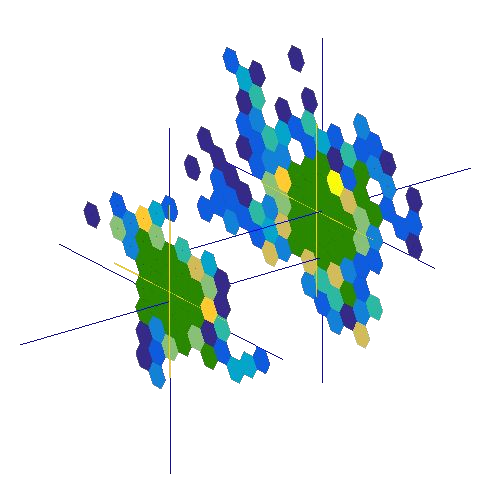
\includegraphics[height=4.6cm,keepaspectratio]{figures/VISUAL_rechits.png}
    \caption{RecHits and LayerClusters}
    \label{fig:rechits-a}
  \end{subfigure}
  \hspace{0.04\textwidth}
  \begin{subfigure}[b]{0.56\textwidth}
    \centering
    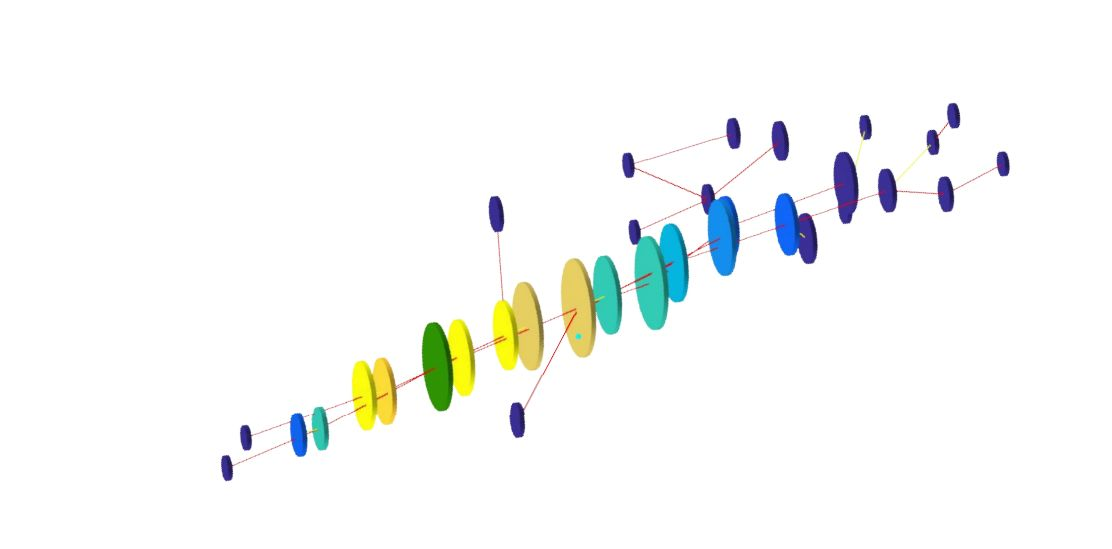
\includegraphics[height=4.6cm,keepaspectratio]{figures/VISUAL_tracks.jpg}
    \caption{LayerClusters linked into a Trackster}
    \label{fig:rechits-b}
  \end{subfigure}
  \caption{The HGCAL reconstruction chain. (a) Calibrated energy deposits
  (RecHits) of two photon showers. CLUE groups them by layer into
  two-dimensional LayerClusters.
  (b) \cluethreed{} links LayerClusters across layers into a
  three-dimensional Trackster; the red lines are the nearest-higher links that
  build the shower.}
  \label{fig:rechits}
\end{figure*}

The Clustering of Energy (CLUE) algorithm~\cite{Rovere2020clue} was developed for this purpose: it is a fast, parallel, energy density-based clustering algorithm. It groups HGCAL energy deposits into physics objects such as photons and
electrons. In the CMS reconstruction, CLUE and its three-dimensional extension
\cluethreed{} sit inside The Iterative Clustering (TICL)
framework~\cite{TICL}, which builds objects in stages
(Fig.~\ref{fig:rechits}): individual calorimeter hits (\emph{RecHits}) are first
grouped per layer by CLUE into two-dimensional \emph{LayerClusters} (LCs);
\cluethreed{} then links LayerClusters from multiple layers into three-dimensional
\emph{Tracksters}; and a subsequent linking step associates Tracksters into the
final TICL candidates. The Monte Carlo truth is described by an analogous chain,
in which a generated particle (\emph{CaloParticle}) is mapped to a
\emph{SimTrackster} that collects the LayerClusters that belong to it.
Reconstruction performance is measured by comparing reconstructed Tracksters to
SimTracksters through their shared energy.

An important \cluethreed{} assumption: the neighbour search that links layer
clusters across layers is performed in a coordinate system projected from
the interaction point (IP), therefore shower travelling outward
from the CMS centre keeps fixed projected position layer to layer. This
holds for \emph{prompt} particles produced at the beamline, but it doesn't need to for
the class of \emph{long-lived particles} (LLPs) predicted by many extensions of
the Standard Model~\cite{LLPreview}. Rather than decaying within a few
millimetres of IP, an LLP can travel longer distance in the detector before decaying, producing \emph{displaced}, non-pointing
particles. A representative signature is a dark shower in which
long-lived dark hadrons decay to Standard Model photons far from the beamline. Because these showers do not point back to
the origin, they may violate exactly the assumption on which \cluethreed{}
relies.

The goal of this project is to determine
is \cluethreed{} capable of clustering the energy deposits from such
novel topologies, to measure the expected performance degradation as a function
of the distance from IP to where LLP decays, and to explore an alternative algorithm. We restrict the study to
neutral \emph{photons}: photons whose trajectory is not curved by the CMS magnetic field, so
they go in straight lines and their displacement is unambiguously defined; they also do not interact in the tracker before
reaching the calorimeter. This isolates the calorimeter clustering behaviour
from tracking and magnetic-field effects and provides the cleanest possible test
of the origin assumption.

The remainder of this report is organized as follows. We first define the
displacement observables and describe how they are defined for reconstructed objects, then present the displaced-photon Monte Carlo
production and the performance metrics. After reviewing how \cluethreed{} works,
with emphasis on the origin assumption, we present the single-photon efficiency,
the two-shower merging behaviour, and the performance under pileup, before
comparing \cluethreed{} against the alternative algorithm \cluestering{} and
concluding.

\section{Displacement observables}
\label{sec:displacement}

Every result in this report is expressed as a function of \emph{how displaced}
a shower is. We therefore begin by defining the displacement observables and,
crucially, by explaining how they are obtained for reconstructed objects that
carry no truth information.

\subsection{Definitions}

\begin{figure}[!htbp]
  \centering
  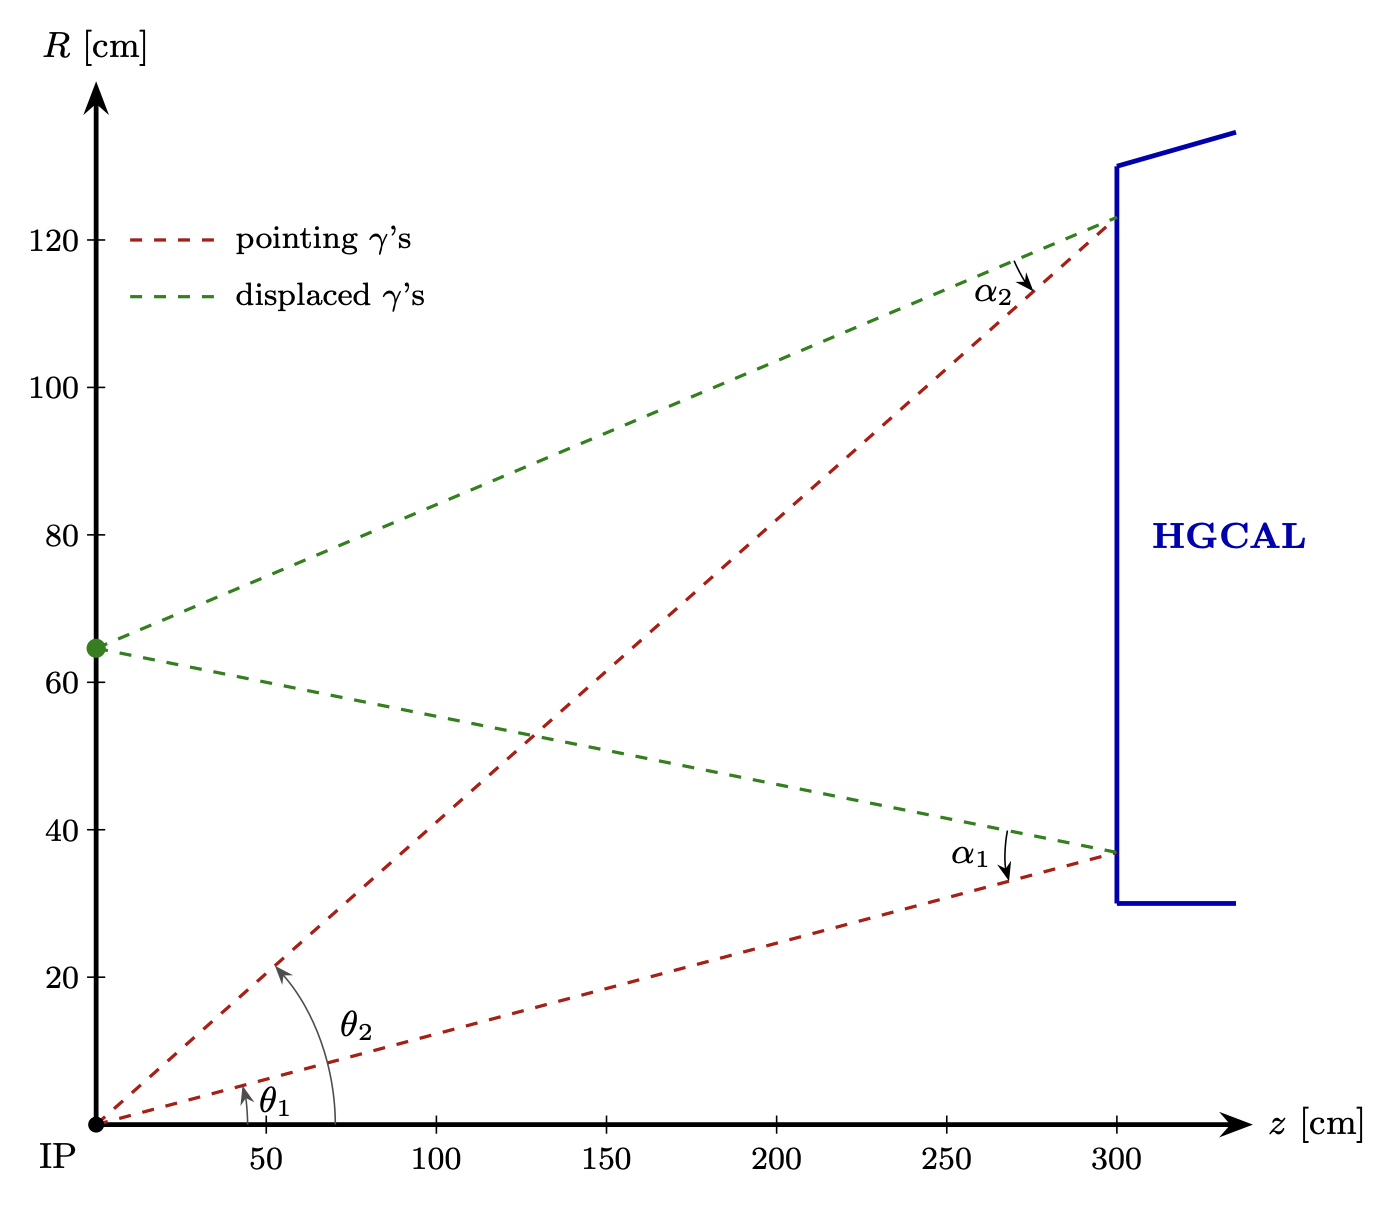
\includegraphics[width=\linewidth]{figures/hgcal_nonpointing.png}
  \caption{Displacement geometry in the $(z,R)$ plane. Pointing photons (red)
  travel radially from the interaction point (IP) and reach the HGCAL front face
  at a polar angle $\theta$ with non-pointing angle $\alphainc=0$. Displaced
  photons (green) originate at a transverse distance $\R$ from the beamline at
  $z=0$ and strike the calorimeter with $\alphainc>0$; two displaced trajectories
  from the same vertex illustrate that a single $\R$ can correspond to different
  incidence angles $\alphainc$.}
  \label{fig:geometry}
\end{figure}

Consider a photon that is created at a production vertex
$\mathbf{x}_v=(x_v,y_v,z_v)$ and travels in a straight line to the HGCAL front
face, located at $z\simeq\SI{321}{cm}$ from the interaction
point (Fig.~\ref{fig:geometry}). We characterize its displacement by two
quantities:
\begin{itemize}
  \item the \textbf{displacement radius} \R{}, defined as the transverse
  distance from the beamline at which the photon's extrapolated trajectory crosses the plane
  $z=0$,
  \begin{equation}
    \R = \sqrt{x_0^2 + y_0^2}\,,
    \label{eq:Rdef}
  \end{equation}
  where $(x_0,y_0)$ is the trajectory back-projected to $z=0$;
  \item the \textbf{non-pointing angle} \alphainc{}, the angle between the
  photon's momentum $\mathbf{p}$ and its position vector at the HGCAL face,
  i.e.\ the line joining the interaction point to the impact point
  $\mathbf{x}_{\text{face}}$,
  \begin{equation}
    \alphainc = \arccos\!\left(
      \frac{\mathbf{x}_{\text{face}}\cdot\mathbf{p}}
           {\lvert\mathbf{x}_{\text{face}}\rvert\,\lvert\mathbf{p}\rvert}
    \right).
    \label{eq:alphadef}
  \end{equation}
  A prompt, pointing photon travels radially, so
  $\mathbf{x}_{\text{hit}}\parallel\mathbf{p}$ and $\R=\alphainc=0$; a displaced
  photon has $\R>0$ and $\alphainc>0$.
\end{itemize}
It is also useful to introduce the polar angle $\theta$ between the photon
momentum and the beam axis, with $\tan\theta = p_T/|p_z|$. As shown in
Fig.~\ref{fig:geometry}, \alphainc{} rather than \R{} is the more fundamental driver of the clustering
behaviour, but \R{} has a direct geometric interpretation as the transverse distance, so both are retained throughout.

For a \emph{simulated} photon these quantities are trivial: the production
vertex and momentum are known from the generator, and \R{} follows from a
straight-line extrapolation. We verified this extrapolation numerically---the
displacement computed from the SimTrackster's SimTrack reproduces the generator-level value, and pointing photons correctly yield
$\R,\alphainc\approx0$.

\subsection{Reconstructing the displacement}

The difficulty lies on the reconstruction side. A reconstructed Trackster has no
production vertex, and it does not need to correspond one-to-one to a SimTrackster: it
may contain only a fragment of a true shower, or it may span multiple showers.
Nonetheless, the fake-, duplicate- and merge-rate metrics defined below require a
displacement value in order to place each Trackster in a histogram bin. We therefore reconstruct \R{} directly from the
Trackster geometry.

Each Trackster provides an energy-weighted barycentre
$\mathbf{x}_c=(x_c,y_c,z_c)$ and a principal-axis direction
$\mathbf{u}=(u_x,u_y,u_z)$ obtained from a principal-component analysis (PCA) of
its LayerClusters. Treating the shower as a straight line through
$\mathbf{x}_c$ along $\mathbf{u}$ and extrapolating to $z=0$ gives
\begin{align}
  x_0 &= x_c - z_c\,\frac{u_x}{u_z}\,, &
  y_0 &= y_c - z_c\,\frac{u_y}{u_z}\,,
  \label{eq:recoR}
\end{align}
and $\R_{\text{reco}}=\sqrt{x_0^2+y_0^2}$ from Eq.~\eqref{eq:Rdef}. Care is taken so that the extrapolation uses the
correct sign of $u_z$. This straight-line treatment is exact for photons, which
makes them the ideal probe for validating the method.

\subsection{Error budget and the choice of direction estimator}

\begin{figure*}[!tp]
  \centering
  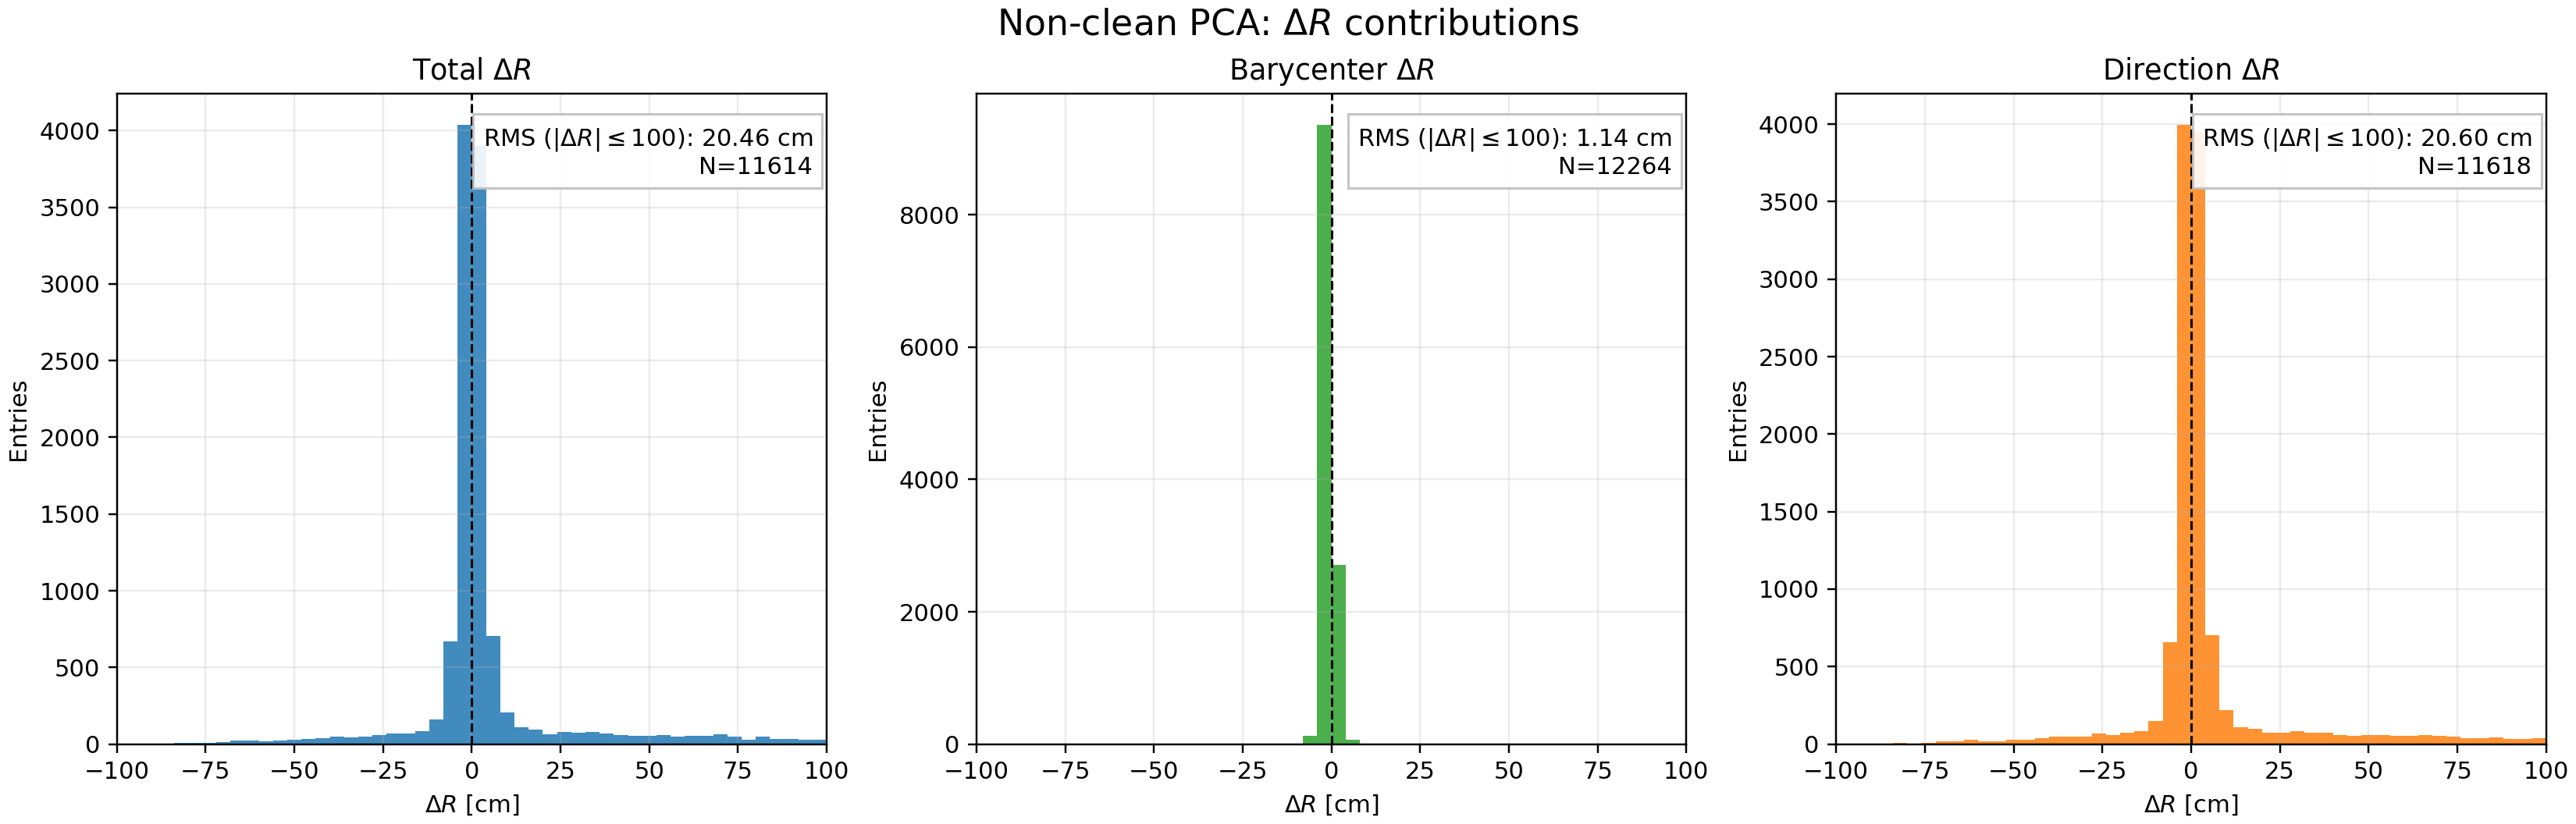
\includegraphics[width=0.88\textwidth]{figures/non_clean_pca_deltaR_contributions.png}
  \caption{Decomposition of the displacement-radius error into its two sources,
  for the default (ordinary) PCA. \emph{Left:} the full error
  $\Delta\R=\R_{\text{reco}}-\R_{\text{truth}}$
  ($\text{RMS}=\SI{20.46}{cm}$). \emph{Centre:} the error when only the
  barycentre is reconstructed and the true direction is used
  ($\text{RMS}=\SI{1.14}{cm}$). \emph{Right:} the error when only the direction
  is reconstructed and the true barycentre is used
  ($\text{RMS}=\SI{20.60}{cm}$). The direction term alone reproduces the full
  error, proving that the resolution budget is spent almost entirely on the
  shower direction.}
  \label{fig:decomp}
\end{figure*}

The accuracy of $\R_{\text{reco}}$ sets the resolution with which any reco-side
metric can be studied, so we characterized its error in detail. We quantify it by
\begin{equation}
  \Delta\R \equiv \R_{\text{reco}} - \R_{\text{truth}},
  \label{eq:deltaR}
\end{equation}
summarized throughout by its RMS. Our starting point was the direction estimator
that CMSSW already exposes: the ordinary PCA of \texttt{TrackstersPCA.cc}, which
builds the energy-weighted covariance matrix of the LayerCluster positions about
the barycentre, and makes the shower direction $\mathbf{u}$ to be its leading
eigenvector (the axis of largest spatial variance). Reusing this default out of
the box gave a broad error---$\text{RMS}(\Delta\R)\approx\SI{20}{cm}$ for the
sample of Fig.~\ref{fig:decomp}---and before trying to improve it we wanted to
know \emph{where} that error came from.

The error has only two possible sources, the barycentre $\mathbf{x}_c$ and the
direction $\mathbf{u}$, and they can be separated cleanly. We recompute
$\Delta\R$ twice: once with the reconstructed barycentre but the \emph{true}
direction (isolating the barycentre error), and once with the true barycentre but
the reconstructed direction (isolating the direction error). The answer is unambiguous (Fig.~\ref{fig:decomp}): the
barycentre alone contributes only $\text{RMS}(\Delta\R)=\SI{1.14}{cm}$, whereas
the direction alone contributes $\SI{20.60}{cm}$ and by itself reproduces the
$\SI{20.46}{cm}$ of the full error. The barycentre is essentially
perfect; the direction is entirely to blame. The reason is geometric: the
barycentre sits inside the shower and is well measured, but the small angular
uncertainty of $\mathbf{u}$ is amplified by the long
$z_c\sim\SI{320}{cm}$ over which Eq.~\eqref{eq:recoR} extrapolates back to $z=0$.
The same figure shows a systematic positive bias of order $+\SI{3}{cm}$,
consistent with \R{} being a positive-definite quantity.

Having localized the problem to the direction, we implemented and compared
several estimators of the shower axis. Each takes the LayerClusters (or RecHits)
of a Trackster and returns a unit direction:
\begin{itemize}
  \item \textbf{Ordinary PCA} (the CMSSW default): leading eigenvector of the
  energy-weighted covariance matrix
  $C=\sum_i w_i(\mathbf{x}_i-\mathbf{x}_c)(\mathbf{x}_i-\mathbf{x}_c)^{\!\top}$,
  where $\mathbf{x}_i$ and $w_i$ are the position and energy of LayerCluster $i$.
  It uses every LayerCluster, so secondary per-layer clusters and stray fragments
  can tilt the axis.
  \item \textbf{Clean PCA (10-to-10)}: the same eigenvector computation, but on a
  cleaned set that keeps only the single highest-energy LayerCluster in each
  layer, restricted to the ten layers before and the ten layers after the
  peak-energy layer. This suppresses the off-axis fragments that bias the
  covariance while retaining the well-measured shower core.
  \item \textbf{Endpoint layers}: the direction joining the barycentre of the
  first populated layer of the window to that of the last. It uses only the two
  extremes, so it is simple but sensitive to endpoint fluctuations.
  \item \textbf{Window barycentres}: per-layer energy-weighted barycentres are
  formed across the window and their trend in $z$ defines the axis, averaging out
  single-layer noise.
  \item \textbf{Weighted straight-line fit}: the shower is parametrized as a line
  $x(z)=x_0+(u_x/u_z)\,z$, $y(z)=y_0+(u_y/u_z)\,z$, and the slopes are obtained by
  minimizing the energy-weighted sum of squared transverse residuals of the
  LayerClusters to that line---a direct least-squares alternative to the PCA.
  \item \textbf{Weighted line fit with outlier refit}: the same fit, after which
  the $20\%$ of LayerClusters with the largest residuals are discarded and the
  line is refitted, reducing the pull of outliers; we tried this both on the
  $10$-to-$10$ window and over all layers.
  \item \textbf{RecHit PCA}: the covariance-eigenvector method applied to the raw
  RecHits instead of the LayerClusters, testing whether the finer granularity
  below the LayerCluster level helps.
\end{itemize}

\begin{figure*}[!tp]
  \centering
  \begin{subfigure}[t]{0.49\textwidth}
    \centering
    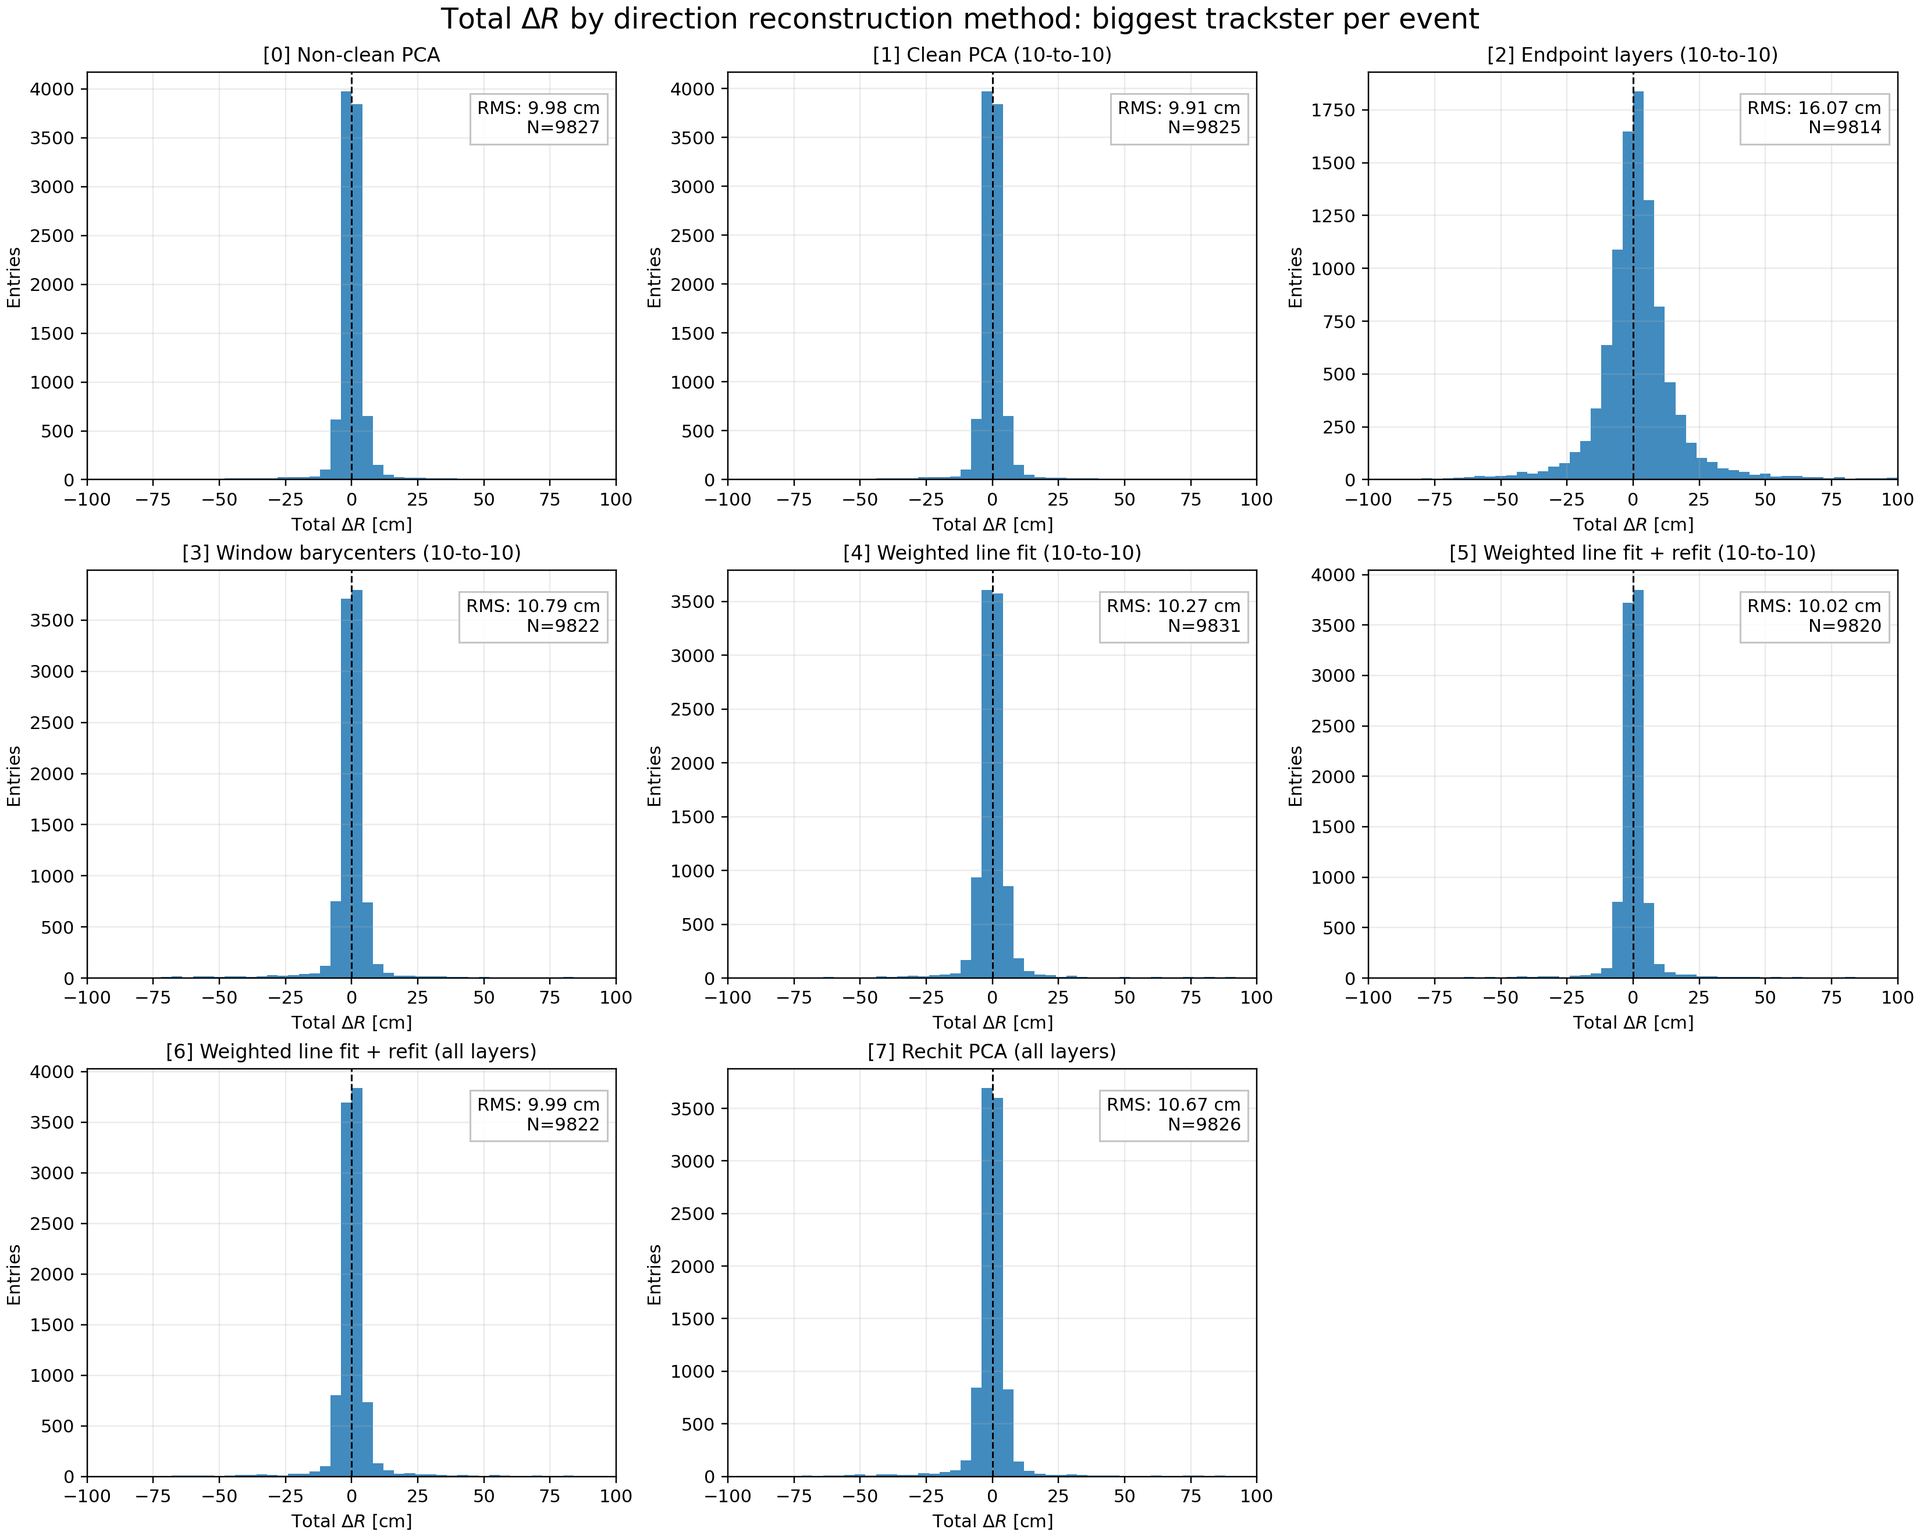
\includegraphics[width=\linewidth]{figures/r_resolution_methods_leading.png}
    \caption{leading (most energetic) Trackster per event}
    \label{fig:methods-lead}
  \end{subfigure}
  \hfill
  \begin{subfigure}[t]{0.49\textwidth}
    \centering
    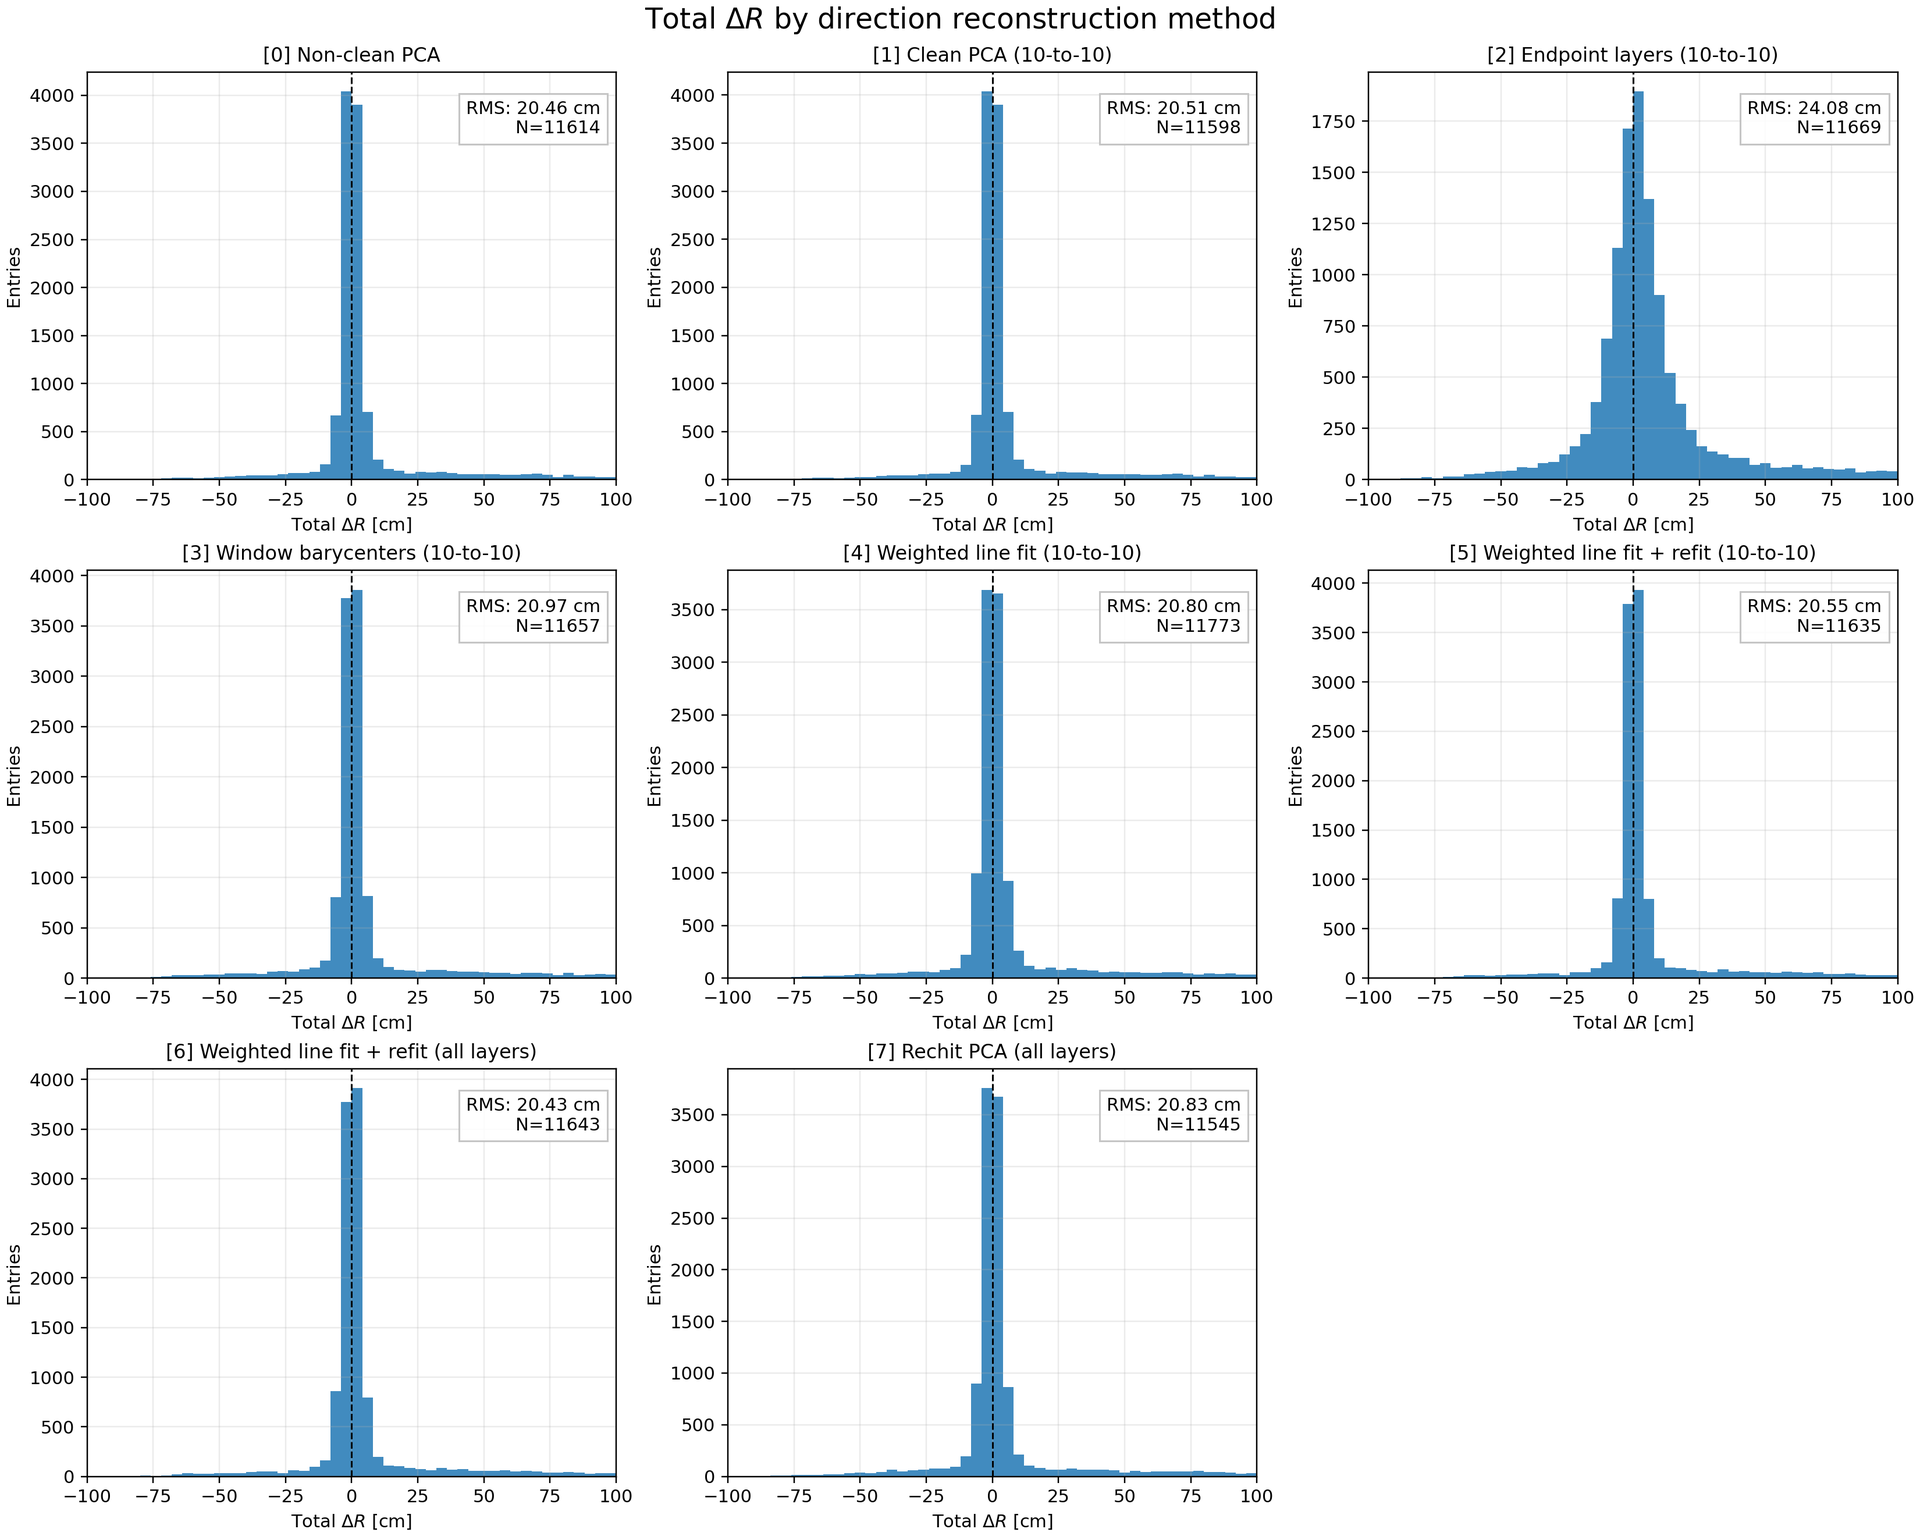
\includegraphics[width=\linewidth]{figures/method_grid_all_tracksters.png}
    \caption{all Tracksters in the event}
    \label{fig:methods-all}
  \end{subfigure}
  \caption{Full-error distribution $\Delta\R$ for each of the eight direction
  estimators, (a) restricting to the leading Trackster and (b) over all
  Tracksters. Restricting to the leading Trackster, the PCA variants are the
  narrowest (clean PCA \SI{9.91}{cm}, ordinary \SI{9.98}{cm}) and the endpoint
  estimate the broadest (\SI{16.07}{cm}). Over all Tracksters every estimator
  instead collapses to $\sim\SI{20}{cm}$. The choice of estimator barely
  matters, because the sample is then dominated by low-energy fragments whose
  direction no method can fit.}
  \label{fig:methods}
\end{figure*}

The comparison (Fig.~\ref{fig:methods}) makes clear that no estimator
improves decisively on the default. On the leading Trackster (most energetic one per event, closest to the truth) the PCA variants are
already the best and the more elaborate line fits merely match them; over all
Tracksters (which includes small fragments) every method collapses to the same $\sim\SI{20}{cm}$, so the estimator
is almost irrelevant and it is the Trackster selection that drives the
resolution. Because the clean PCA is both robust and already implemented in
CMSSW, it was adopted as the default.

\begin{figure*}[!tp]
  \centering
  \begin{subfigure}[b]{0.49\textwidth}
    \centering
    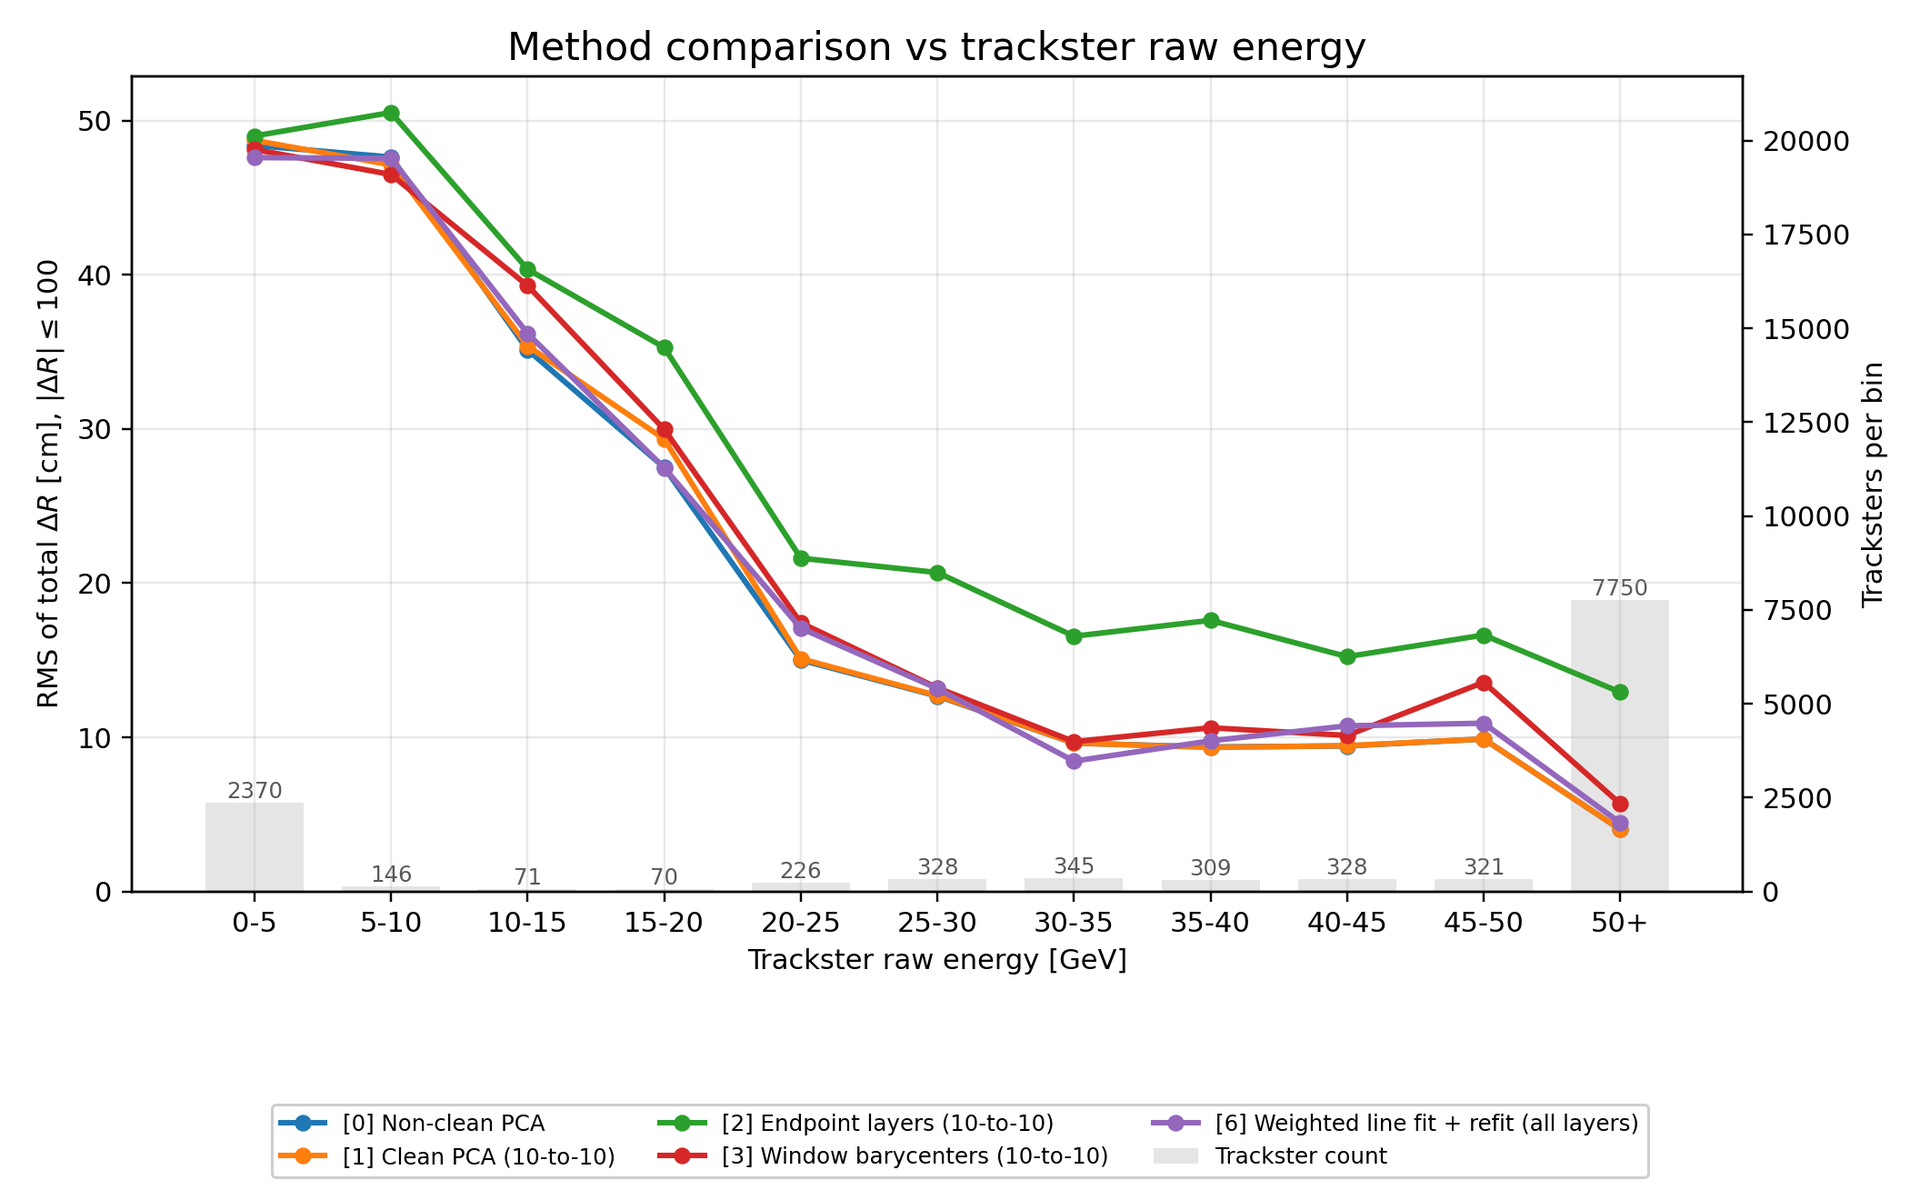
\includegraphics[width=\linewidth]{figures/r_resolution_vs_energy.png}
    \caption{versus Trackster raw energy}
    \label{fig:restrend-e}
  \end{subfigure}
  \hfill
  \begin{subfigure}[b]{0.49\textwidth}
    \centering
    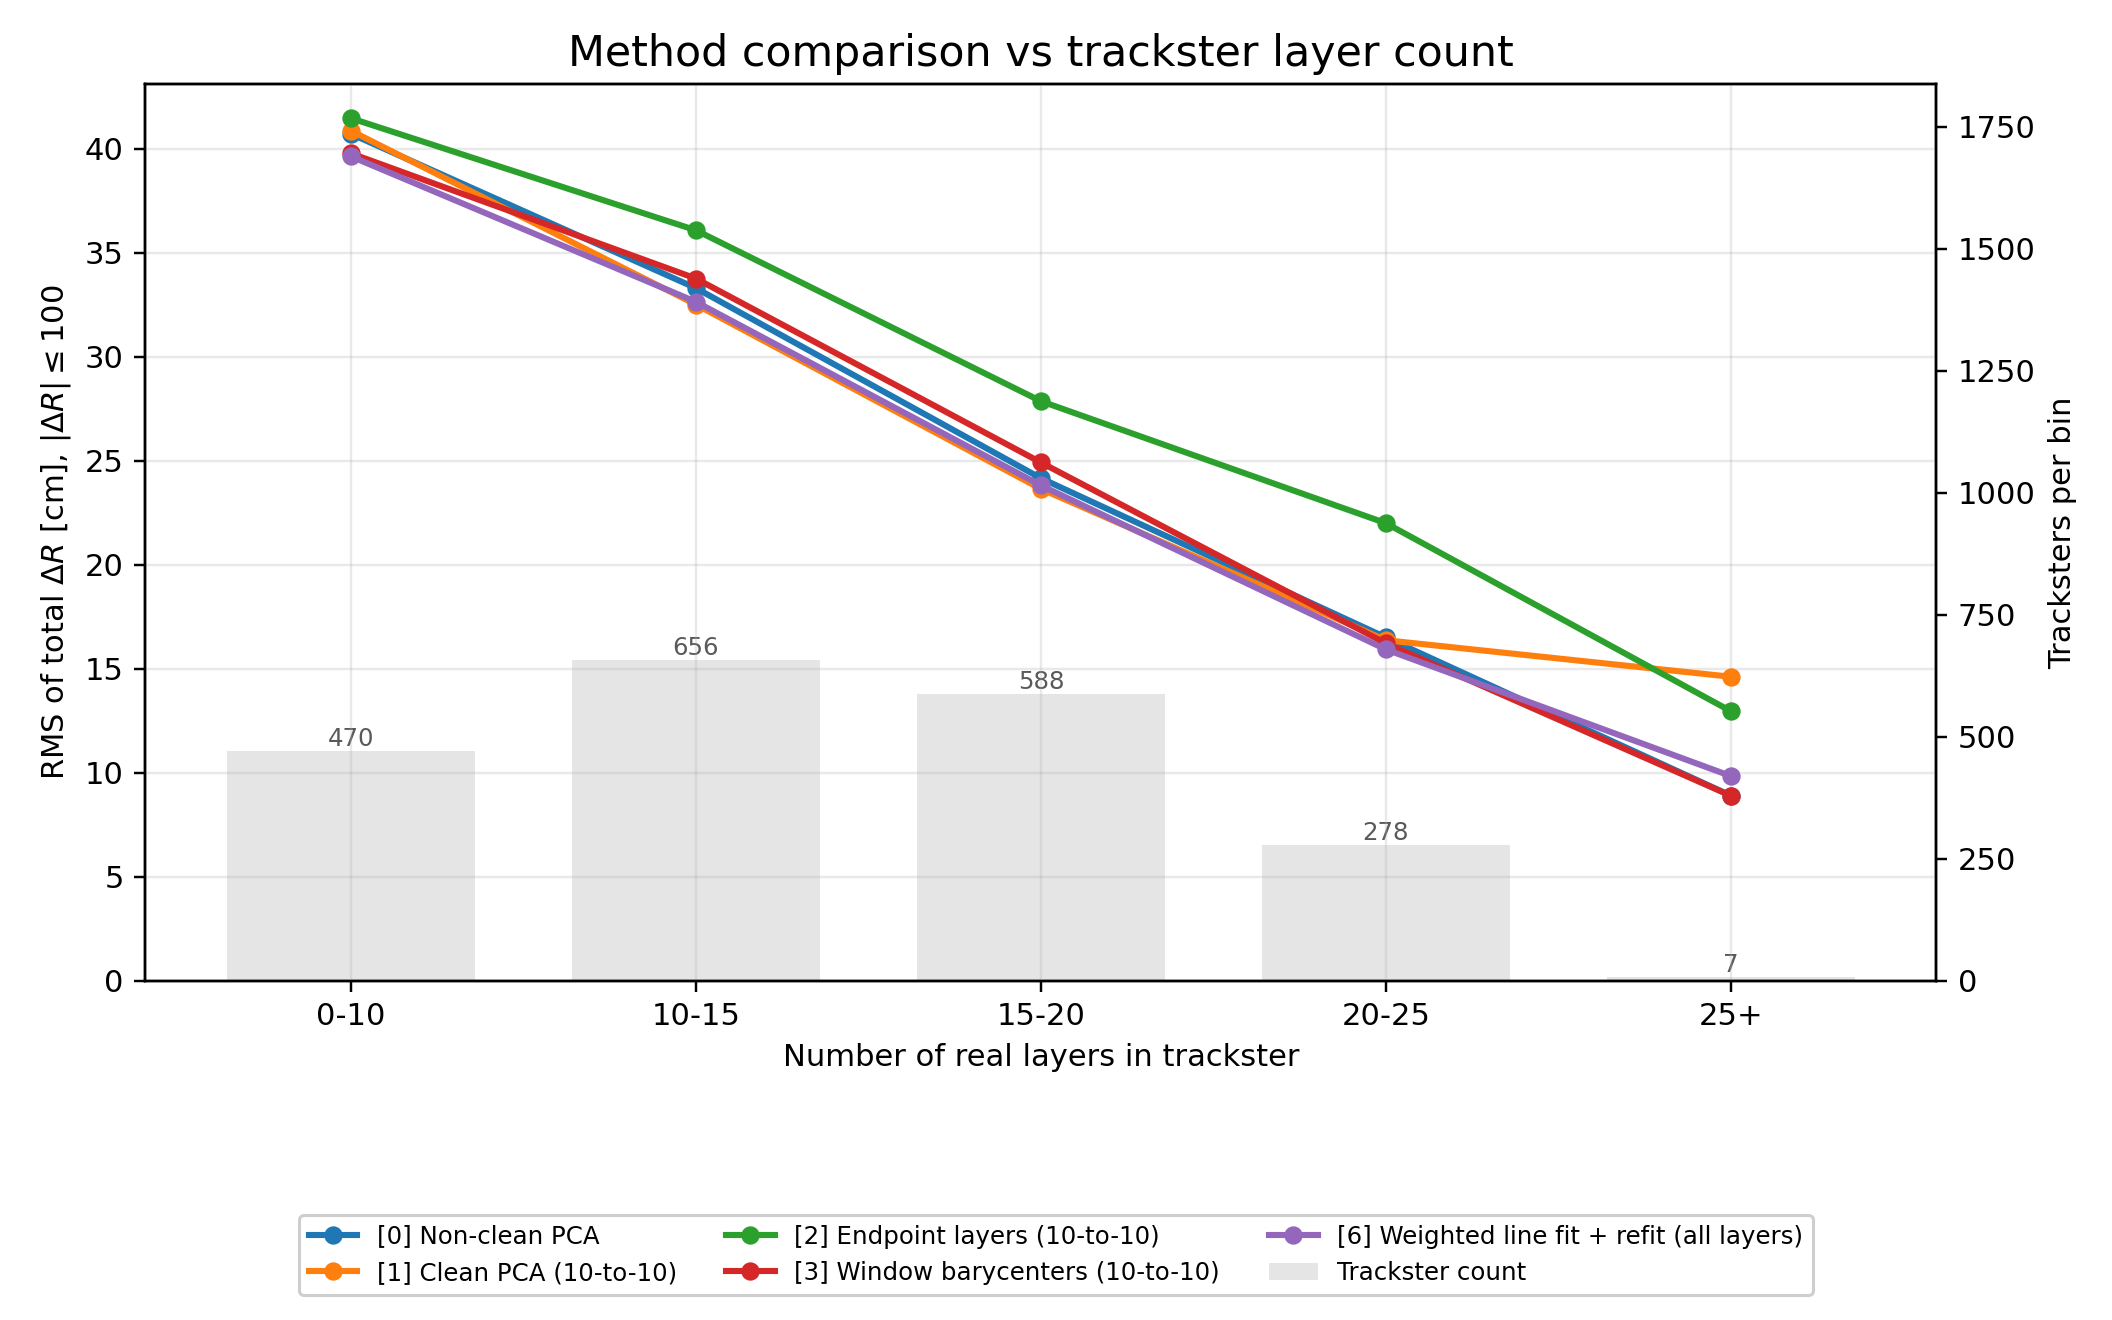
\includegraphics[width=\linewidth]{figures/method_resolution_vs_layer_count.png}
    \caption{versus number of layers}
    \label{fig:restrend-l}
  \end{subfigure}
  \caption{Displacement-radius resolution $\text{RMS}(\Delta\R)$ versus
  (a) Trackster raw energy and (b) the number of layers the Trackster spans, for
  each estimator (coloured curves). The resolution improves by a factor of
  several from low to high energy and from few to many layers, confirming that
  the error tracks how well the shower direction can be fitted. Grey bars (right
  axis) give the Trackster count per bin.}
  \label{fig:restrend}
\end{figure*}

This picture is confirmed by binning the resolution in Trackster observables
(Fig.~\ref{fig:restrend}): the RMS falls from
$\sim\SI{48}{cm}$ below \SI{10}{GeV} to $\sim\SI{10}{cm}$ above \SI{25}{GeV}, and
from $\sim\SI{40}{cm}$ below ten layers to $\lesssim\SI{10}{cm}$ beyond twenty,
with the layer count the cleanest single predictor. The error is thus worst
exactly where the axis is hardest to fit---sparse, low-energy Tracksters spanning
few layers---which is why selecting the single most energetic Trackster per
event, the object that actually carries the photon, is what brings the clean
$10$-to-$10$ PCA to $\text{RMS}(\Delta\R)=\SI{9.91}{cm}$.

We judged this $\sim\SI{10}{cm}$ leading-Trackster resolution good enough to bin
every reconstruction-side metric that follows, and chose the clean $10$-to-$10$
PCA to compute \R{}. A natural next step, left outside the scope of this project,
would be to add a further dimension to the direction fit: each LayerCluster also
carries a timing measurement, and a displaced, non-pointing shower arrives with a
time-of-flight pattern that constrains its direction independently of the spatial
axis. Exploiting Trackster timing to sharpen $\R_{\text{reco}}$ is a promising
avenue for future work.

The displacement observables \R{} and \alphainc{}, together with a
Trackster-timing observable, were added to the standard HGCAL validation as new
per-object quantities so that any efficiency, purity, duplicate or merge plot
can be produced as a function of displacement (CMSSW pull request
\href{https://github.com/cms-sw/cmssw/pull/51510}{\#51510}).

\section{Displaced photon gun}
\label{sec:gun}

To measure the dependence of reconstruction performance on displacement, we
need samples in which the shower energy and trajectory can be controlled
independently of a particular LLP model. For this purpose, Bruno Alves developed
the original displaced-particle gun for the project (CMSSW pull request
\href{https://github.com/cms-sw/cmssw/pull/51006}{\#51006}). My contribution was
to test and improve this generator: I revised its sampling and
configuration, corrected the production timing, and updated the beamspot choice
in the generation workflow. These improvements are collected in pull request
\href{https://github.com/cms-sw/cmssw/pull/51489}{\#51489}.

The studies use photons, whose trajectories are not bent by the magnetic field.
The photons are inserted into the simulation immediately before HGCAL, so they
do not traverse the tracker and convert or shower there. This isolates the response to calorimeter for a non-pointing photon. The gun therefore supplies a
controlled test of the reconstruction geometry; it does not simulate the full
production and decay of an LLP.

\subsection{Trajectory geometry and surface constraints}

The construction distinguishes the \emph{sampled origin} from the actual
\emph{production vertex} passed to the detector simulation. The origin is a
point in the plane $z=0$,
\begin{equation}
  \mathbf{x}_0=(\R\cos\phi_0,\R\sin\phi_0,0),
\end{equation}
so its radius is exactly the displacement observable defined in
Section~\ref{sec:displacement}. Given a momentum polar angle $\theta$ and
azimuth $\phi_p$, the straight trajectory is
\begin{equation}
  \mathbf{x}_{\perp}(z)=\mathbf{x}_{0,\perp}
    +z\tan\theta\,(\cos\phi_p,\sin\phi_p).
  \label{eq:gunline}
\end{equation}
Here $\theta$ is measured from the positive beam axis, while $\phi_0$ specifies
the position of the origin and $\phi_p$ specifies the momentum direction. These
two azimuths do not need to coincide. The non-pointing angle $\alphainc$ follows from
the resulting trajectory and impact point; it is not independently sampled.

The photon is created where this line crosses a configurable
\emph{production plane}, placed at $z=\SI{319}{cm}$ in the example
configuration. Its position must lie within a specified annulus, optionally
restricted in azimuth. An additional \emph{target plane}, near the back of the
electromagnetic calorimeter at $z\simeq\SI{362}{cm}$, can impose a second
annular acceptance. Requiring the line to pass through both regions selects
trajectories that enter the calorimeter and continue through its volume. Suitable radial margins can reduce edge leakage, although an accepted
trajectory alone does not guarantee containment of the entire shower, whose
transverse spread is set by the calorimeter's Moli\`ere radius. The
target constraint is optional and assumes straight propagation, so the
implementation permits it only for neutral particles.

In particular, neither surface is a second independently sampled vertex. Both
constrain the same line from $\mathbf{x}_0$, and the production vertex is
obtained by evaluating Eq.~\eqref{eq:gunline} at the production-plane position.
Consequently, back-extrapolating the generated momentum from that vertex
recovers the sampled $\R$, even though the photon is actually introduced into
the simulation far downstream of $z=0$.

\subsection{Sampling without biasing the displacement scan}

The improved gun supports two distributions for the origin radius. Sampling
$\R^2$ uniformly gives a constant density per unit transverse area, with
$\mathrm{d}N/\mathrm{d}\R\propto\R$. Sampling $\R$ uniformly instead gives
equal expected populations in equal-width displacement bins. We use the latter
for displacement scans. The origin azimuth is sampled uniformly within its
configured range.

A simple approach would draw a direction and discard the entire trial whenever
it misses either surface. This can be inefficient and, if the origin is also
redrawn, changes the accepted displacement distribution according to the
geometric acceptance. The improved implementation holds the sampled origin fixed
and constructs the allowed polar-angle intervals before drawing $\theta$.
For a trial momentum azimuth $\phi_p$, write $s=\tan\theta$. At a surface
$z=z_k$, the squared transverse radius is
\begin{equation}
  r_k^2(s)=\R^2+2z_k\R\cos(\phi_p-\phi_0)s+z_k^2s^2.
  \label{eq:gunconstraint}
\end{equation}
The annular requirement
$r_{k,\min}^2\leq r_k^2(s)\leq r_{k,\max}^2$ gives allowed intervals in
$s$. The gun intersects these intervals for the production plane, the optional
target plane, and the configured $\theta$ bounds. It then samples uniformly in
$\theta$ over the surviving intervals, weighting each interval by its angular
width.

Momentum azimuths with no allowed interval are retried. Spatial azimuthal cuts
on the surfaces are checked after sampling and can also reject a direction.
The origin remains fixed throughout: exhausting the configurable attempt limit
raises an error instead of silently replacing an inconvenient origin. Geometry
checks also reject some incompatible configurations before generation begins.
This preserves the requested origin distribution in a successfully generated
sample while avoiding many impossible direction trials. It does not imply that
the accepted impact positions or the overall $\theta$ distribution are uniform;
both reflect the surface constraints.

The momentum magnitude is sampled after a valid trajectory has been found. The
configuration explicitly selects either a uniform total-energy distribution or
a uniform transverse-momentum distribution, together with the corresponding
range. For photons these choices are related by
\begin{equation}
  E=\frac{p_T}{\sin\theta},
  \label{eq:gunenergy}
\end{equation}
in units with $c=1$. Thus, a fixed $p_T$ range produces increasingly energetic
photons at small $\theta$. Sampling $E$ directly allows the energy distribution
to be held independent of the accepted direction, which is useful when
isolating displacement effects.

\begin{figure*}[!tp]
  \centering
  \begin{subfigure}[t]{0.49\textwidth}
    \centering
    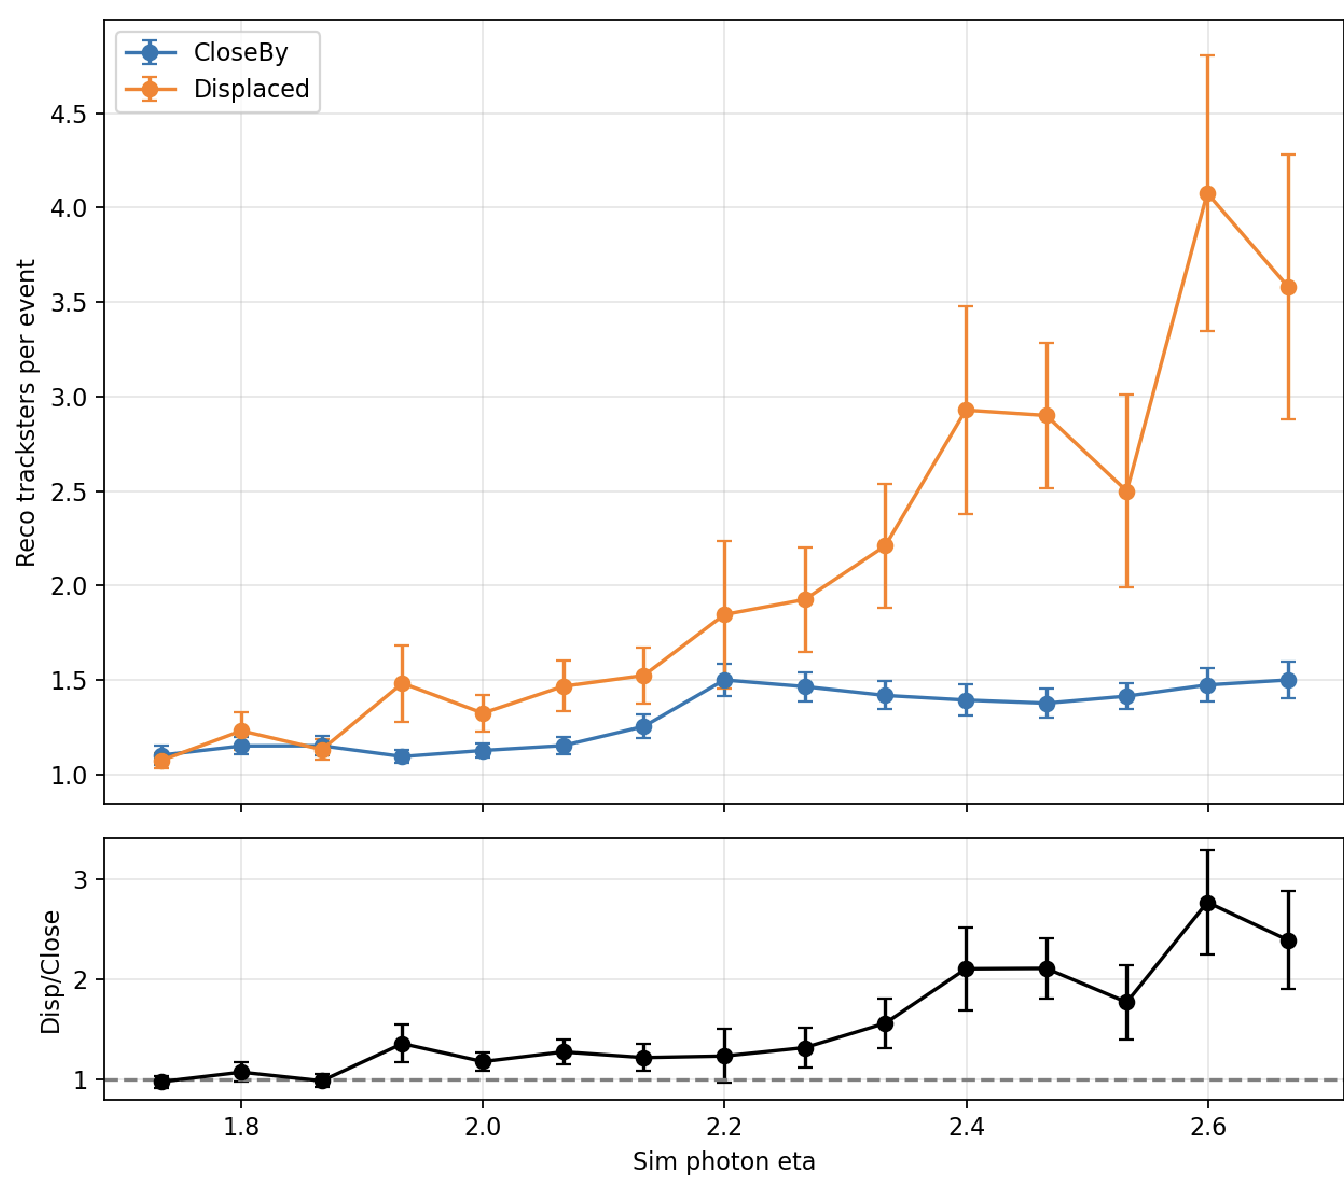
\includegraphics[width=\linewidth]{figures/gun_comparison_pt.png}
    \caption{Displaced gun sampling $p_T$}
  \end{subfigure}
  \hfill
  \begin{subfigure}[t]{0.49\textwidth}
    \centering
    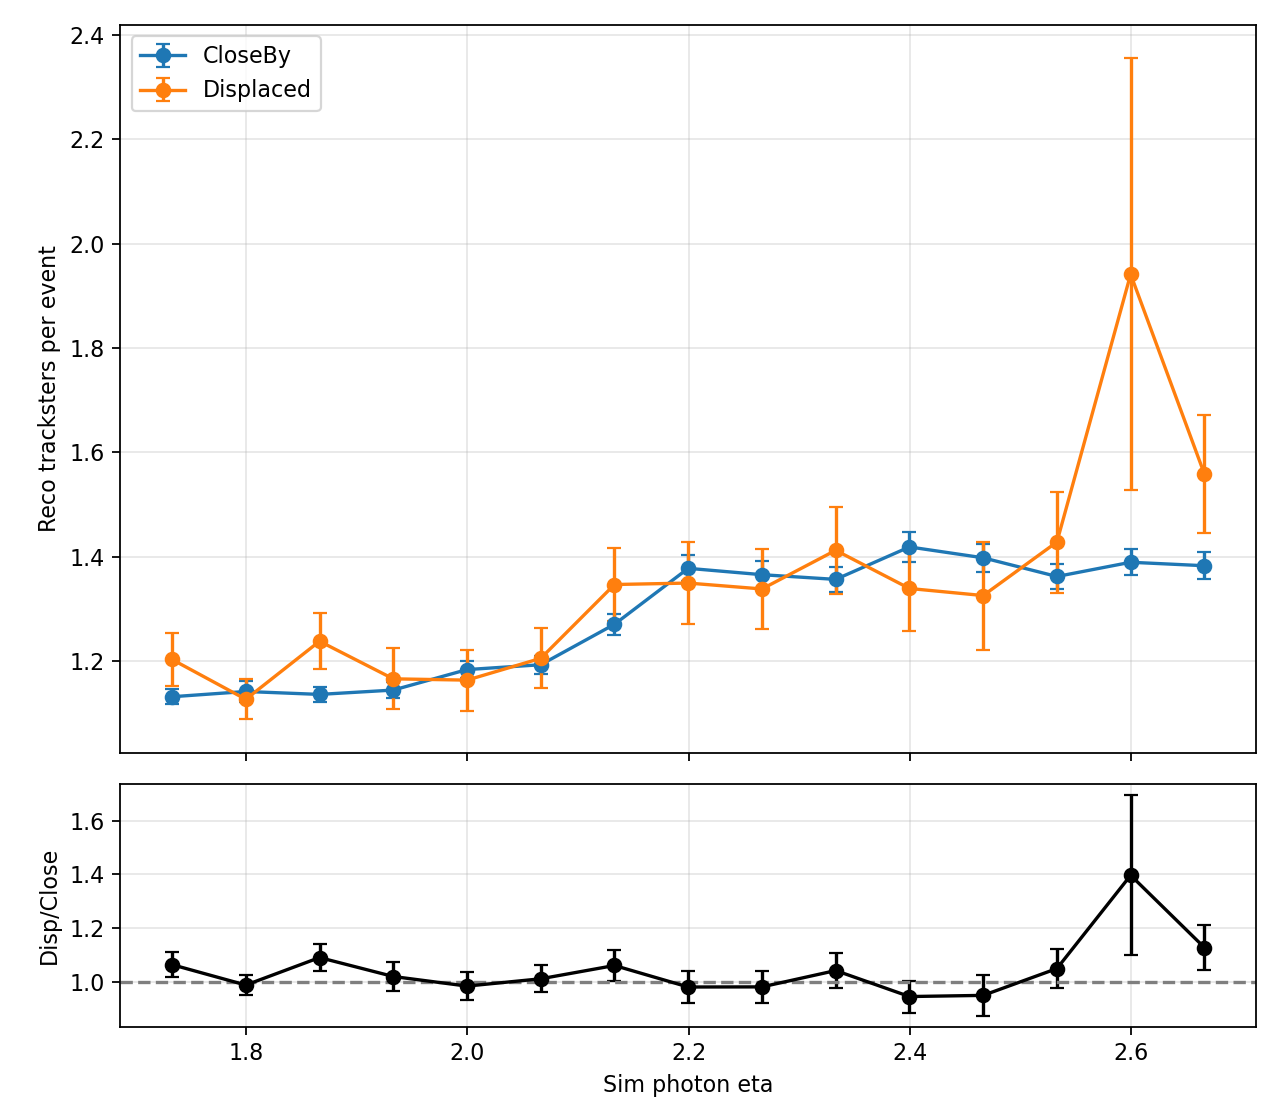
\includegraphics[width=\linewidth]{figures/gun_comparison_energy.png}
    \caption{Displaced gun sampling energy}
  \end{subfigure}
  \caption{Pointing-control comparison of the CloseBy and displaced guns. The upper panels show the mean number of
  reconstructed Tracksters per event versus simulated-photon pseudorapidity;
  each event contains one generated photon, so ideal reconstruction would give
  a multiplicity of one. Values above one indicate shower fragmentation.
  The lower panels show the displaced-to-CloseBy ratio. These plots
  compare the energy-sampling choices, rather than the timing correction.}
  \label{fig:guncomparison}
\end{figure*}

\subsection{Timing and validation of the pointing control}

Before interpreting displaced-shower failures, we tested the pointing limit
$\R=0$ against the existing CloseBy gun. Each event contains a single generated
photon, so ideally its shower would be reconstructed as exactly one Trackster;
a larger multiplicity signals fragmentation of that shower. At $\R=0$ the
displaced gun generates pointing trajectories and should reproduce the CloseBy
response when the kinematics and generation conditions are matched. Instead,
it initially produced substantially more Tracksters per event than CloseBy,
revealing excessive fragmentation even before any displacement was introduced.
Investigating this discrepancy exposed problems in the sample setup.

The first was the production time. The original gun assigned $t=0$ to a photon
created immediately before HGCAL, ignoring the flight time required to reach
that point. Its signals therefore arrived earlier than a particle travelling
at the speed of light from the interaction point could have reached the
calorimeter. Such arrival times are incompatible with the timing assumptions
of the hit-reconstruction chain, which rejected affected signals. The resulting
reconstructed energy was both severely reduced and unevenly retained across
the shower. This disrupted the energy deposits available for clustering,
breaking a single photon shower into several reconstructed Tracksters and
inflating the multiplicity. It was therefore a consequence of the
incorrect generation time, rather than evidence of a displacement-induced
clustering failure at $\R=0$.
The corrected implementation assigns a time from the path length and particle
velocity. More precisely, its present convention is
\begin{equation}
  ct_{\mathrm{prod}}=|\mathbf{x}_0|
       +\frac{|\mathbf{x}_{\mathrm{prod}}-\mathbf{x}_0|}{\beta},
  \qquad \beta=\frac{|\mathbf{p}|}{E},
  \label{eq:guntime}
\end{equation}
where the expression for $\beta$ uses $c=1$. The first segment, from the nominal
interaction point to the sampled origin, is assumed to be traversed at the
speed of light; the second uses the generated particle's velocity. For photons,
$\beta=1$. This is a prescribed timing convention rather than a sampled LLP
lifetime. At $\R=0$ it reduces to the ordinary photon flight time to the
production plane, about $\SI{11}{ns}$ for these geometries. Correcting the time
partially removed the anomalous behaviour of the pointing control.

A second difference was the sampled momentum variable. The displaced gun used
$p_T$ sampling, whereas the CloseBy reference sampled energy. By
Eq.~\eqref{eq:gunenergy}, the former generated much higher energies at large
pseudorapidity, where the showers split into more Tracksters. Introducing direct
energy sampling removed most of the remaining multiplicity discrepancy
(Fig.~\ref{fig:guncomparison}). Agreement is close over most of the displayed
range, with some differences in the highest-$\eta$ bins; the comparison
does not establish exact equivalence of the two samples.

Finally, the displaced-particle workflow used the
\texttt{DBrealisticHLLHC} beamspot smearing, which moved the carefully placed
production vertices and affected the truth-particle selection near the HGCAL
boundary. The workflow was changed to the \texttt{CloseBy} beamspot prescription
appropriate to particles generated at the calorimeter. Together, the timing,
energy-sampling and beamspot corrections established a usable pointing
reference for the displacement scans that follow.

\section{Reconstruction performance metrics}
\label{sec:metrics}

We will study how shower energy is distributed among reconstructed objects and contamination when several showers overlap.
We use the HGCAL validation framework, which associates reconstructed
Tracksters to SimTracksters by shared LayerCluster energy and from that defines efficiency, duplicate, merge and fake rates.

The association compares the per-LayerCluster energies of a SimTrackster $S$ and
a reconstructed Trackster $T$. The shared energy $E_{\mathrm{shared}}(S,T)$ is
the energy common to both, and the recovered fraction
$f_{ST}=E_{\mathrm{shared}}(S,T)/E_S$ is the fraction of the true shower energy
$E_S$ in a single reconstructed object. Two directional scores,
$s_{S\to T}$ and $s_{T\to S}$ (weighting squared energies, lower being better),
separately penalize SimTrackster energy missing from $T$ and reconstructed energy
in $T$ missing in $S$.

\subsection{Efficiency, duplicate, merge and fake rates}

For efficiency, a reconstructed Trackster $T$ is matched to a SimTrackster $S$
if $T$ holds more than half of $S$'s energy, i.e. if $f_{ST}>0.5$. A
SimTrackster is counted as efficient if at least one reconstructed Trackster is
matched to it. This criterion does not check whether that $T$ contains energy
from several SimTracksters.
Binned in a truth observable $B$ (e.g. displacement R), we define efficiency as
\begin{equation}
  \epsilon(B)=\frac{N_S(B;\ \exists T:\ f_{ST}>0.5)}{N_S(B)}.
  \label{eq:efficiency}
\end{equation}
For the duplicate rate, $T$ is matched to $S$ if $s_{S\to T}<0.6$; the rate
counts SimTracksters that match more than one reconstructed Trackster. For the
merge rate, $S$ is matched to $T$ if $s_{T\to S}<0.6$; the rate is defined on
reconstructed Tracksters, binned by reconstructed R, and counts T that have
 more than one S matching. The formal definitions are
\begin{equation}
  D(B)=\frac{N_S(B;\ \#\{T:s_{S\to T}<0.6\}\geq2)}{N_S(B)},
  \label{eq:duplicaterate}
\end{equation}
\begin{equation}
  M(B)=\frac{N_T(B;\ \#\{S:s_{T\to S}<0.6\}\geq2)}{N_T(B)}.
  \label{eq:mergerate}
\end{equation}
A reconstructed Trackster is fake if no SimTrackster matches it with
$s_{T\to S}<0.6$; the fake rate is the fraction of reconstructed Tracksters
that are fake. This matters especially with pileup: an algorithm can recover
the signal photon while also producing many unmatched Tracksters.
Small fragments can fail
this cut, so a low duplicate or merge rate does not by itself exclude
fragmentation; it is a caveat revisited in the two-shower study.

\subsection{Validation changes}
Making the merge, duplicate and other score thresholds configurable, displacement and timing observables, and a later refactoring that added
two-dimensional metrics in $\R$ and a second
variable, went into CMSSW pull requests
\#51510~\cite{DoljaninPR51510} and
\#51565~\cite{DoljaninPR51565}.

\section{How \cluethreed{} works}
\label{sec:clue3d}

\cluethreed{} is the existing CMS algorithm that groups LayerClusters across
calorimeter layers into Tracksters using the density-based idea of
CLUE~\cite{Rovere2020clue}. The studies use the default HLT \cluethreed{}
configuration without tuning for displaced showers, except where a parameter
variation is explicitly stated.

\subsection{Neighbourhoods projected from the interaction point}

Let LayerCluster $i$ have position $(x_i,y_i,z_i)$, transverse radius
$r_i=\sqrt{x_i^2+y_i^2}$, azimuth $\phi_i$, layer index $\ell_i$, and energy
$E_i$.
To compare a candidate $j$ with $i$, it projects $j$ onto the plane of $i$
along the ray from the origin through $j$. The projected radius is
\begin{equation}
  r_{j\to i}=z_i\frac{r_j}{z_j}.
\end{equation}
The squared transverse distance used by the implementation is then
\begin{equation}
  d_{XY}^2(i,j)=(r_i-r_{j\to i})^2
                    +r_{j\to i}^{\,2}(\Delta\phi_{ij})^2,
  \label{eq:clueprojective}
\end{equation}
where $\Delta\phi_{ij}$ is the azimuthal difference wrapped into
$[-\pi,\pi]$. The second term uses the small-angle arc distance in azimuth.
This is a projected distance, not Euclidean distance of the two LayerClusters. Exchanging $i$ and
$j$ changes the reference plane and can change its value, so $d_{XY}(i,j) \neq d_{XY}(j,i)$.

Candidate searches are restricted to three layers
before and after the reference layer. They also use nearby position-based
$(\eta,\phi)$ buckets called tiles: up to two tiles on either side for density estimation,
and one for the nearest-higher search.

\subsection{Density and Trackster formation}

The local density of LayerCluster $i$ is
\begin{equation}
  \rho_i=E_i+0.2\sum_{j\in\mathcal{N}_i}E_j,
  \label{eq:cluedensity}
\end{equation}
where $\mathcal{N}_i$ contains candidate LayerClusters on other layers with
$d_{XY}(i,j)<\dc$, and $\dc=\SI{1.8}{cm}$. The algorithm then finds the
nearest higher-density LayerCluster $h(i)$ from another layer, minimizing the
projected transverse distance, and records
$\delta_i=d_{XY}(i,h(i))$. This search can find neighbours beyond $\dc$;
if none is found, the distance is treated as infinite.

LayerClusters are classified as follows:
\begin{itemize}
  \item \textbf{Seeds} start new Tracksters. They require
  $\rho_i\geq\rhoc=\SI{0.6}{GeV}$ and separation from nearest higher:
  $\delta_i>\dm=\SI{1.8}{cm}$.
  \item \textbf{Outliers} have low density, $\rho_i<\rhoc$, and a distant
  nearest-higher neighbour, $\delta_i>2\dm=\SI{3.6}{cm}$.
  \item \textbf{Followers} are the remaining LayerClusters and inherit the
  Trackster assignment of their nearest-higher neighbour, if one exists.
\end{itemize}

Starting from each seed, its Trackster index is propagated through the
follower links (Fig.~\ref{fig:rechits-b}). Each assigned LayerCluster belongs
fully to one Trackster.
Outlier status propagates the same way: a follower whose nearest-higher chain
terminates in an outlier instead of seed is itself treated as an outlier.

\section{\cluethreed{} performance for displaced photons}
\label{sec:singlephoton}

The central question of this project is whether \cluethreed{} can reconstruct
a photon shower whose trajectory does not point back to the interaction
point. The displaced-photon study shows both a performance loss
and an unexpected structure: the loss develops in two stages, separated by a
plateau. The study shows that fragmentation induced by the origin-based
projection is the mechanism behind the observed loss.

\subsection{The performance loss is not a smooth decline}

We used single displaced photons without pileup, with Run4D121\footnote{The
CMSSW identifier for the specific Phase-2 detector geometry used in this
study.}
geometry and the default HLT \cluethreed{} configuration. The wide-range
production samples $\R$ uniformly from \SI{0}{cm} to \SI{350}{cm} and photon
energy from \SI{10}{GeV} to \SI{250}{GeV}, subject to the front and
back HGCAL-EE surface constraints described in Section~\ref{sec:gun}. We used 50\,000 events, each containing one displaced photon.

In addition to the efficiency of Section~\ref{sec:metrics}, I recorded the
largest fraction of each SimTrackster's energy captured by any one
reconstructed Trackster,
\begin{equation}
  f_{\max}(S)=\max_T\frac{E_{\mathrm{shared}}(S,T)}{E_S}.
  \label{eq:fmax}
\end{equation}
Efficiency is the fraction of SimTracksters with $f_{\max}>0.5$. Mean
$\langle f_{\max}\rangle$ measures energy recovery continuously, without
reducing each shower to a pass or fail, and does not have a threshold.

\begin{figure*}[!tp]
  \centering
  \begin{subfigure}[t]{0.54\textwidth}
    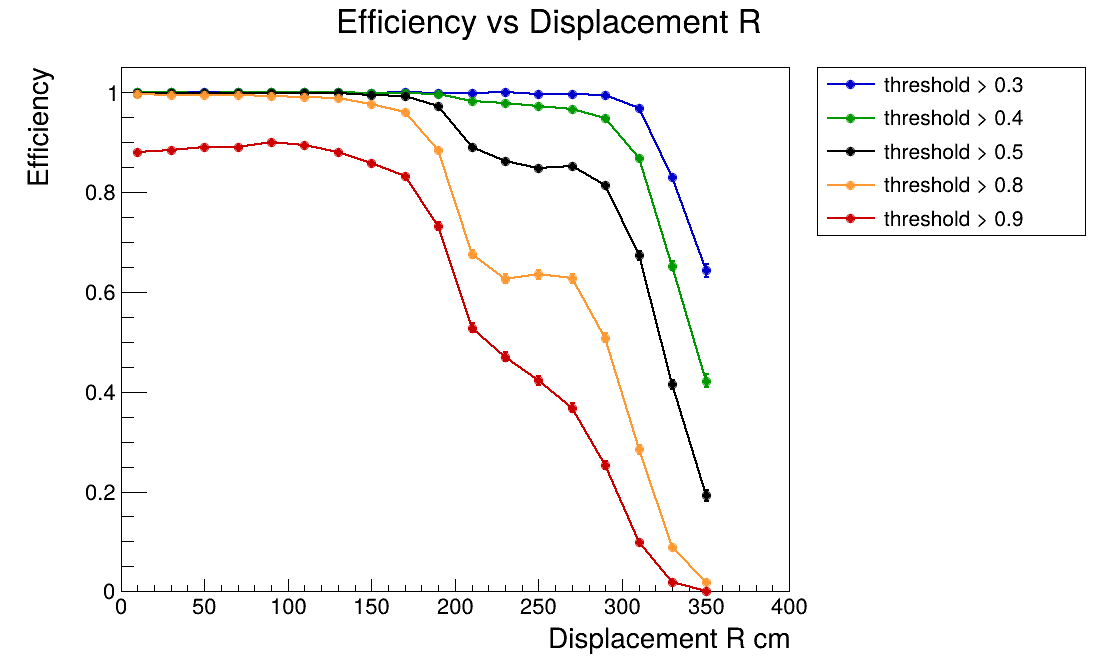
\includegraphics[width=\linewidth]{figures/singlephoton_efficiency_thresholds.png}
    \caption{Efficiency for several shared-energy requirements}
  \end{subfigure}\hfill
  \begin{subfigure}[t]{0.44\textwidth}
    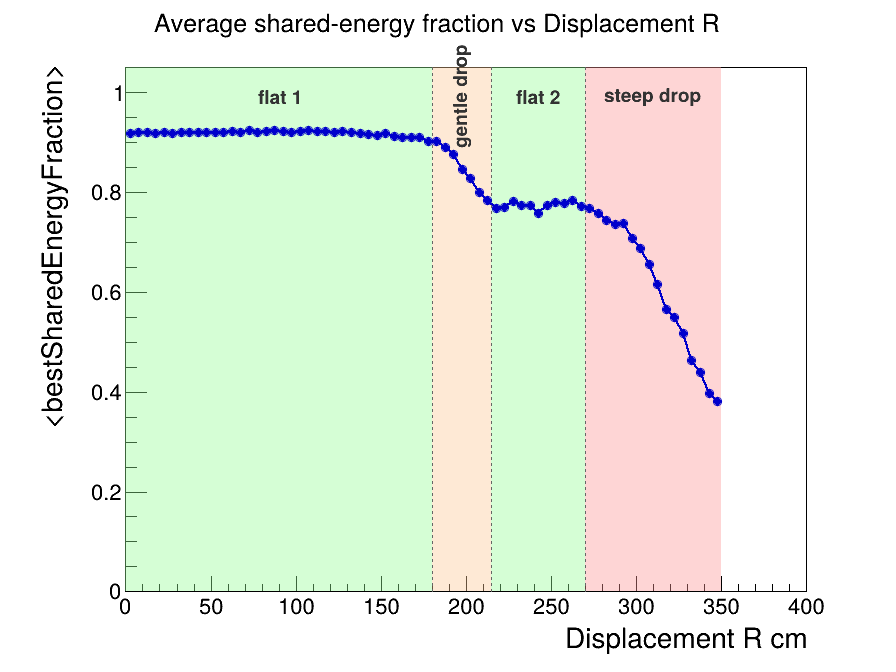
\includegraphics[width=\linewidth]{figures/singlephoton_mean_fraction.png}
    \caption{Mean largest shared-energy fraction}
  \end{subfigure}
  \caption{Single-photon reconstruction without pileup. (a) Efficiency for
  several shared-energy requirements; the black curve is the standard
  $f_{\max}>0.5$. (b) Mean $f_{\max}$, showing the two-stage loss and the
  intermediate plateau. Shaded regions are approximate slope regions.}
  \label{fig:singlephotonperformance}
\end{figure*}

Figure~\ref{fig:singlephotonperformance} shows that the loss is not a smooth
decline. The efficiency is high at small displacement and drops towards
the end, but in between there is a plateau, seen even more sharply in $\langle f_{\max}\rangle$.

This plateau is unexpected: increasing displacement should progressively
violate the pointing assumption, yet reconstruction temporarily stops
deteriorating. The feature persists whatever
shared-energy requirement is used, so it is not a consequence of the $0.5$
efficiency threshold. We will investigate real cause to efficiency loss and plateau.

\subsection{Testing geometric explanations}

\begin{figure}[!tp]
  \centering
  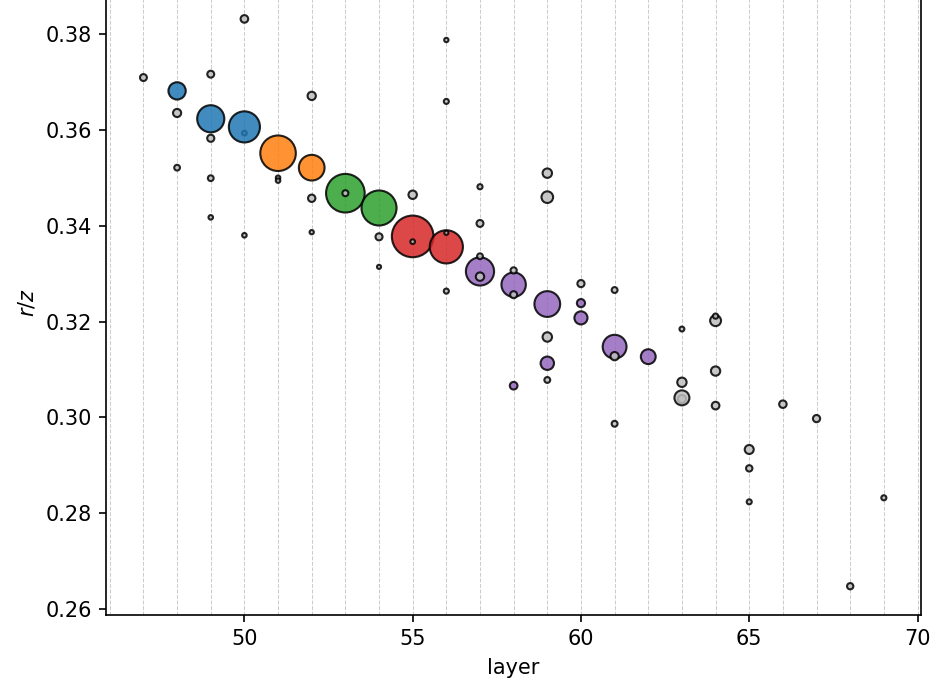
\includegraphics[width=\linewidth]{figures/singlephoton_split_R297_rz.png}
  \caption{A single photon at $\R\simeq\SI{297}{cm}$ split into five
  reconstructed Tracksters, shown as $r/z$ versus layer index. Colour identifies
  the reconstructed Trackster and marker size the energy; grey markers are
  outliers. The layer index follows the TICL convention, in which positive-endcap
  layers are offset to accommodate the negative endcap. $r/z$ is not constant.}
  \label{fig:singlephotonsplit}
\end{figure}

Some explanations can be ruled out quickly. The first is the limited
$(\eta,\phi)$ tile search: a displaced shower does not keep a constant
$(\eta,\phi)$ from layer to layer, so its LayerClusters could drift out of the
search window. But it was not the case, almost every LayerCluster
falls in the same tile as the shower core, at most one tile away, well within
the search reach, so no same-shower neighbour is lost to tiling. The
second explanation is a hidden dependence on trajectory orientation which causes plateau. However, separating photons by
$\Delta\phi(\phi_{\text{origin}}, \phi_{\text{surface}})$ left the plateau
intact, so the mixing of orientations under a
scalar $\R$ does not create the feature either.

\begin{figure}[!tp]
  \centering
  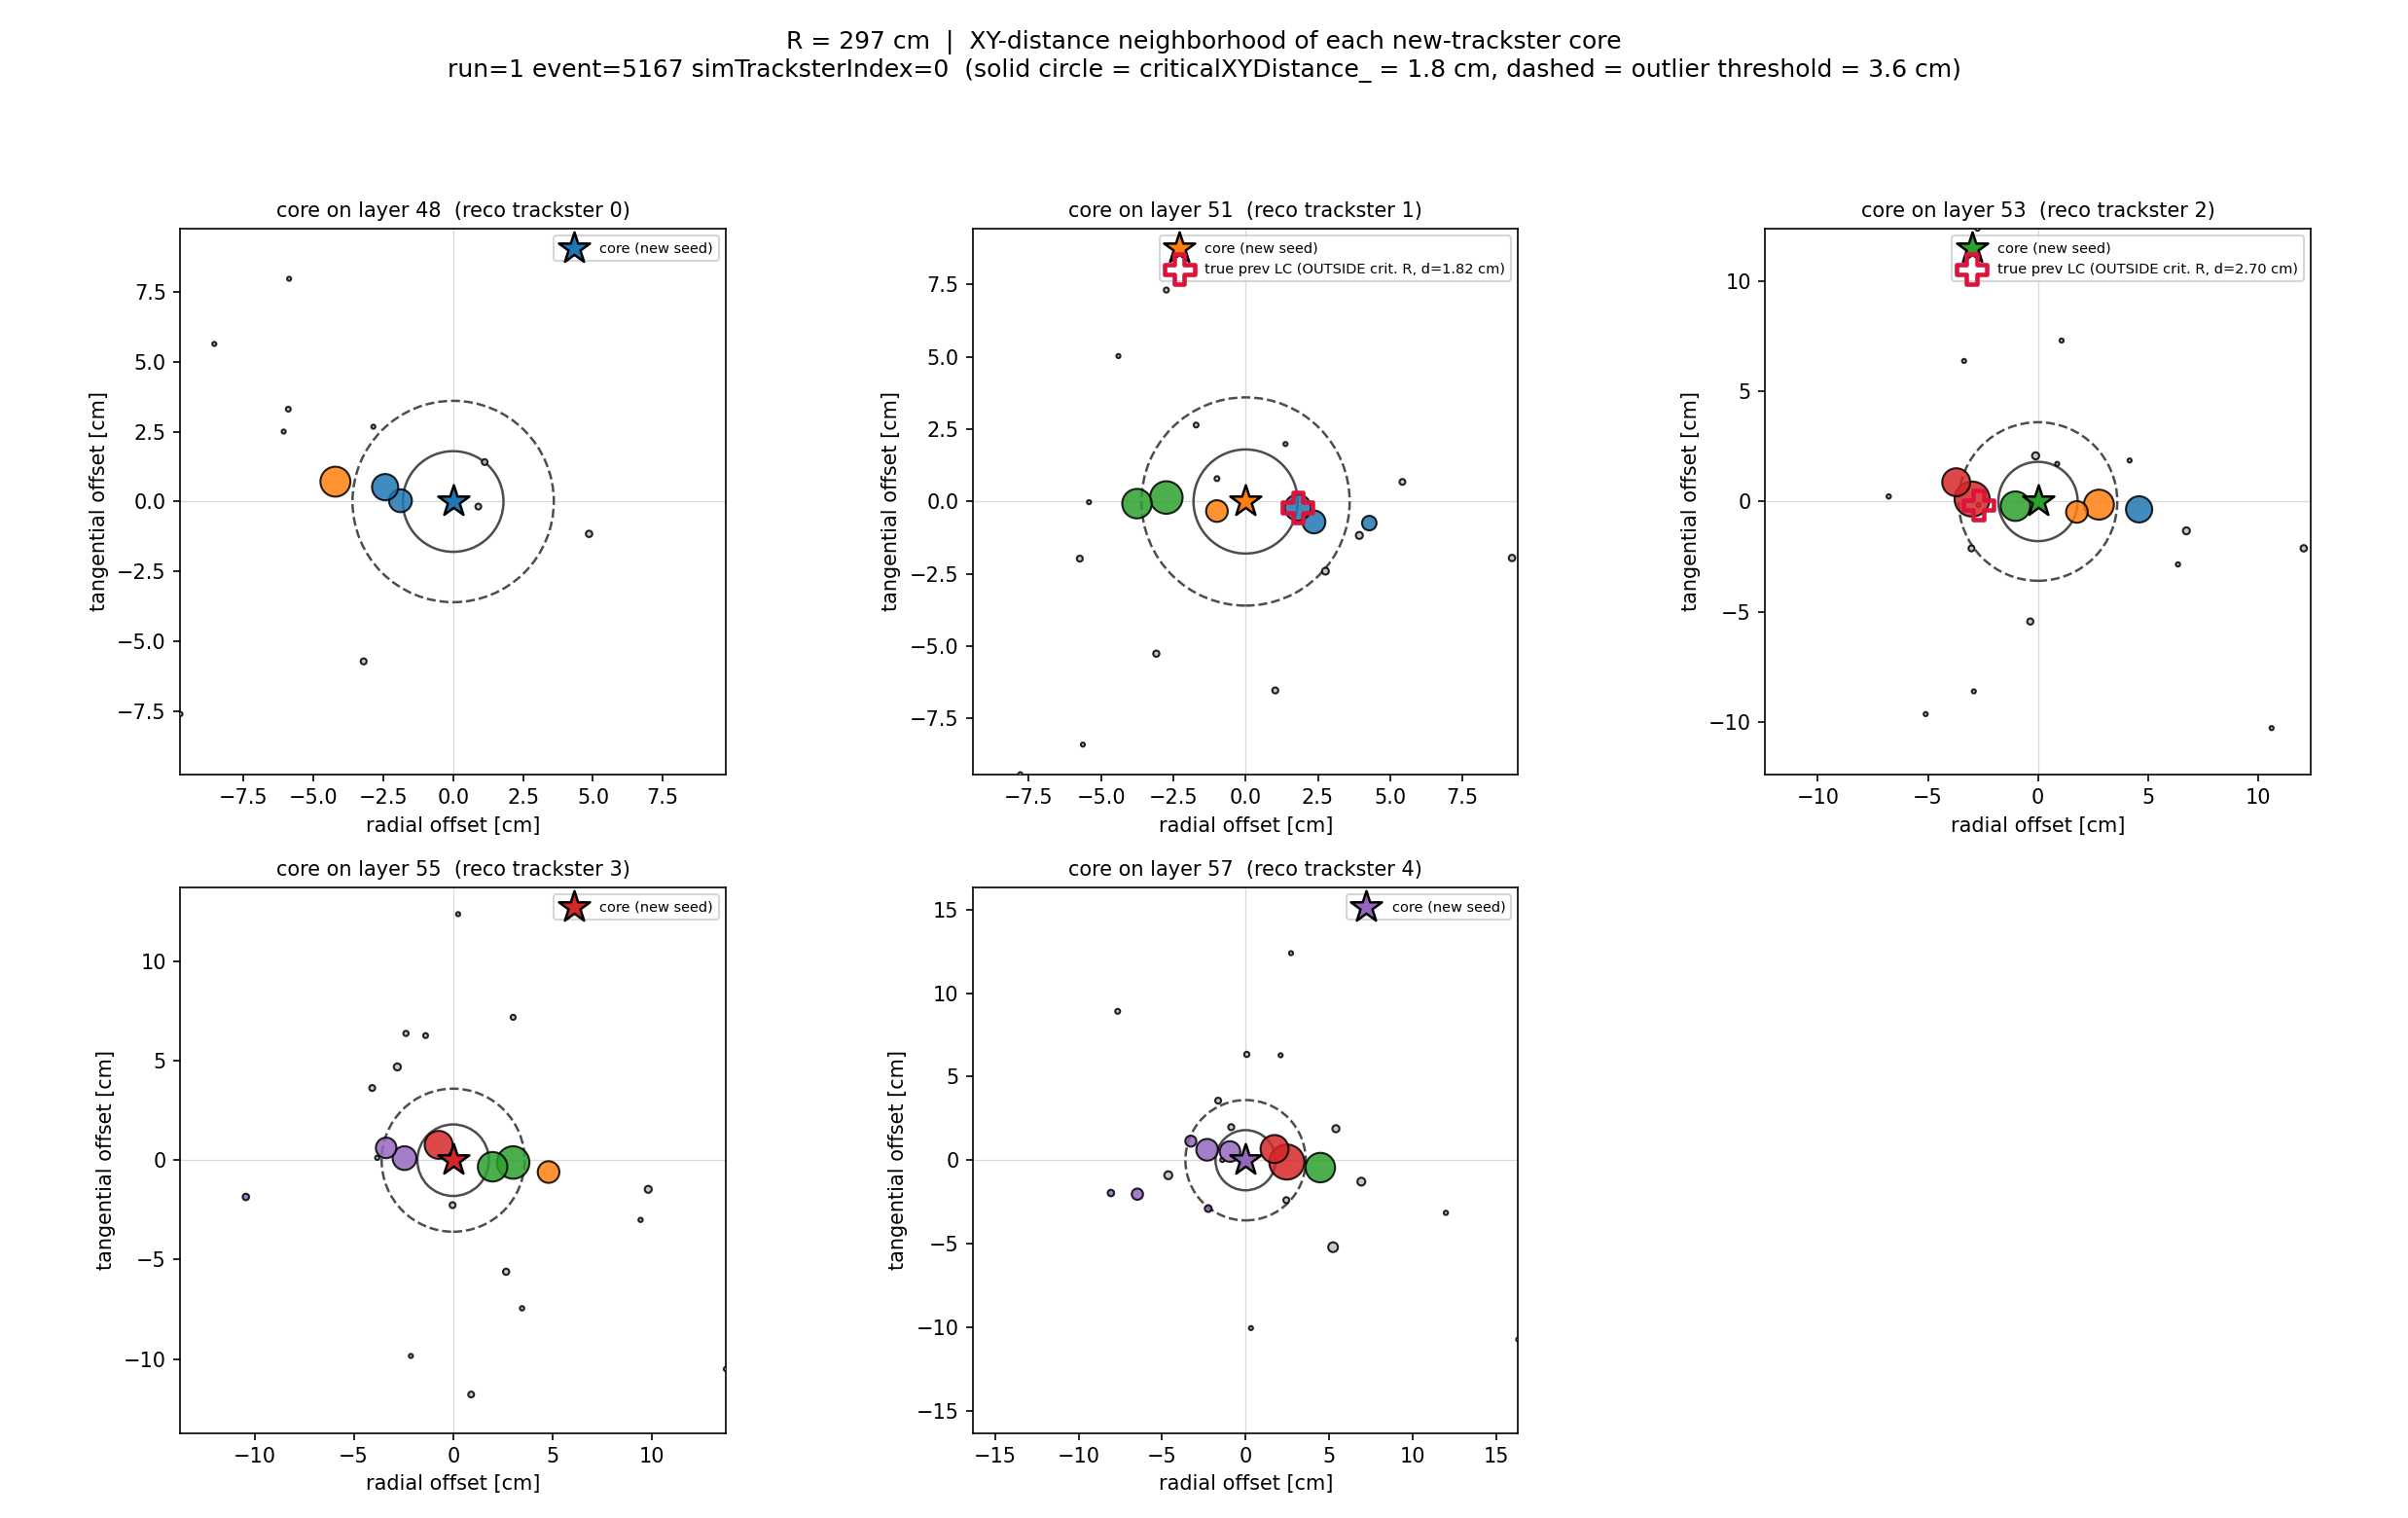
\includegraphics[width=\linewidth,trim=420bp 335bp 417bp 89bp,clip]{figures/singlephoton_neighbourhood_R297.png}
  \caption{A neighbourhood in the full projected coordinates for the
  $\R\simeq\SI{297}{cm}$ event previously shown in
  Fig.~\ref{fig:singlephotonsplit}. The star marks the layer-51 core of a new
  fragment, and circles the \SI{1.8}{cm} and \SI{3.6}{cm} distances.}
  \label{fig:singlephotonneighbourhood}
\end{figure}

\begin{figure*}[!tp]
  \centering
  \begin{subfigure}[t]{0.49\textwidth}
    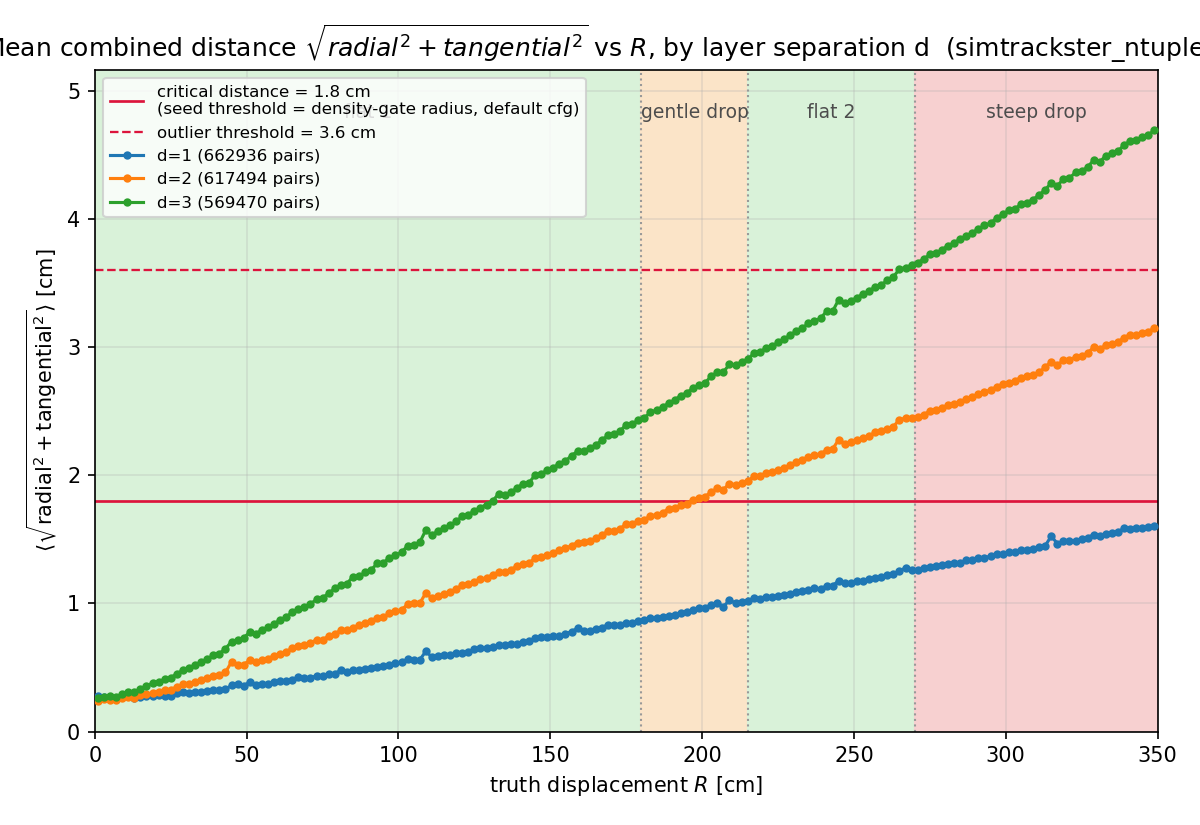
\includegraphics[width=\linewidth,trim=0 0 0 31bp,clip]{figures/singlephoton_pair_distance.png}
    \caption{Full projected distance for core-LC pairs}
    \label{fig:singlephoton-pair-distance}
  \end{subfigure}\hfill
  \begin{subfigure}[t]{0.49\textwidth}
    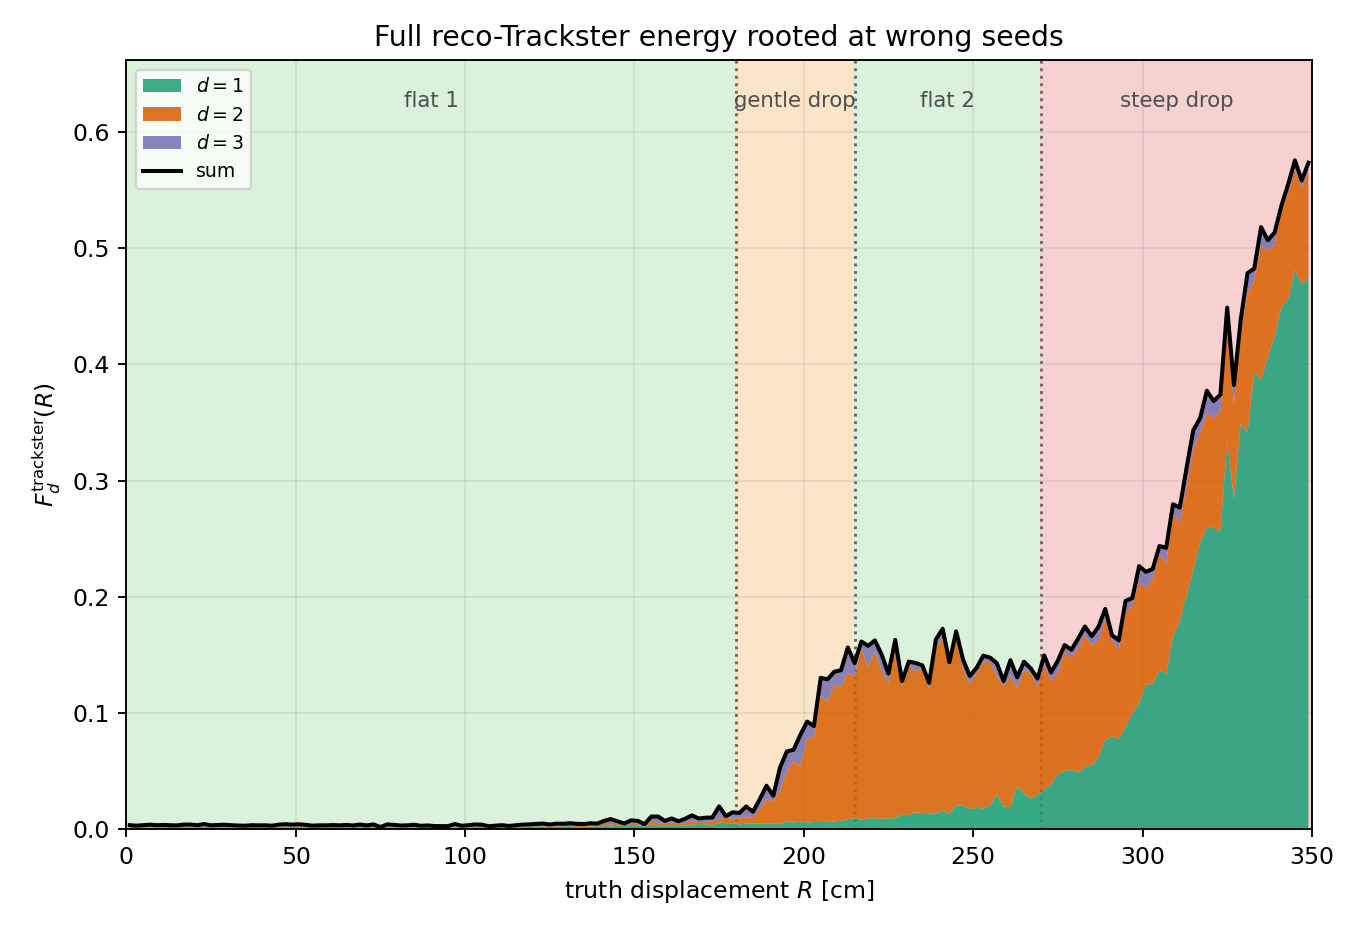
\includegraphics[width=\linewidth]{figures/singlephoton_seed_energy.png}
    \caption{Reconstructed energy in additional seeded fragments}
    \label{fig:singlephoton-seed-energy}
  \end{subfigure}
  \caption{The connection between the geometric threshold and fragmentation.
  (a) Mean full projected distance for LC pairs per $d$. (b) Full reconstructed energy in Tracksters whose
  seed has a higher-density candidate beyond $\SI{1.8}{cm}$, separated by the layer gap $d$ to
  that candidate.}
  \label{fig:singlephotongaps}
\end{figure*}

\subsection{The geometric origin of the growing distance}

The projected distance of Section~\ref{sec:clue3d} suggests a mechanism.
For a straight trajectory, transverse position is
\begin{equation}
  \mathbf{r}(z)=\mathbf{b}+z\mathbf{a},
  \qquad \R=|\mathbf{b}|,
  \label{eq:displacedline}
\end{equation}
where $\mathbf{a}$ is the transverse slope and $\mathbf{b}$ the position at
$z=0$. For a pointing trajectory $\mathbf{b}=0$: both $r/z$ and $\phi$ are
constant along the ideal shower axis. For a displaced trajectory,
$\mathbf{r}(z)/z=\mathbf{a}+\mathbf{b}/z$ changes with depth, as
Fig.~\ref{fig:singlephotonsplit} demonstrates for a real shower.

Projecting a point on layer $j$ to layer $i$ along a ray from the interaction
point gives
\begin{equation}
  \mathbf{r}_{j\to i}
    =\frac{z_i}{z_j}\mathbf{r}(z_j).
\end{equation}
Subtracting this projected position of $j$ from the position of $i$ gives:
\begin{align}
  \Delta\mathbf{r}_{ij}
    &=\mathbf{r}(z_i)-\mathbf{r}_{j\to i}\\
    &=\mathbf{b}\left(1-\frac{z_i}{z_j}\right)
     =\mathbf{b}\frac{z_j-z_i}{z_j}.
  \label{eq:projectionerror}
\end{align}
Thus the exact offset between ideal axis points is
$|\Delta\mathbf{r}_{ij}|=\R|z_j-z_i|/z_j$. For neighbouring layers, and
using the small-angle transverse metric implemented in \cluethreed{},
\begin{equation}
  \boxed{d_{XY}(i,j)\simeq\R\frac{|\Delta z|}{z}.}
  \label{eq:displacedscale}
\end{equation}

Equation~\eqref{eq:displacedscale} explains that distance grows with both
displacement and layer separation even for a perfectly straight photon.
It also gives the approximate scale at which a link exceeds the critical
distance,
\begin{equation}
  \R_{\mathrm{crit}}\simeq\frac{\dm z}{|\Delta z|}.
  \label{eq:criticaldisplacement}
\end{equation}
This supplies a prediction to test against the observed regions.

A first attempt looked promising but proved incomplete. Comparing, for the
most energetic LayerCluster on each layer, the offsets of pairs separated
by $d=1,2,3$ layers, the mean $d=3$ \emph{radial} ($r_i - r_{j \to i}$) offset reaches
$\SI{1.8}{cm}$ near the first decline and the $d=2$ offset near the
second, suggesting that links are lost as displacement
grows. This radial-only picture does not survive once the full projected
distance is used: the azimuthal term of $d_{XY}$ is not negligible, so the
crossings shift.



The local display in Fig.~\ref{fig:singlephotonneighbourhood} shows why the
full distance matters: the same-shower LC from another layer lies
$\SI{1.82}{cm}$ from another seed in projected coordinates, just
outside the critical circle, so two pieces of one continuous shower fall are not satisfying distance criterion.

\begin{figure*}[!tp]
  \centering
  \begin{subfigure}[t]{0.49\textwidth}
    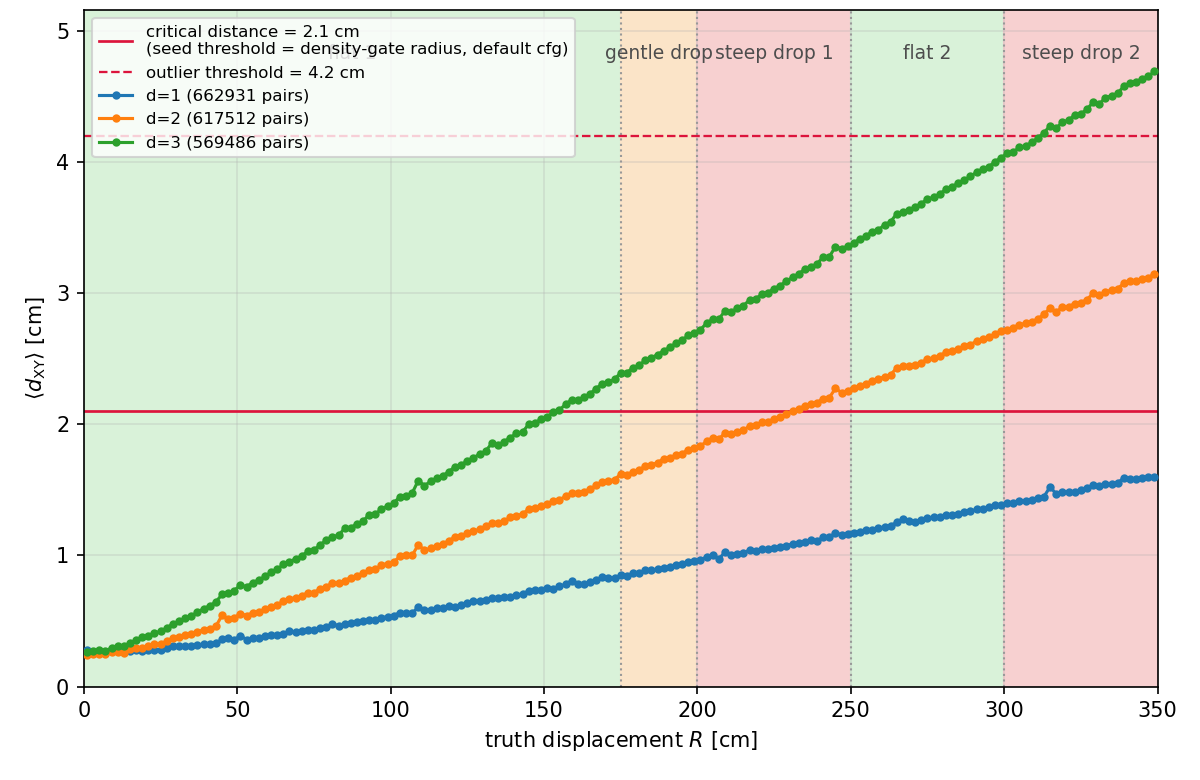
\includegraphics[width=\linewidth]{figures/singlephoton_ablation_pair_distance.png}
    \caption{Full projected distance for core-LC pairs}
  \end{subfigure}\hfill
  \begin{subfigure}[t]{0.49\textwidth}
    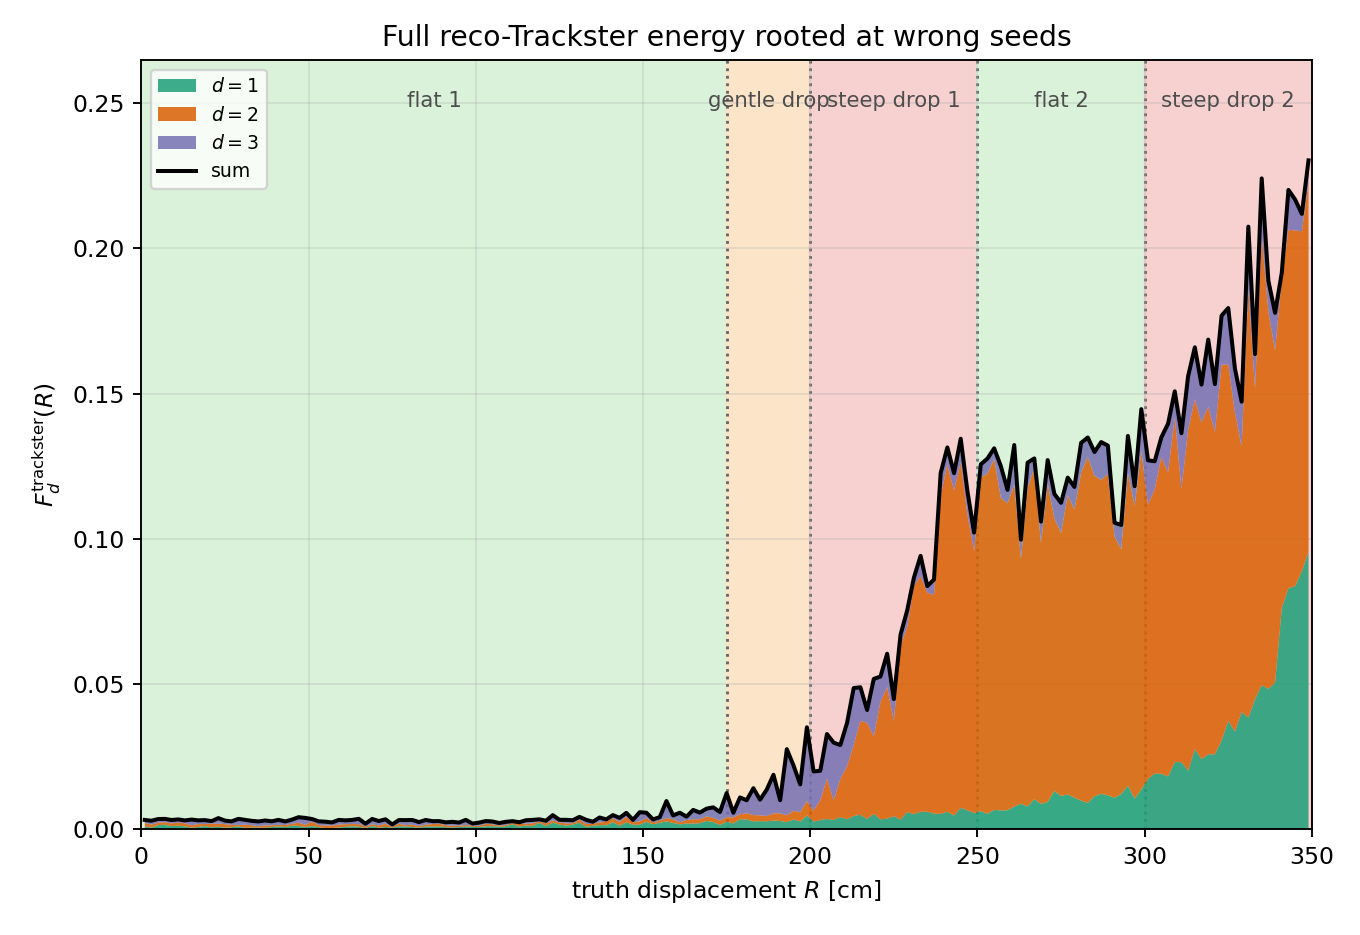
\includegraphics[width=\linewidth]{figures/singlephoton_ablation_seed_energy.png}
    \caption{Reconstructed energy in additional seeded fragments}
  \end{subfigure}
  \caption{The diagnostics of Fig.~\ref{fig:singlephotongaps} for
  $\dm=\SI{2.1}{cm}$.}
  \label{fig:singlephoton-ablation}
\end{figure*}

\subsection{The two-layer transition explains the first loss}



Important insight is shown in Fig.~\ref{fig:singlephoton-pair-distance}.
Near $\R\simeq\SI{200}{cm}$, the mean full projected distance for
$d=2$ pairs crosses $\SI{1.8}{cm}$. At the same time, as shown in
Fig.~\ref{fig:singlephoton-seed-energy}, the energy carried by reco
Tracksters which failed to follow nearestHigher $d=2$ layers away rises sharply. This connects the threshold to the objects that
actually remove energy from the best reconstructed match, which reduces efficiency.

The $d=2$ contribution rises from almost zero to roughly \SI{15}{\%} of the shower energy through the first decline. It then has plateau over
approximately the same displacement range as the plateau in
$\langle f_{\max}\rangle$. The plateau therefore corresponds to a region
where this newly important source of fragmentation has largely stabilized,
before the next one becomes dominant. At larger displacement, the green
$d=1$ contribution rises rapidly and drives the second, stronger loss of
captured energy.

Three-layer pairs cross $\SI{1.8}{cm}$ earliest, but remove little energy, because $d=1,2$ higher-density neighbour can still catch the LayerCluster and prevent a
split. And although the mean one-layer distance stays below $\SI{1.8}{cm}$ for every $R$, individual one-layer links still increasingly exceed it and produce the
observed contribution. This explains the first decline, the plateau and the
second decline.

\subsection{A controlled change of the critical distance}



As a direct test, I reran the HLT reconstruction on the same sample with the
seed distance raised from $\dm=\SI{1.8}{cm}$ to $\SI{2.1}{cm}$, with the density
radius fixed. By Eq.~\eqref{eq:criticaldisplacement} this should push each fragmentation stage to larger $\R$, and it does: the $d=2$ seeded
contribution turns on later, as shown in Fig.~\ref{fig:singlephoton-ablation}. The
degradation moves where the geometry predicts, suggesting
that it is caused by the projected-distance threshold and not just correlated
with displacement.


\section{Merging in two-photon events}
\label{sec:merging}

The single-photon study isolates fragmentation, but a useful reconstruction
must also keep neighbouring showers separate. Increasing the nearestHigher distance
can recover a displaced shower while allowing links to another particle.
I therefore extended the displaced-gun studies to two photons and examined both
the reconstructed objects and the nearest-higher-density links that form them.
All results in this section use the default \cluethreed{} configuration.

\subsection{Controlled shower separation}

Two complementary generators control the separation of the photons. In the
distance scan, the photons have equal energies and parallel momenta, while
their production points are shifted symmetrically by $\pm s/2$ in a randomly
chosen transverse direction. The sampled separations are
$s=1,2,4,8,16$~cm. Both trajectories must satisfy the gun's geometrical
acceptance. This gives a controlled comparison as the displacement is varied,
without changing the opening angle at the same time. The distance study uses
50\,000 generated events.

In the opening-angle scan, the two photons instead share a production point
and their momenta are rotated symmetrically around a central direction. The
angles are $\Delta\theta=0.001,0.004,0.016,0.064,0.256$~rad. Their physical
separation then grows along the shower depth. The two scans consequently test
different geometries: parallel, transversely separated showers and showers
that diverge from a common point.

\begin{figure*}[!tp]
  \centering
  \begin{subfigure}{0.88\textwidth}
    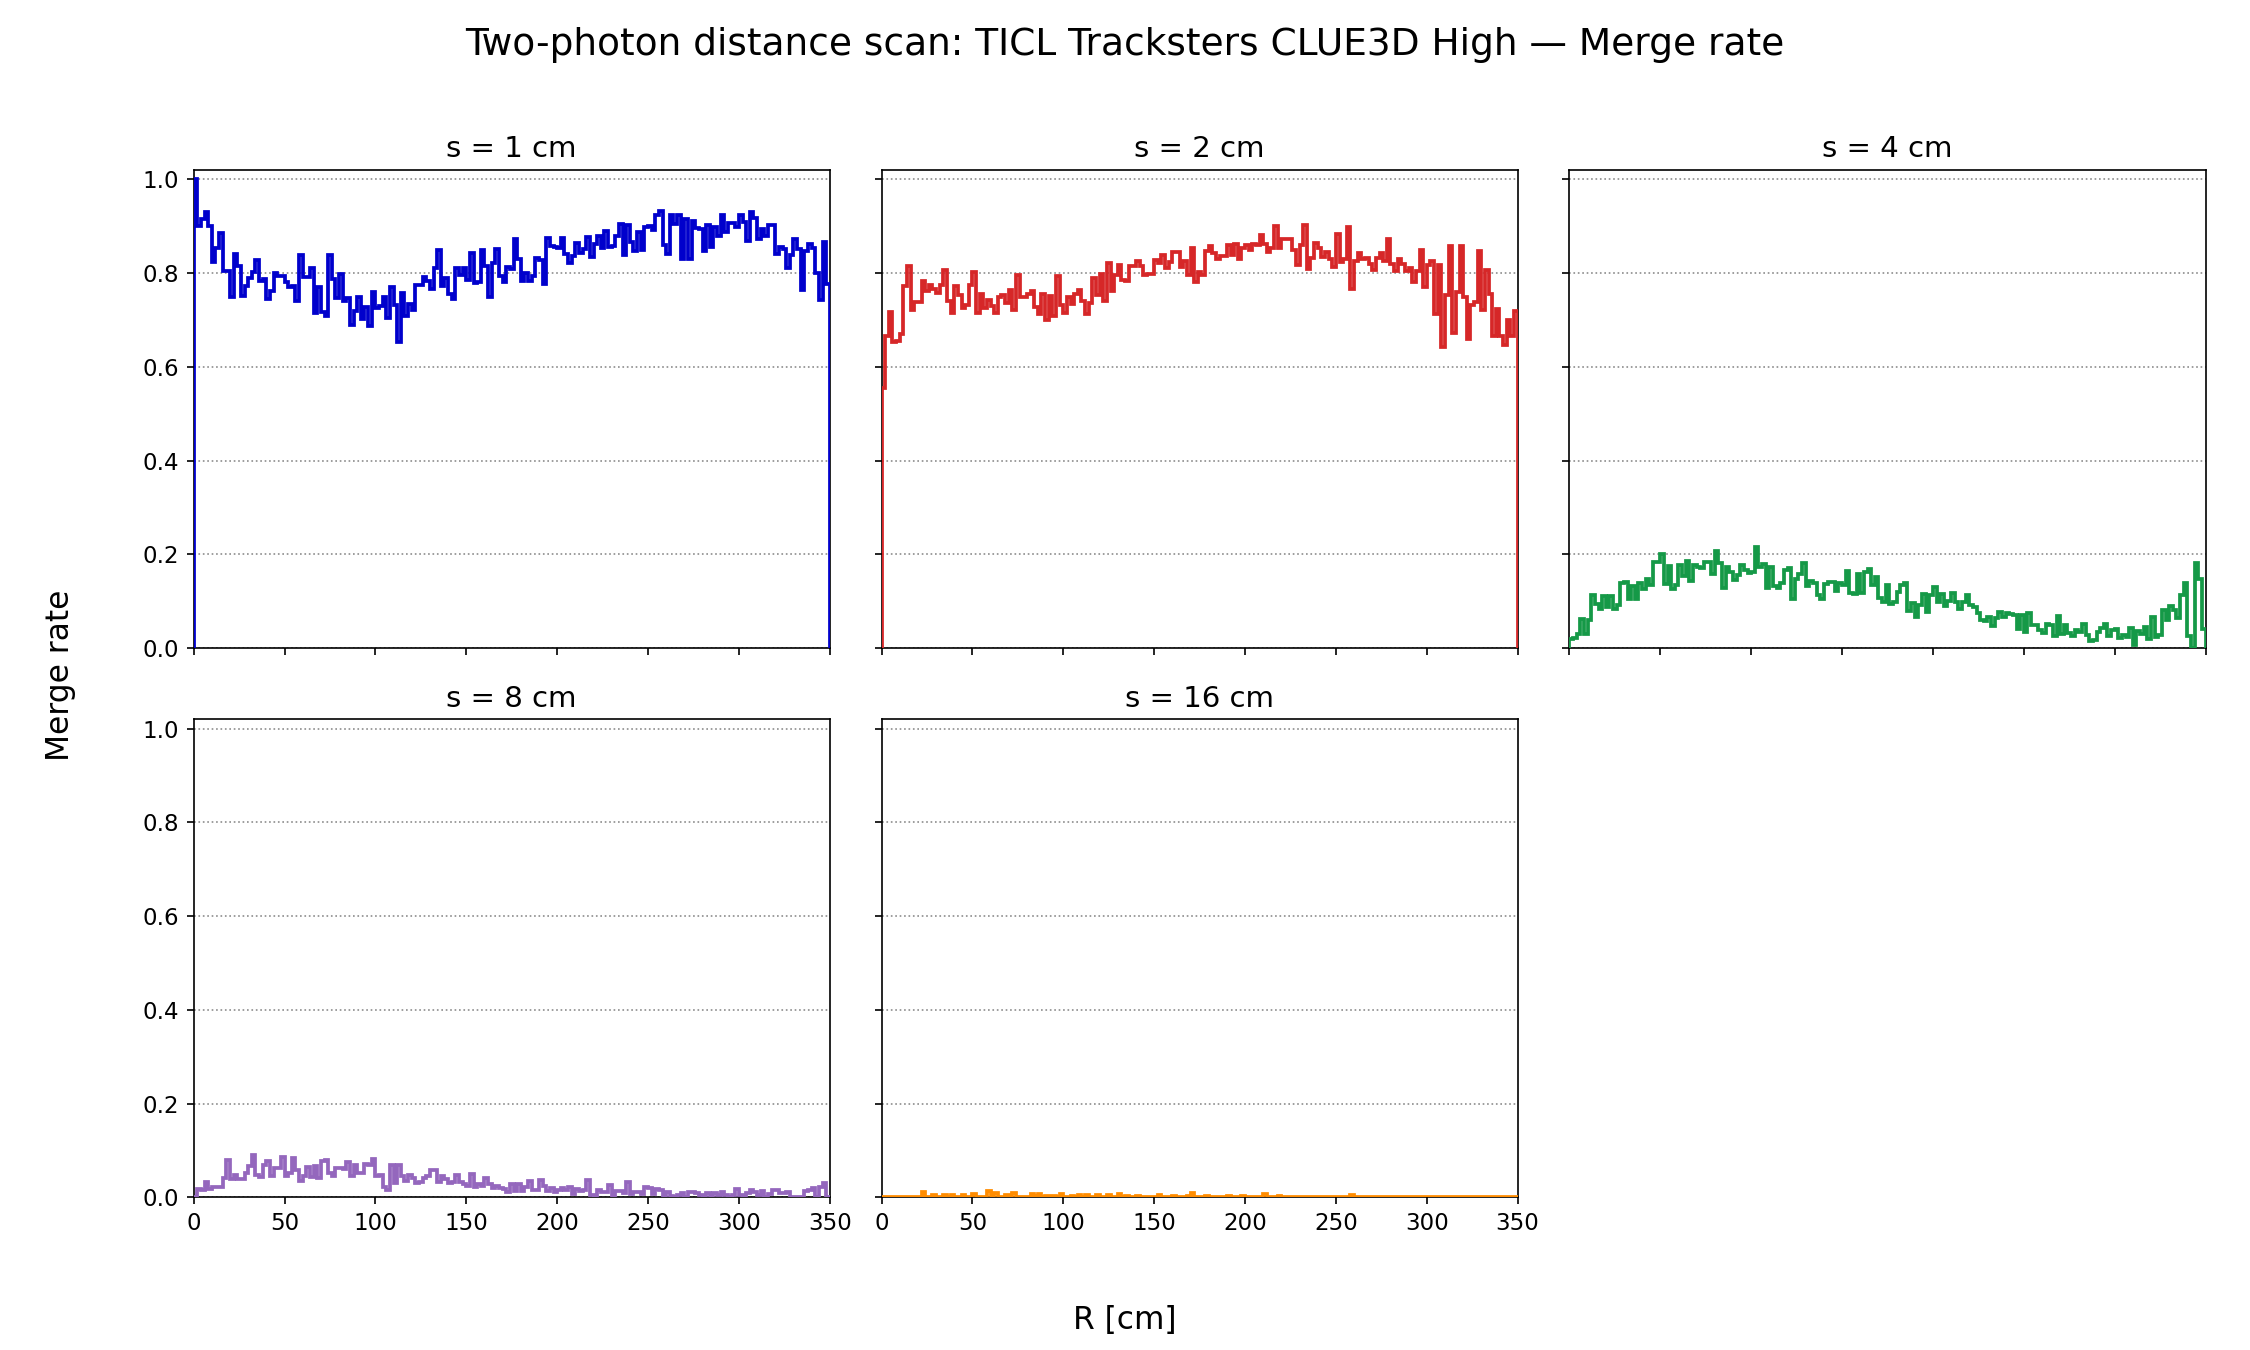
\includegraphics[width=\linewidth]{figures/merge_rate_distance.png}
    \caption{Reconstructed-object merge rate.}
    \label{fig:mergeratedistance}
  \end{subfigure}
  \par\medskip
  \begin{subfigure}{0.88\textwidth}
    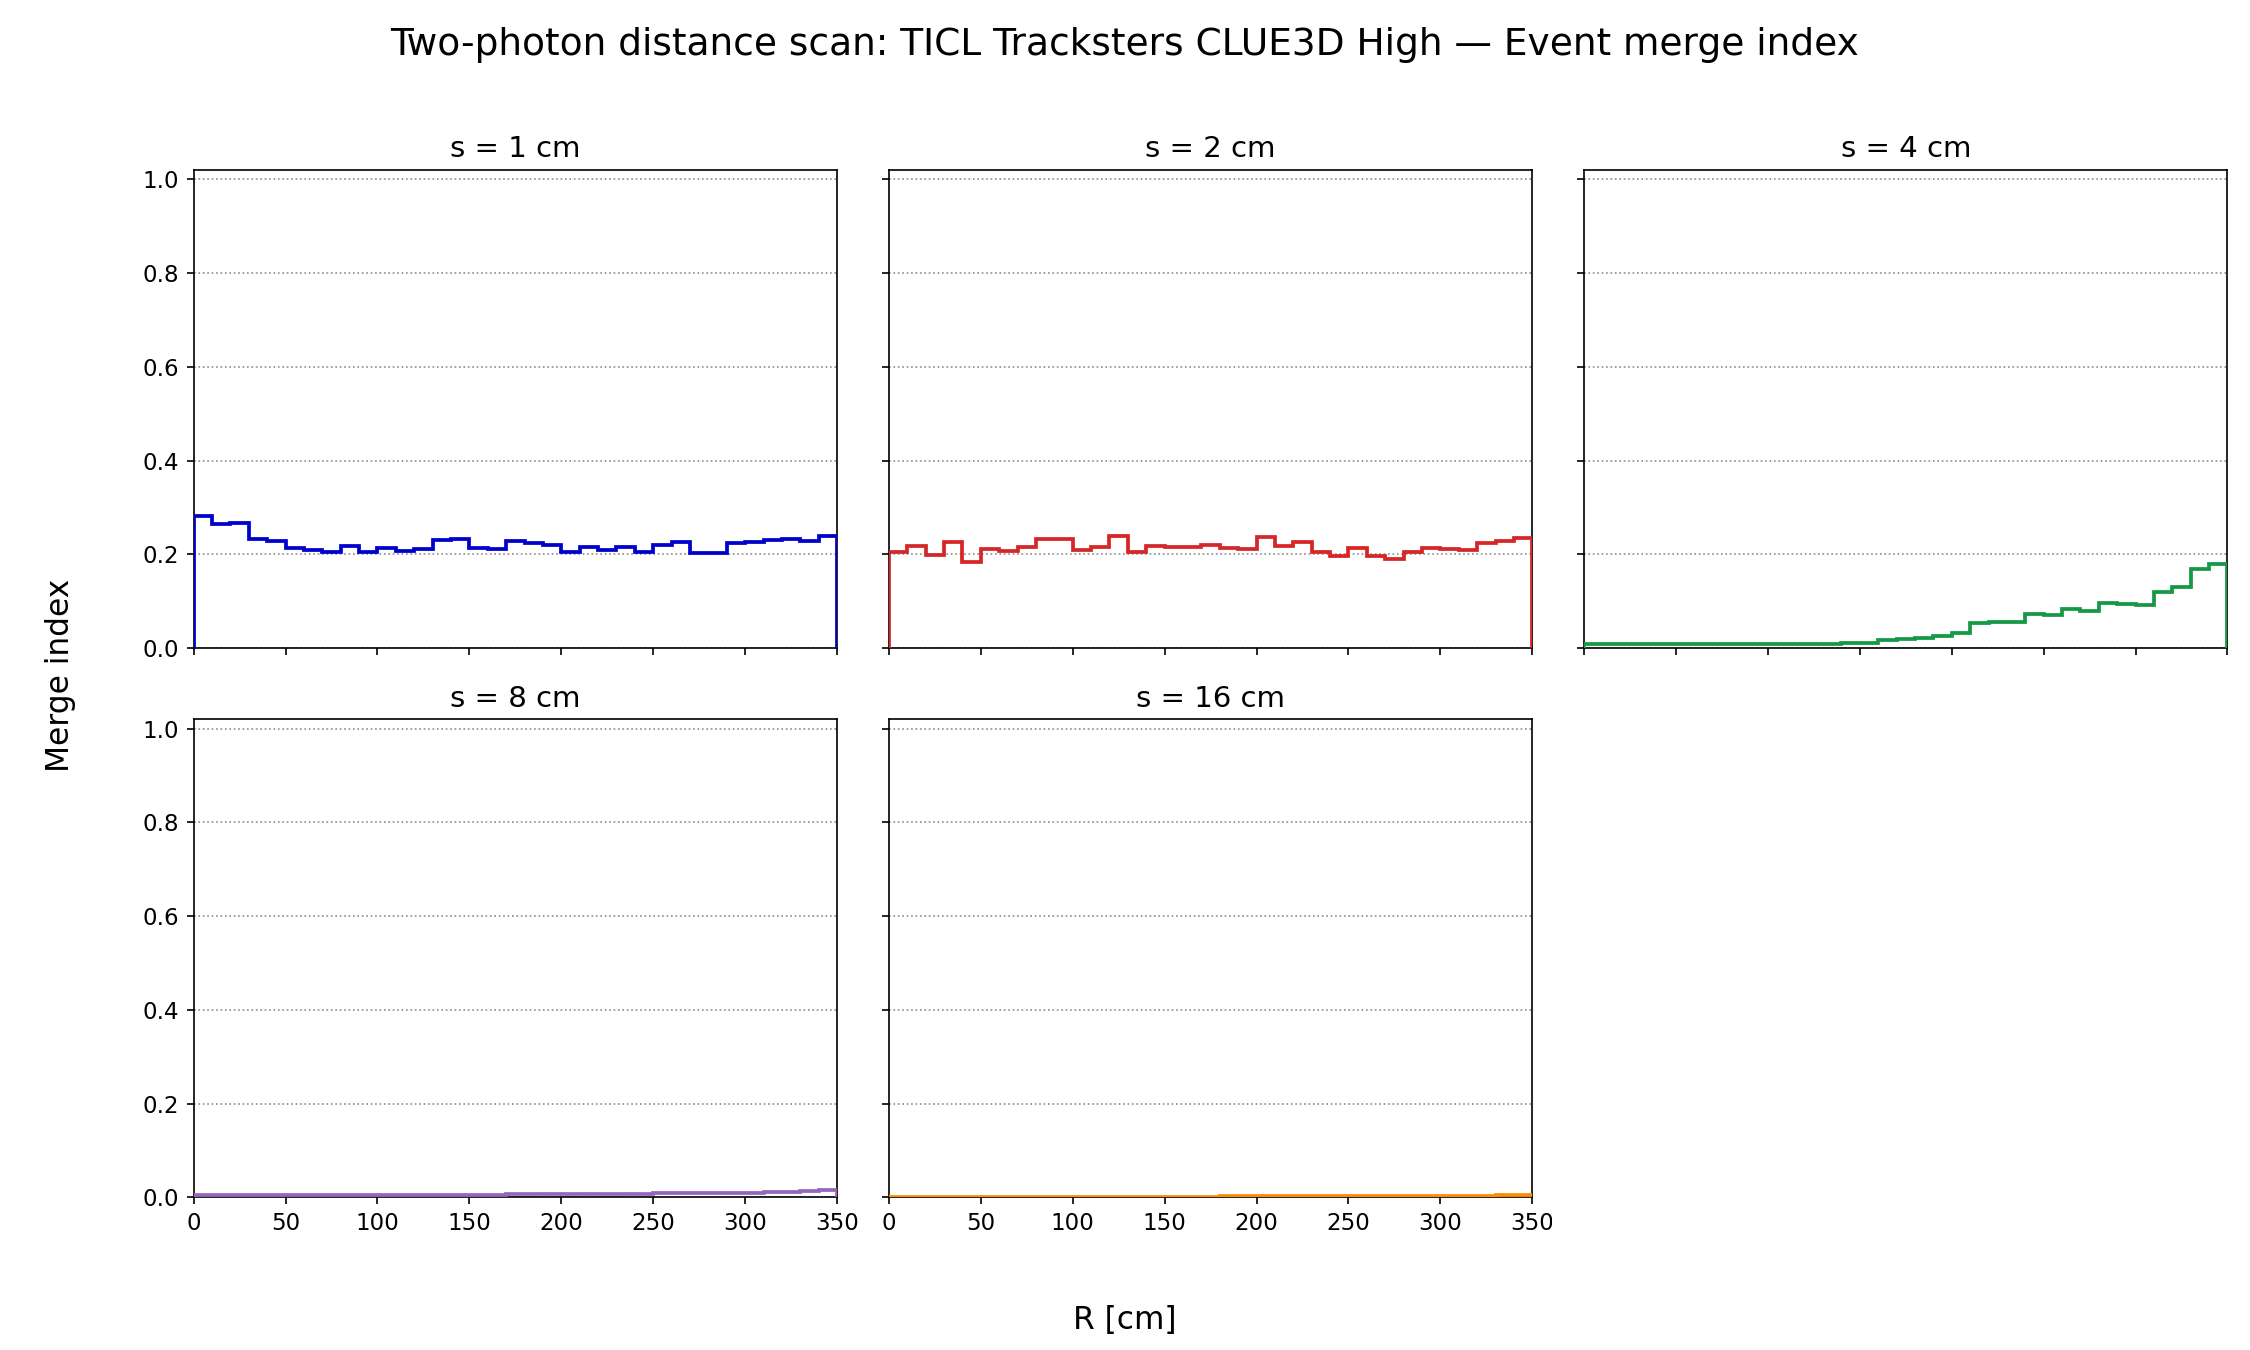
\includegraphics[width=\linewidth]{figures/merge_index_distance.png}
    \caption{Energy-weighted cross-shower link index.}
    \label{fig:mergeindexdistance}
  \end{subfigure}
  \caption{Two-photon distance scan with default \cluethreed{}. Each panel
  separates the five production-point distances. The object-based rate uses
  reconstructed $\R$, whereas the link index is binned using the truth
  displacement of the shower owning the follower LC. In particular, the
  $s=4$~cm index increases at large displacement even as the object-based merge
  rate falls.}
  \label{fig:mergingdistance}
\end{figure*}

For $s=4$~cm, the reconstructed-object merge rate initially appears
encouraging at large $\R$: after rising at intermediate displacement, it falls again
(Fig.~\ref{fig:mergeratedistance}). However, this is the same region in which
single showers fragment strongly. Splitting increases the number of
reconstructed objects in the denominator and can break an object that matched
two showers into smaller pieces that no longer pass both association cuts.
A decreasing merge rate therefore does not establish that the algorithm has
become better at separating the photons.

\subsection{A diagnostic based on the clustering links}

The object-based merge rate is distorted by fragmentation, so I introduced a
\emph{merge index} that measures cross-shower mixing directly from the
clustering links, without depending on how many Tracksters are produced. Every
follower LC $i$ records a nearest-higher neighbour $h(i)$; if $h(i)$ is owned by
a different truth shower than $i$, the algorithm has linked across the shower
boundary. The merge index is the energy-weighted fraction of follower energy in
such crossing links,
\begin{equation}
 I_{\mathrm{merge}}(B)=
 \frac{\sum_{i\in\mathcal{F}_B}E_i\,
 \mathbf{1}[o(h(i))\ne o(i),\ o(h(i))\text{ valid}]}
 {\sum_{i\in\mathcal{F}_B}E_i},
 \label{eq:mergeindex}
\end{equation}
where $o(\cdot)$ is the dominant truth-shower owner (the shower contributing the
largest truth energy fraction), $E_i$ the full LC energy, and $\mathcal{F}_B$
the truth-owned followers whose shower passes the truth selection in
displacement bin $B$ (seeds and outliers excluded). Energies are pooled across
the bin before the ratio is taken, so an index of $0.2$ means that $20\%$ of the
selected follower energy links into the wrong shower.

The index counts immediate links rather than the total energy ultimately
assigned to the wrong shower: one crossing link can redirect a whole chain of
followers, and seed and outlier decisions change which LCs enter the
denominator. These differences make it complementary to the object-based merge
rate.

Figure~\ref{fig:mergeindexdistance} resolves the apparent improvement. For
$s=4$~cm, the index rises from close to zero near the origin to about $0.18$
at large displacement. Cross-shower linking becomes more frequent even while
the reconstructed-object merge rate decreases. At $s=1$ and $2$~cm, substantial
mixing is already present, with an index of order $0.2$; the $8$ and $16$~cm
samples remain much cleaner. An index around $0.2$ should not be interpreted
as partial success at separating two almost overlapping showers: many links
can stay within their own dense core even when both cores ultimately feed the
same reconstructed object.

\subsection{Connection to the projective geometry}

\begin{figure*}[!tp]
  \centering
  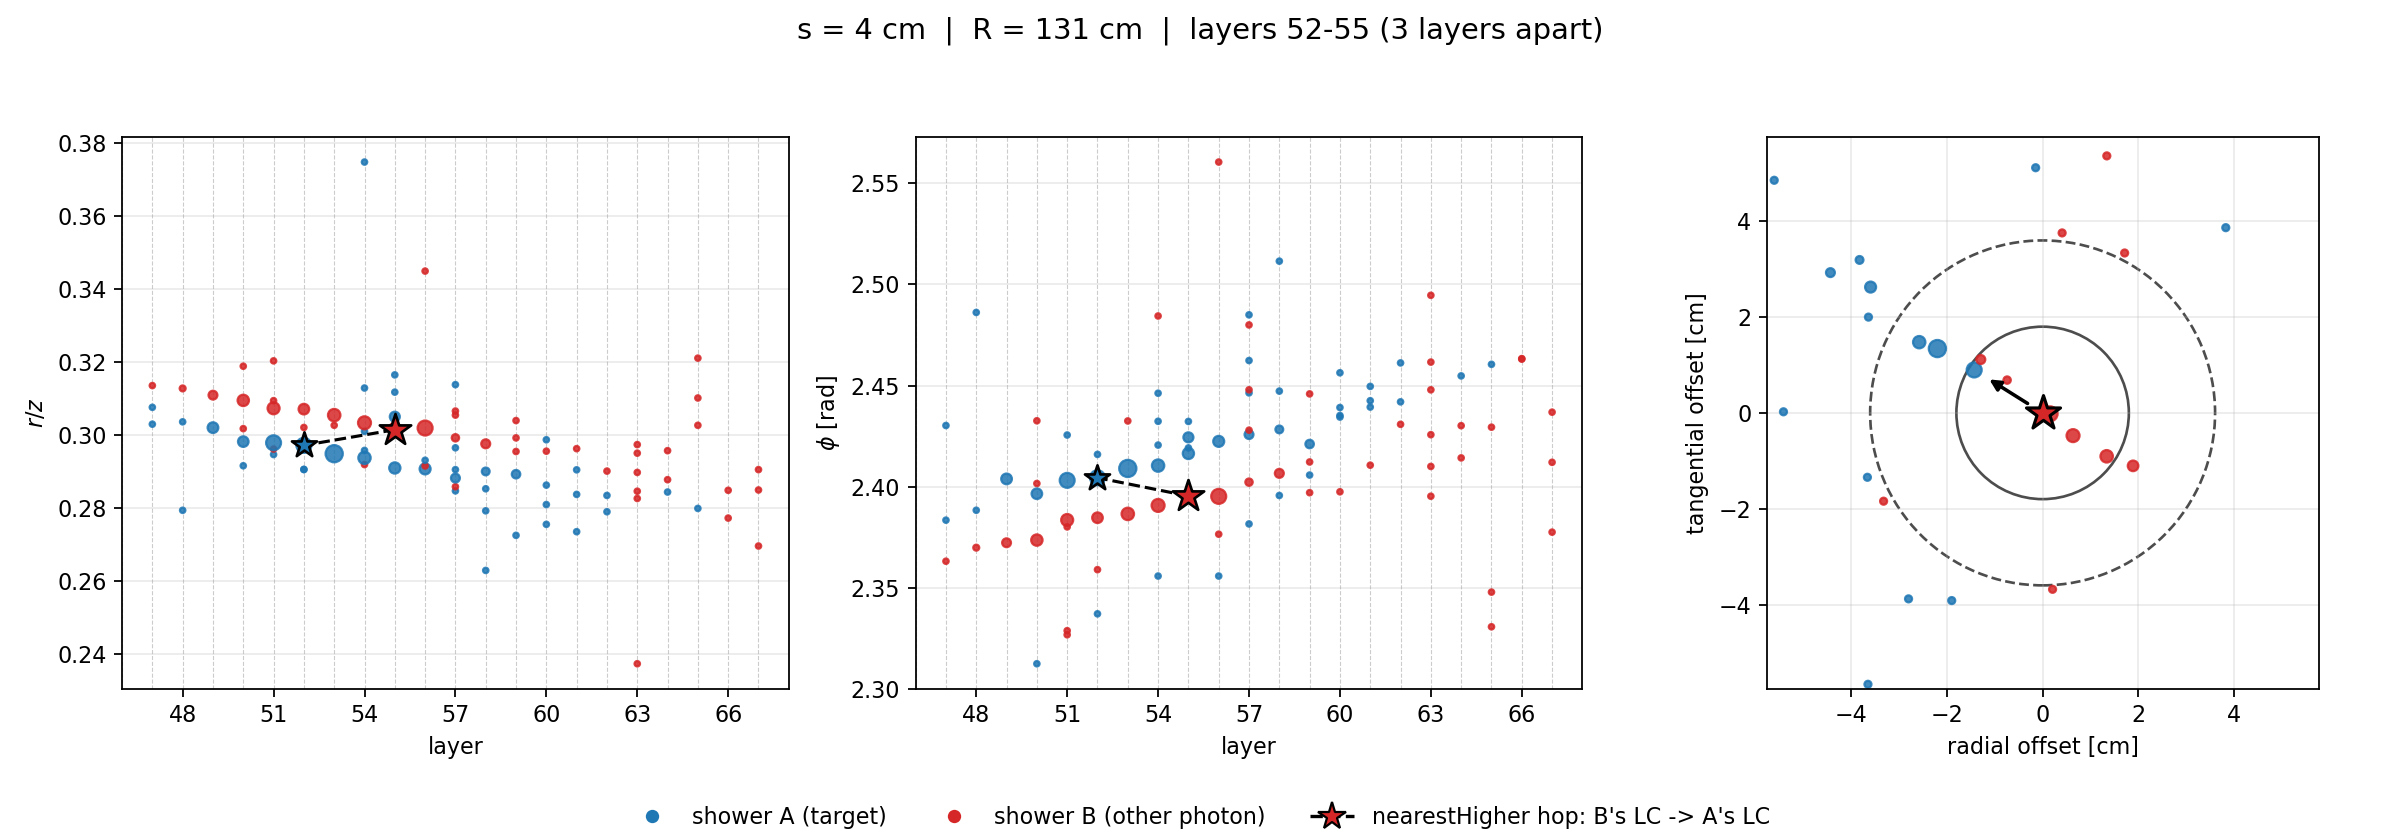
\includegraphics[width=\textwidth]{figures/merge_mechanism.png}
  \caption{An actual cross-shower nearest-higher link for photons separated
  by $s=4$~cm at $\R\simeq131$~cm. Blue and red identify the two truth
  showers. The highlighted LCs occupy layers 52 and 55, but have similar
  projective coordinates. The right panel shows neighbouring LCs projected
  onto the red LC's layer; the arrow follows its recorded link to shower
  $A$. The solid and dashed circles mark the 1.8~cm critical transverse
  distance and 3.6~cm outlier distance.}
  \label{fig:mergemechanism}
\end{figure*}

Figure~\ref{fig:mergemechanism} shows an individual cross-shower link, in an
event with $s=4$~cm and $\R\simeq131$~cm. The highlighted red LC belongs to
shower $B$, but its recorded nearest-higher neighbour is the blue LC from
shower $A$, three layers away. The first two panels show why this link is
geometrically possible: the two LCs have similar $r/|z|$ and $\phi$ despite
belonging to different showers, so that in the third panel the blue neighbour
lies inside the 1.8~cm circle once projected onto the red LC's layer. The
algorithm therefore sees a reachable higher-density neighbour across the truth
boundary, tying the cross-shower links to the observed merged objects.

The origin projection discussed in Section~\ref{sec:singlephoton} can also
explain how links cross between the showers. Consider ideal parallel axes
$\mathbf{x}_A(z)=\mathbf{b}_A+z\mathbf{a}$ and
$\mathbf{x}_B(z)=\mathbf{b}_A+\mathbf{s}+z\mathbf{a}$, where
$\mathbf{b}_A$ is shower $A$'s transverse intercept at $z=0$ and
$\mathbf{s}$ is their transverse separation, with $|\mathbf{s}|=s$. Projecting a point on shower
$B$ at $z_j$ onto the layer of a point on shower $A$ at $z_i$ gives distance:
\begin{equation}
 \mathbf{x}_A(z_i)-\frac{z_i}{z_j}\mathbf{x}_B(z_j)
 =\mathbf{b}_A\frac{z_j-z_i}{z_j}-\frac{z_i}{z_j}\mathbf{s}.
 \label{eq:crossshowerprojection}
\end{equation}
The first term is the displacement-induced offset derived for one shower;
the second represents the true separation of the pair. For suitable layer
ordering and separation direction, these terms partly cancel. Points from
different showers can then appear close in the projected plane even while
points along one shower are pushed apart.

\subsection{Which layer gaps produce the merging?}

\begin{figure*}[!tp]
  \centering
  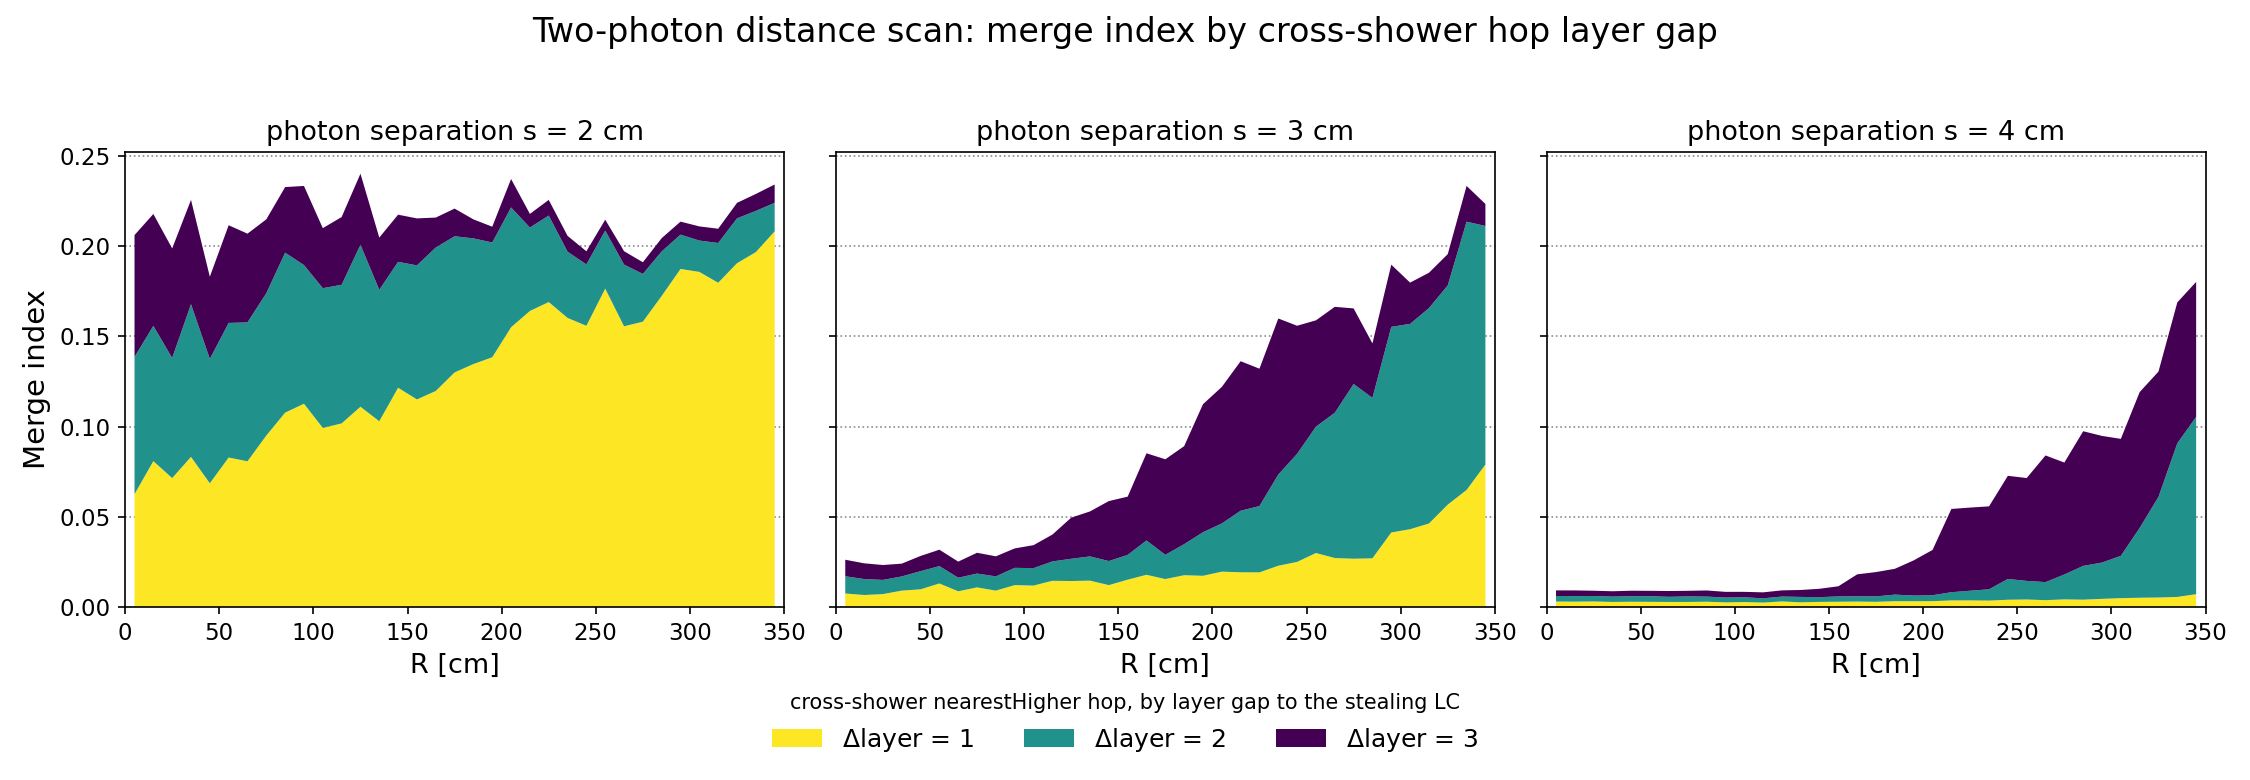
\includegraphics[width=\textwidth]{figures/merge_index_layergap.png}
  \caption{Merge index decomposed by the layer gap of cross-shower
  nearest-higher links for photon separations $s=2,3,4$~cm. Yellow, teal and
  purple correspond to one-, two- and three-layer gaps. All bands use the
  same follower-energy denominator, so their heights sum to the merge index.
  Larger separations favour larger gaps at the onset of mixing; increasing
  displacement makes smaller-gap contributions more important. The 3~cm
  panel comes from the finer separation scan.}
  \label{fig:mergegaps}
\end{figure*}

To see whether the three-layer link of Fig.~\ref{fig:mergemechanism} is
representative, I split the merge-index numerator by the layer gap
$\Delta\ell=|\ell_i-\ell_{h(i)}|$ between each follower and its cross-shower
neighbour, keeping the same denominator so the $\Delta\ell=1,2,3$ bands sum to
the merge index (Fig.~\ref{fig:mergegaps}, for $s=2,3,4$~cm).

The dominant gap shifts with separation. At $s=2$~cm, adjacent-layer links
carry most of the cross-shower energy and grow with $\R$. At $s=3$~cm the onset
is led by three-layer links, overtaken by two-layer links at larger $\R$. At
$s=4$~cm three-layer links dominate the onset and most of the growth, with
two-layer links rising only near the end of the scan. The event display of
Fig.~\ref{fig:mergemechanism} therefore shows the link type that drives the
onset for the $4$~cm pair, not an isolated coincidence.

This ordering follows from how the projection offset scales. Bridging the
separation $s$ requires offset, and since the offset grows with the
layer gap $\Delta z$, a wider gap reaches that offset at smaller $\R$. Wide-gap
links therefore start crossing first; as $\R$ increases, progressively
shorter-gap links reach the same offset and begin merging too. This is the
shift towards smaller gaps with displacement seen in the stacked bands, and it
explains not just that the merge index rises but which links carry the rise.

\subsection{Opening-angle scan}

\begin{figure*}[!tp]
  \centering
  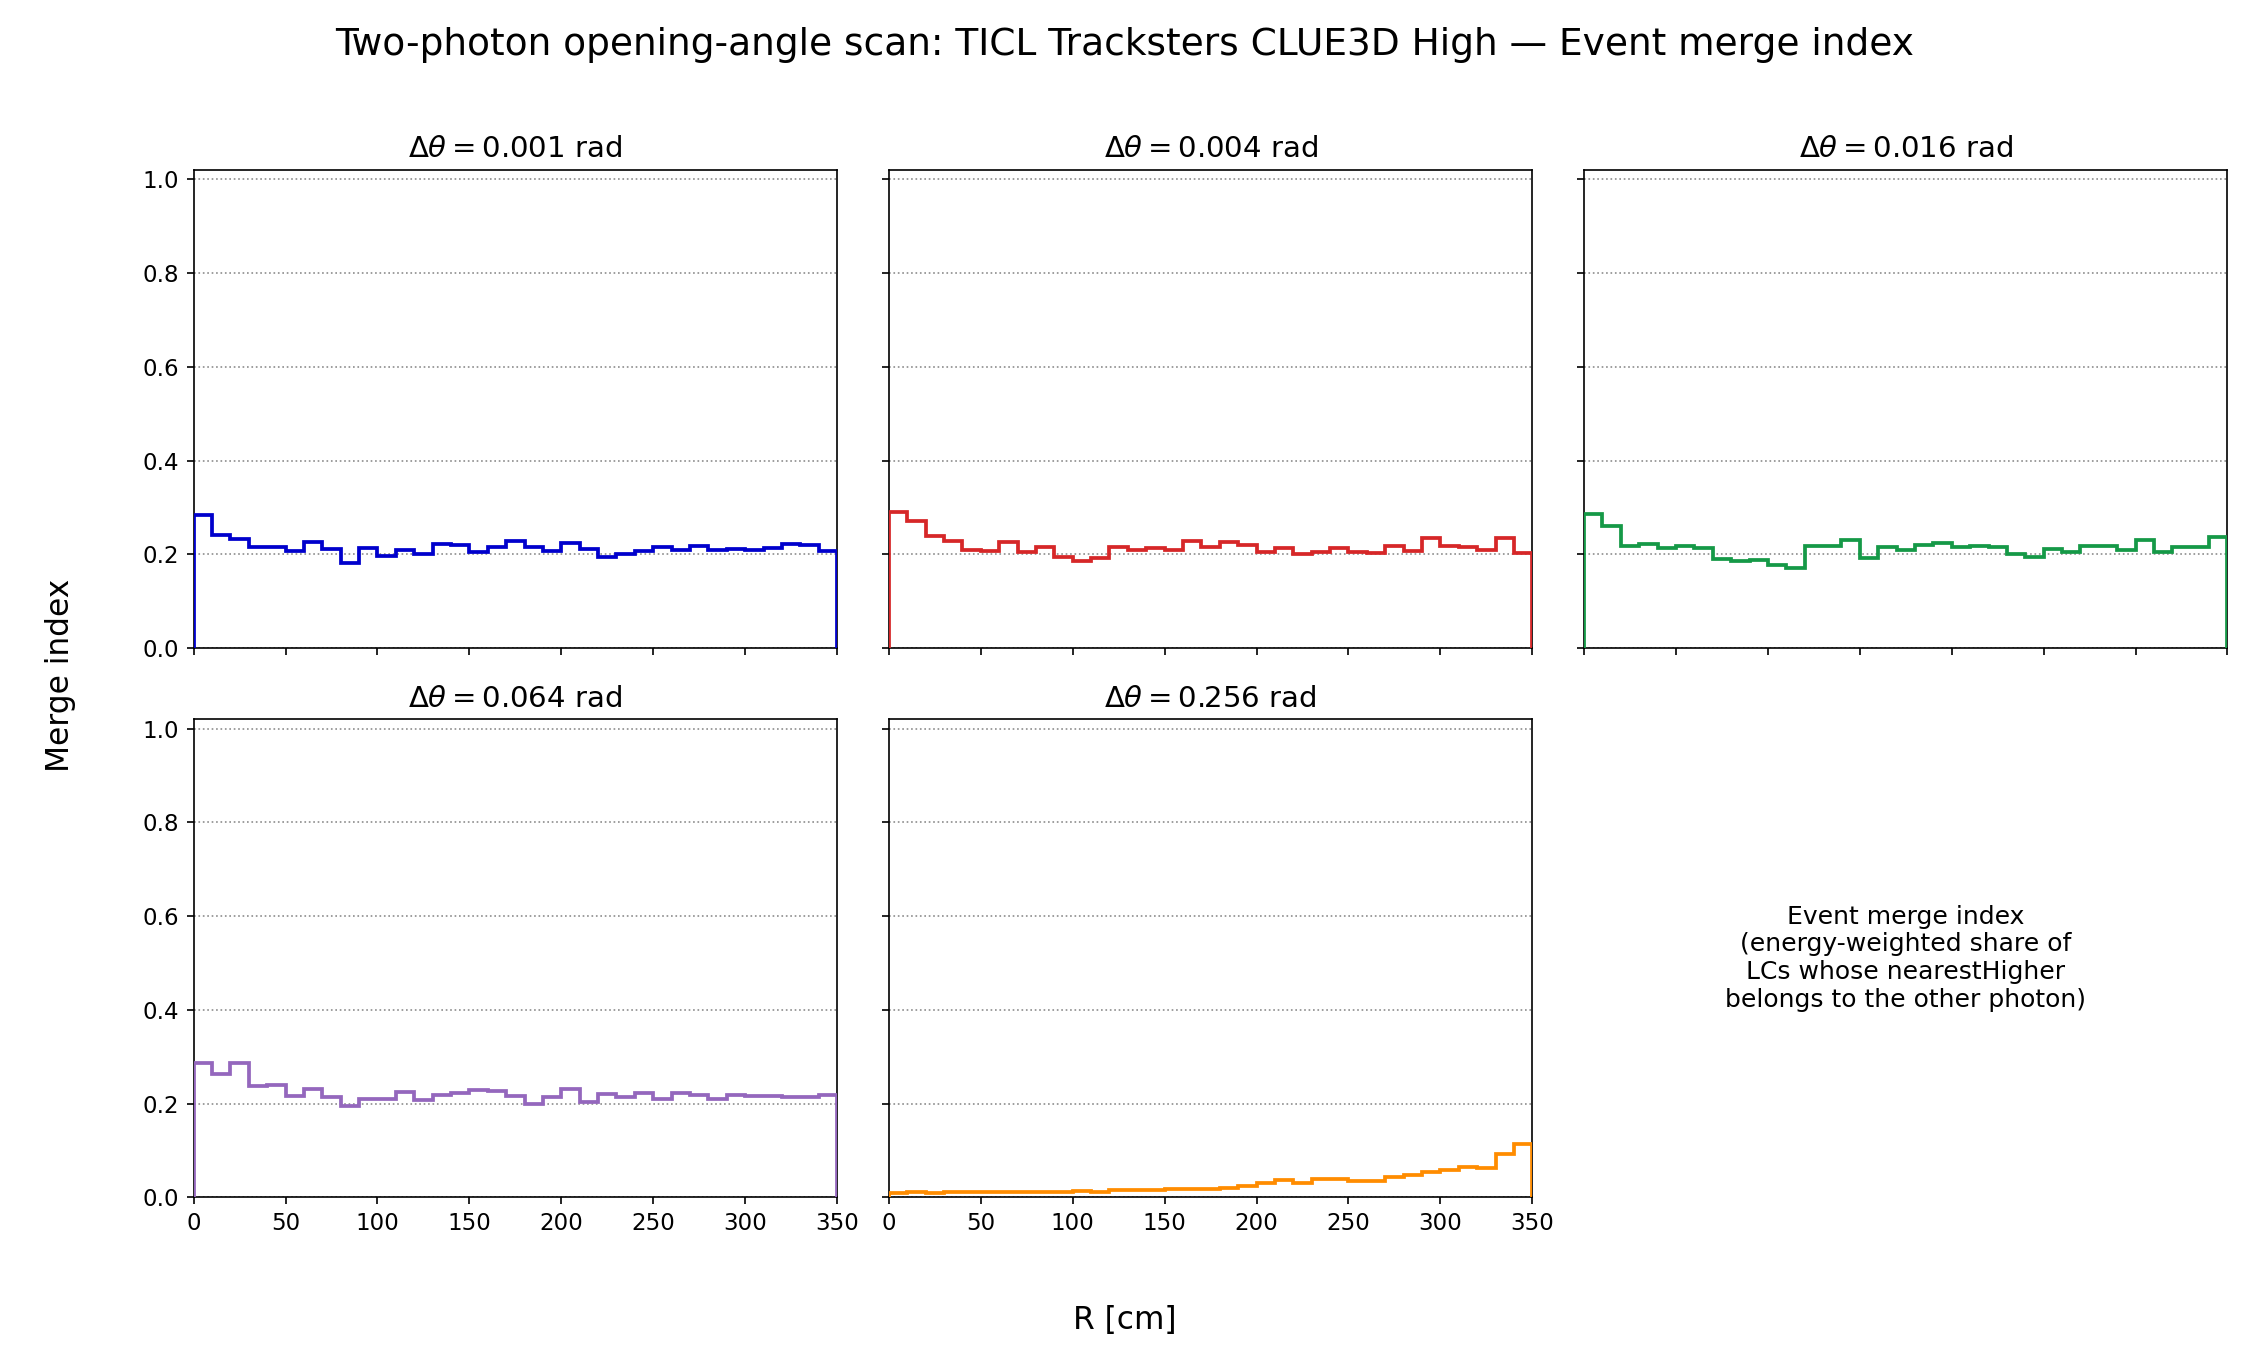
\includegraphics[width=0.86\textwidth]{figures/merge_index_theta.png}
  \caption{Merge index for the two-photon opening-angle scan. The index uses
  Eq.~\eqref{eq:mergeindex}, pooling follower energies within each bin. The largest opening angle provides the clearest
  increase in cross-shower linking with displacement.}
  \label{fig:mergeindextheta}
\end{figure*}

The opening-angle scan gives a complementary result
(Fig.~\ref{fig:mergeindextheta}). For the four smaller angles, the link index
is already substantial and remains near $0.2$ over most of the displacement
range. At the largest angle, $0.256$~rad, it starts near zero and increases
at large $\R$. A geometrically better-separated pair can therefore also lose
separation as displacement grows. Together, these scans show why tuning must
consider both shower completeness and cross-shower links: recovering energy
in larger Tracksters alone is not sufficient.


\section{CLUE3D performance with pileup}
\label{sec:pileup}

Pileup introduces many nearby showers with a broad range of energies and
particle species. I studied samples with an average of 200 additional interactions per bunch
crossing (PU200), keeping two efficiencies apart: the efficiency of
reconstructing the injected signal photon, and the inclusive efficiency
measured over all selected in-time SimTracksters (signal plus pileup). This distinction is essential:
the signal-only curve tests the same displaced-photon topology in a busier
environment, whereas the inclusive curve also changes the population being
measured.

\subsection{Signal efficiency and the meaning of displacement}

\begin{figure}[!htbp]
  \centering
  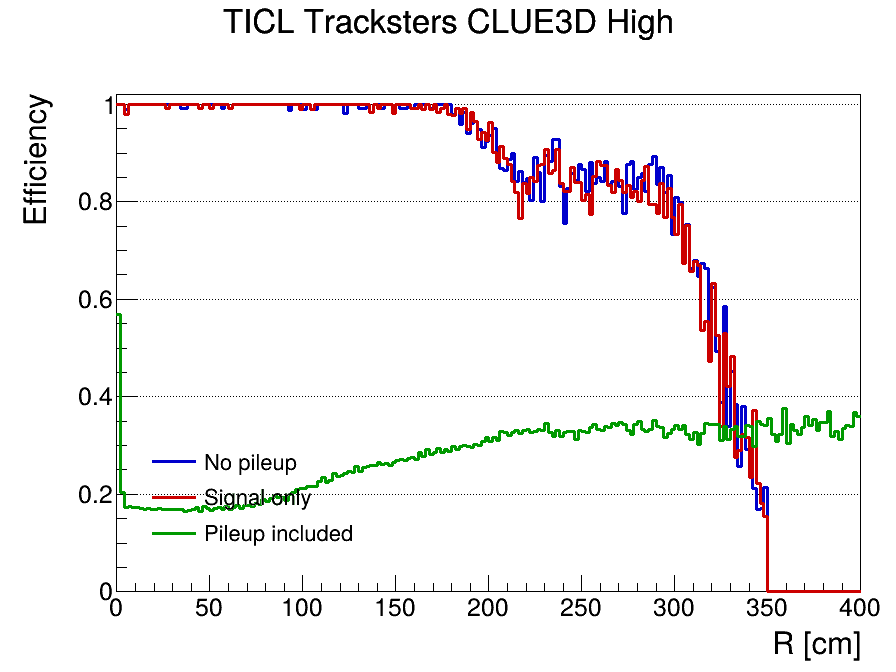
\includegraphics[width=\linewidth]{figures/pileup_efficiency.png}
  \caption{Default \cluethreed{} efficiency without pileup, for the generated
  signal photon in PU200, and for the inclusive in-time truth selection in
  PU200. The inclusive curve has a different denominator and a different
  interpretation of resolved $\R$ for charged particles.}
  \label{fig:pileupefficiency}
\end{figure}

Figure~\ref{fig:pileupefficiency} compares the no-pileup photon sample, the
signal photon in PU200, and the inclusive PU200 selection. The first two
curves are similar: both retain high efficiency at small displacement and
show the large-$\R$ degradation identified in
Section~\ref{sec:singlephoton}. The inclusive curve is quite different, and it
is dominated by pileup: the signal photon accounts for fewer than $1$ in
$1000$ of the selected in-time SimTracksters, so the inclusive denominator is
essentially the pileup population rather than the injected photon. It
falls sharply just outside the first displacement bin, reaches a minimum,
and then increases over a broad range of $\R$. This shape cannot be read as
the response to a single photon displaced progressively farther from the
beamline. A comparison of the Trackster and TICL-candidate efficiencies also
showed no substantial change in this behaviour at the candidate stage.

For pileup particles, resolved $\R$ is particularly easy to misinterpret. The
boundary position and direction define a line that can be extrapolated to
$z=0$. Charged particles bend in the magnetic field, so this line is a tangent
to a curved trajectory. Its intercept can be far from the beamline even when
the particle was produced close to it. A large resolved $\R$ in pileup is
therefore not evidence for a physically displaced production vertex. The
reconstruction consequences, however, are the same either way: a trajectory
with a large intercept still projects poorly onto the interaction point, so by
Eq.~\eqref{eq:displacedscale} its LayerClusters are pushed apart as
$d_{XY}\simeq\R|\Delta z|/z$ and suffer the same fragmentation as a genuinely
displaced shower.

Even for a straight photon trajectory, the longitudinal spread of collision
vertices matters. For a photon produced on the beamline at $z=z_v$, the
transverse intercept of its line at $z=0$ has magnitude
\begin{equation}
 R=|z_v|\tan\theta,
 \label{eq:pileupphotonR}
\end{equation}
where $\theta$ is the momentum polar angle relative to the beam axis, taking
the corresponding acute angle in either endcap. It is not the same experiment as
varying the transverse production offset of the displaced gun.

\subsection{Separating particle composition from reconstruction effects}

To investigate the inclusive shape, I broke the efficiency down per particle
in a 20\,000-event study, so that numerator and denominator could be examined
in the same kinematic slices.

\begin{figure*}[!tp]
  \centering
  \begin{subfigure}{0.49\textwidth}
    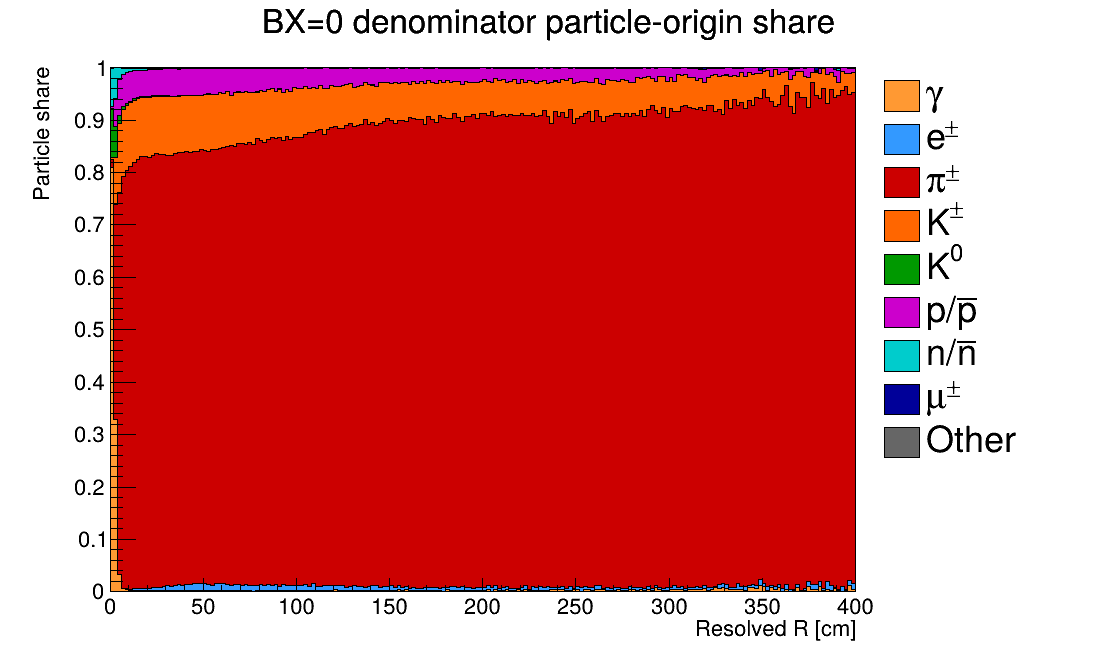
\includegraphics[width=\linewidth]{figures/pileup_composition.png}
    \caption{Composition of the in-time truth denominator.}
  \end{subfigure}\hfill
  \begin{subfigure}{0.49\textwidth}
    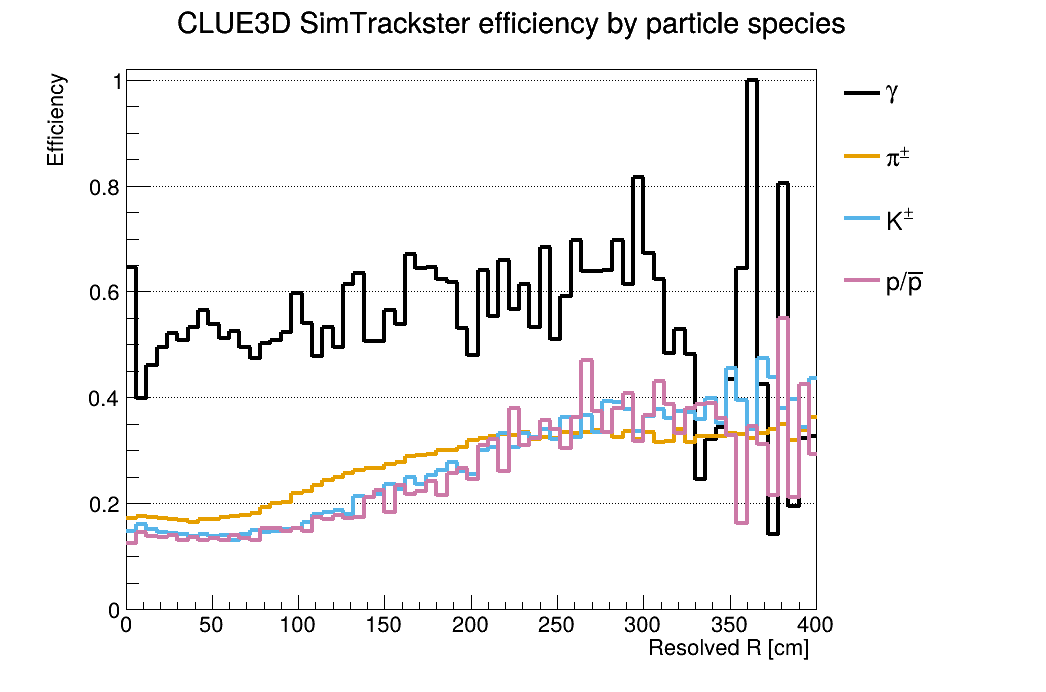
\includegraphics[width=\linewidth]{figures/pileup_efficiency_pid.png}
    \caption{Efficiency split by particle species.}
  \end{subfigure}
  \caption{Particle composition and reconstruction efficiency versus resolved
  $\R$ in pileup. The changing mixture contributes to the inclusive curve,
  but does not explain the displacement dependence within each species.}
  \label{fig:pileuppid}
\end{figure*}

The truth composition changes rapidly near $\R=0$. Photons contribute
strongly in the first bins, while charged pions dominate most of the larger
resolved-displacement range (Fig.~\ref{fig:pileuppid}). This accounts for part
of the inclusive change, but it is not a complete explanation: efficiencies
within individual species still depend on $\R$. Photon efficiency falls,
whereas the charged-hadron curves tend to rise. The remaining investigation
therefore treats these populations separately.

\begin{figure}[!htbp]
  \centering
  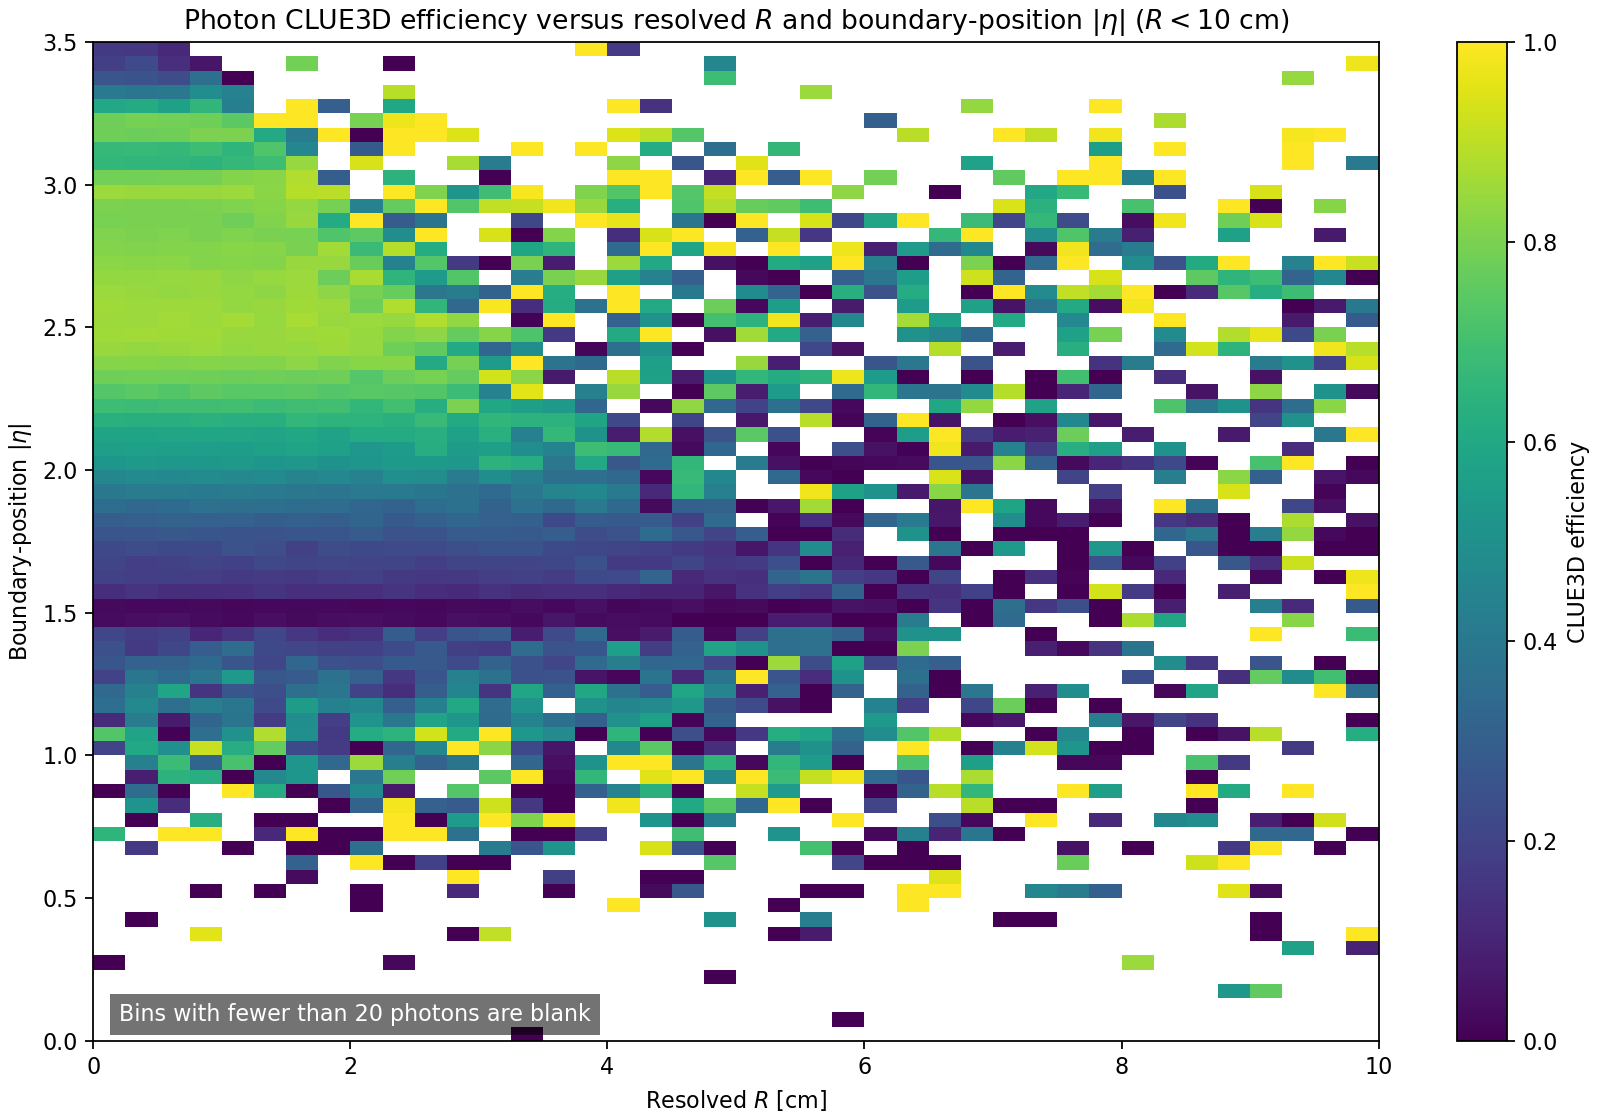
\includegraphics[width=\linewidth]{figures/pileup_photon_eta.png}
  \caption{Pileup-photon efficiency versus resolved $\R$ and boundary-position
  $|\eta|$ near the origin. Bins containing fewer than 20 photons are blank.
  The prominent angular structure motivates separating acceptance and
  kinematic effects from a dependence on displacement.}
  \label{fig:pileupphotoneta}
\end{figure}

For photons, the loss near the origin is concentrated in the low-energy
population, below about 2~GeV. The remaining dependence is really angular, not
on displacement. Pileup photons come from vertices close to the beamline, so
$z_v$ is small and Eq.~\eqref{eq:pileupphotonR} makes resolved
$\R=|z_v|\tan\theta$ essentially a proxy for the polar angle: a small increase
in $\R$ means a larger $\theta$ and hence a rapidly falling $|\eta|$. The
two-dimensional efficiency in Fig.~\ref{fig:pileupphotoneta} confirms this---the
structure runs in $|\eta|$ rather than in $\R$, with the loss confined to the
lower-$|\eta|$ edge of the HGCAL acceptance, where reconstruction is expected to
degrade. A
one-dimensional photon-versus-$\R$ curve therefore inherits this acceptance
edge and only looks like a displacement effect.

\subsection{Charged showers and LayerCluster multiplicity}

\begin{figure*}[!tp]
  \centering
  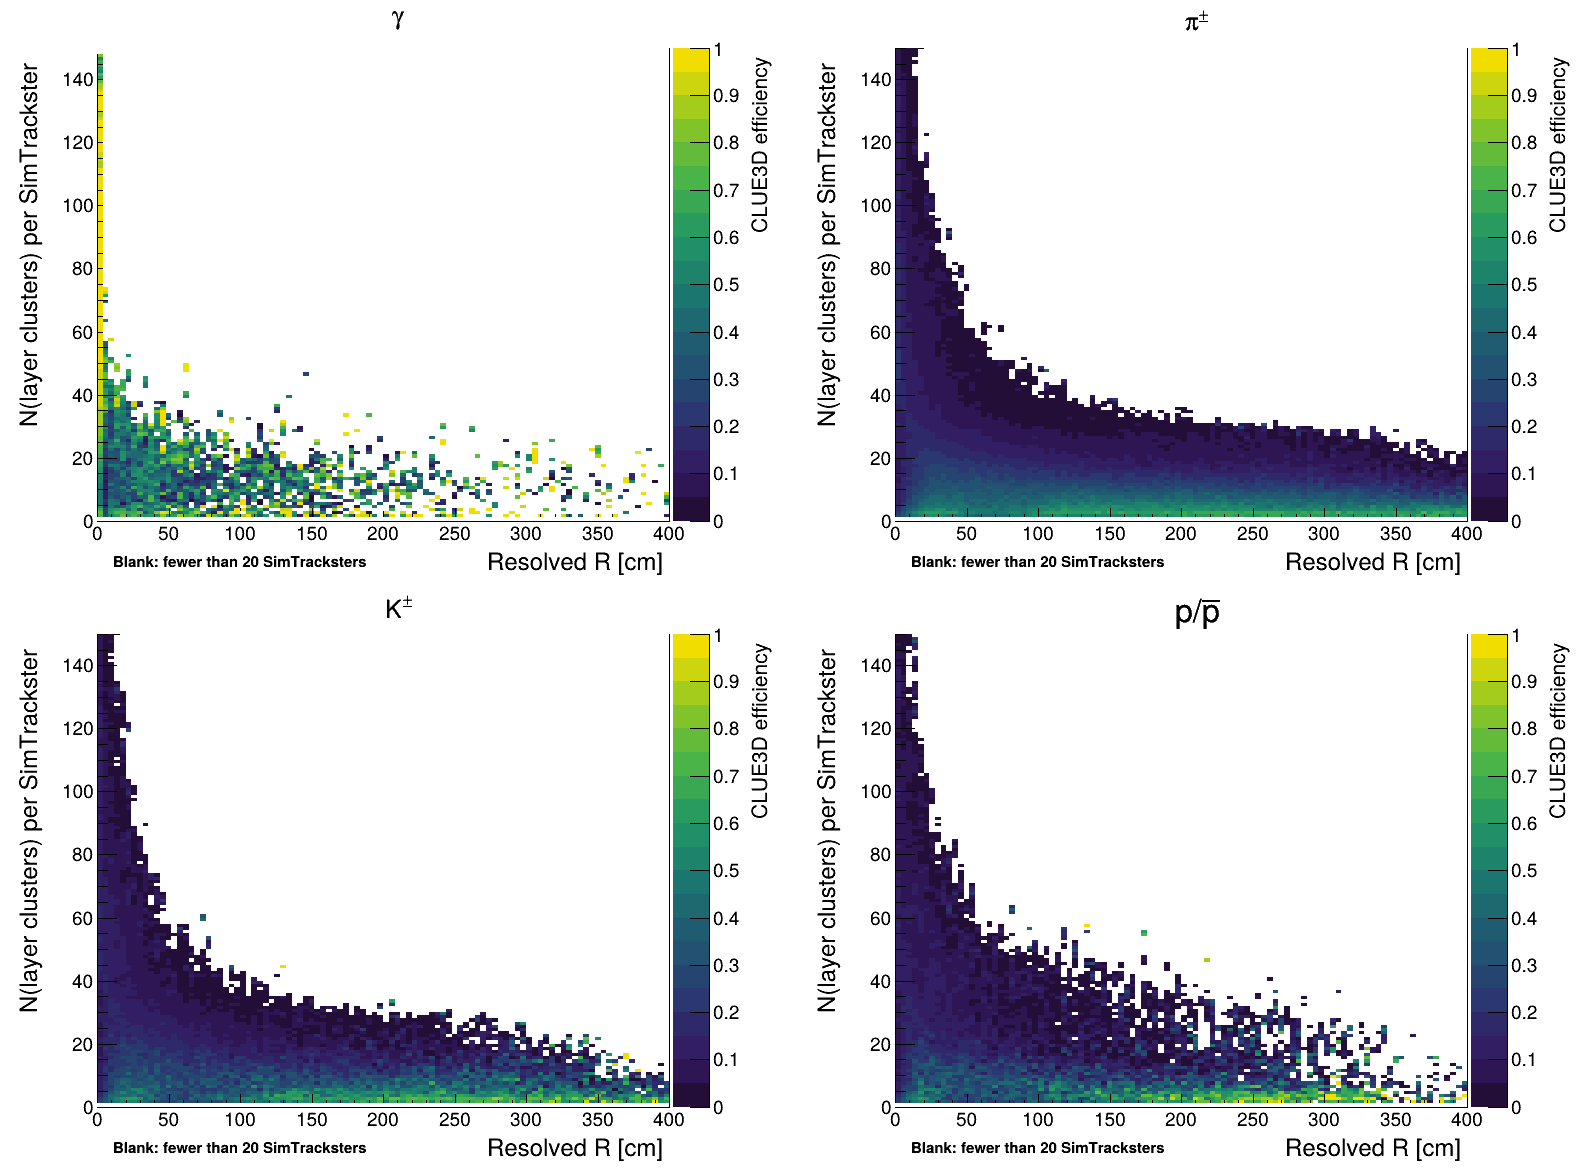
\includegraphics[width=0.9\textwidth]{figures/pileup_efficiency_lcs.png}
  \caption{Efficiency in bins of resolved $\R$ and truth-shower LC
  multiplicity, separated by particle species. The charged-hadron panels
  show lower efficiency for larger LC multiplicities and fewer large showers
  at large resolved $\R$. Blank bins contain fewer than 20 SimTracksters.}
  \label{fig:pileupshowersize}
\end{figure*}

For charged pions, kaons and protons the efficiency instead \emph{rises} with
resolved $\R$, the opposite of the photon trend, and the controlling variable
is the number of LCs in the truth shower: showers with many LCs rarely have
more than half of their energy collected in a single Trackster
(Fig.~\ref{fig:pileupshowersize}). As $\R$ grows, the whole pion
LC-multiplicity distribution shifts downward---not just its tail---so the
population moves towards smaller showers, and the charged-particle efficiency
rises with it.

Higher-momentum hadrons bend less, so they keep a smaller resolved intercept $\R$ while also developing
larger, higher-multiplicity showers; larger $\R$ therefore preferentially
selects the lower-energy, few-LC showers that \cluethreed{} reconstructs more
easily. This is a selection effect on the pileup population, not a direct
action of transverse displacement.

As an aside, similar connection first appeared the other way around. In
two-dimensional $(\R,\text{energy})$ and $(\R,|\eta|)$ efficiency maps for
pions, bins containing more reconstructed objects tended to have lower
efficiency. The natural guess was local crowding: that such showers sat in
busier neighbourhoods, where a high density of nearby reconstructed objects
might merge activity or otherwise disrupt the clustering. When I measured this
directly, however, efficiency showed no dependence on the number of
reconstructed objects in a shower's own neighbourhood, even at fixed $\R$,
energy and $|\eta|$.

Anyways, inclusive pileup efficiency must be
read together with particle identity, energy, angle and shower size, and the
signal-only selection remains the direct test of displaced-photon
reconstruction in pileup.

\section{Comparison with \cluestering{}}
\label{sec:cluestering}

\cluestering{} is a generalized, heterogeneous implementation of the CLUE
approach, with configurable coordinates and distance metrics. It retains the
density, nearest-higher and seed--follower structure introduced in
Section~\ref{sec:clue3d}, while allowing the neighbourhood geometry to be
changed. My work was to run and diagnose its application to displaced showers
in CMSSW, comparing several configurations with default \cluethreed{}.
The framework can use Cartesian positions directly or projective coordinates;
removing the origin assumption is therefore one possibility, rather than a
defining property of \cluestering{}.

\subsection{Cartesian distance metrics}

For Cartesian coordinates $(x,y,z)$, I explored three familiar distance
families. Writing $\Delta x=x_i-x_j$, and similarly for $y$ and $z$, their
unweighted forms are
\begin{align}
 D_2 &= \sqrt{\Delta x^2+\Delta y^2+\Delta z^2},\\
 D_1 &= |\Delta x|+|\Delta y|+|\Delta z|,\\
 D_\infty &= \max(|\Delta x|,|\Delta y|,|\Delta z|).
\end{align}
Euclidean distance $D_2$ measures straight-line separation, so a fixed distance
cut selects a sphere. Manhattan distance $D_1$ adds the separations along the
three axes and selects an octahedron. Chebyshev distance $D_\infty$ takes the
largest component and selects a cube: all three coordinate differences must
individually lie within the cut. These shapes give different neighbours even
when the numerical distance setting is identical.

Weights allow the longitudinal and transverse reaches to be adjusted. With
positive weights $w_k$ and coordinate differences $\Delta x_k$, the corresponding
forms are
\begin{align}
 D_{2,w} &= \sqrt{\sum_k w_k(\Delta x_k)^2},\\
 D_{1,w} &= \sum_k w_k|\Delta x_k|,\\
 D_{\infty,w} &= \max_k\bigl(w_k|\Delta x_k|\bigr).
\end{align}
The weighted examples shown below use $(w_x,w_y,w_z)=(1,1,2)$ for Euclidean
and Chebyshev distance; the Manhattan example is unweighted. Increasing the
longitudinal weight shortens the allowed reach in $z$. In these conventions,
a weight of two reduces the pure longitudinal reach by $\sqrt{2}$ for
Euclidean distance and by two for Chebyshev distance. All these Cartesian
metrics depend only on coordinate differences and make no projection towards
the interaction point.

\subsection{A projective metric under development}

I also tested a work-in-progress projective configuration, labelled
\emph{Gnomonic} in the plots. It maps LC positions to the direction coordinates
\begin{equation}
 \mathbf{g}=\left(\frac{x}{|z|},\frac{y}{|z|}\right),
\end{equation}
and uses the layer index $\ell$ as the longitudinal coordinate. Within one
endcap, the tested cylinder distance is
\begin{equation}
 D_{\mathrm{cyl}}(i,j)=\max\!\left(
 \frac{|\mathbf{g}_i-\mathbf{g}_j|}{\sigma_T},
 \frac{|\ell_i-\ell_j|}{L}\right).
 \label{eq:cluesteringcylinder}
\end{equation}
A cut $D_{\mathrm{cyl}}<d$ selects a transverse disc of radius $d\sigma_T$
and a longitudinal interval of half-height $dL$: a cylinder in the transformed
coordinate space. The transverse and longitudinal scales can thus be set
separately. Points on an ideal pointing shower have constant $\mathbf{g}$;
non-pointing showers drift across this plane, so some degradation with
displacement is still expected.

The tested implementation clusters only the electromagnetic section (EE).
It uses $\sigma_T=0.003$, $L=4$ layers, density radius $d_c=1$, seed distance
2.8 and outlier distance 3.6, with the distances expressed in the normalized
units of Eq.~\eqref{eq:cluesteringcylinder}, not centimetres. To account for PU $\eta$-uniform density, density
threshold also varies with direction:
\begin{equation}
 \rho_c(\mathbf{g})=\SI{0.8}{GeV}
       \left(\frac{0.42}{|\mathbf{g}|}\right)^2.
\end{equation}

\subsection{First comparisons without pileup}

These comparisons are exploratory tests of a few metrics and parameter
choices, not the result of tuning. For the Cartesian configurations,
I held the density radius at $d_c=5$~cm and the density threshold at
$\rho_c=6$~GeV, and concentrated on the nearest-higher distance $d_m$.
The preceding studies identified the distance reach as a particularly direct
control of fragmentation, making it the first parameter to vary before a
broader density-and-distance tuning. Unweighted and weighted Euclidean
metrics were tested at $d_m=3$ and 6~cm; Manhattan and weighted Chebyshev
are shown at 6~cm. Default parameters are used for \cluethreed{}, which is the baseline.

\begin{figure*}[!tp]
  \centering
  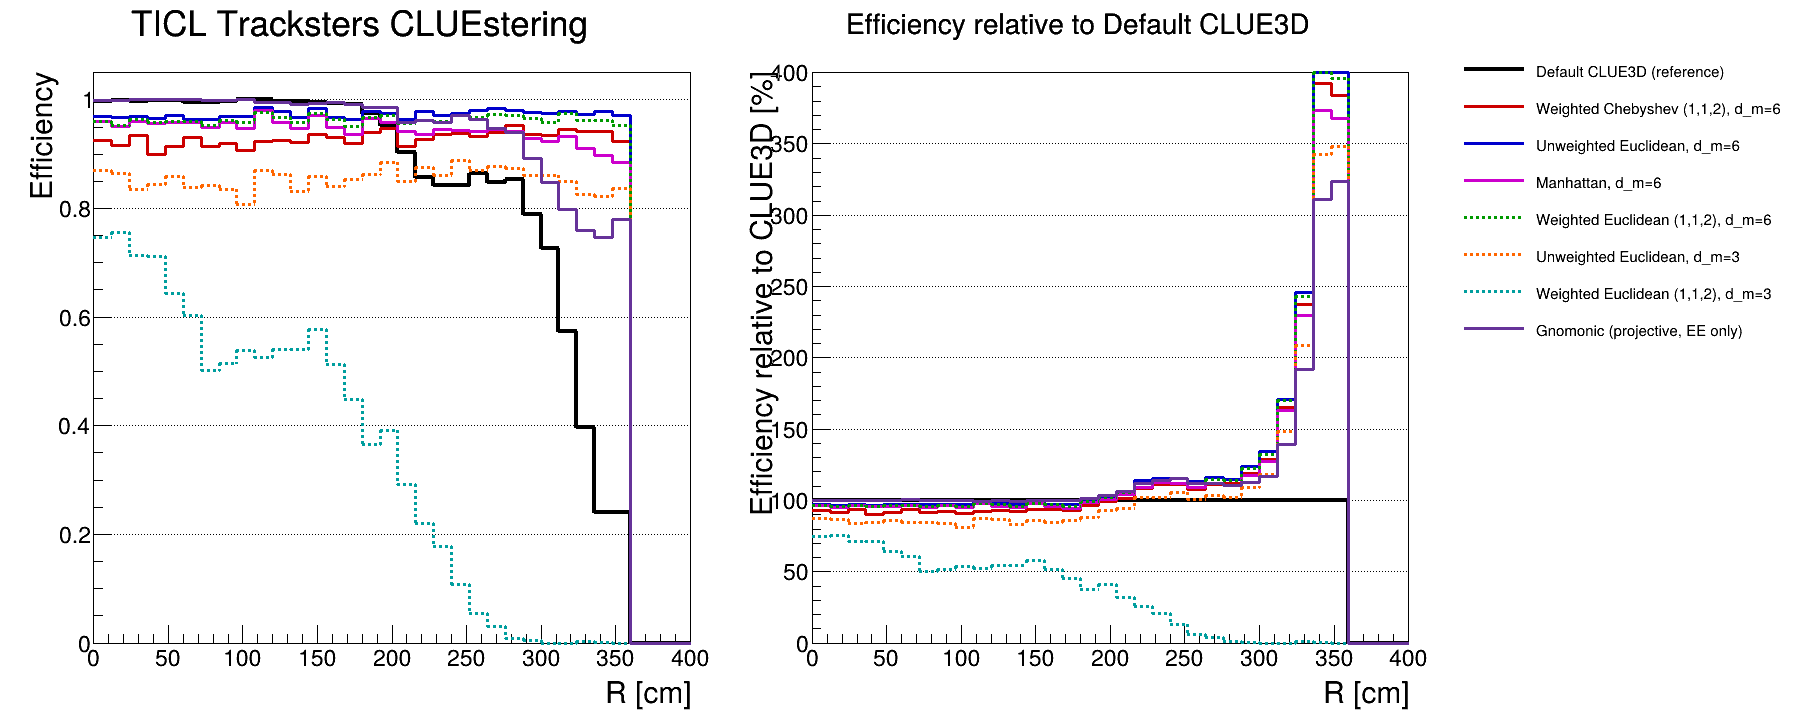
\includegraphics[width=\textwidth]{figures/cluestering_no_pu.png}
  \caption{Single-photon efficiency without pileup for the exploratory
  \cluestering{} configurations, including the EE-only gnomonic configuration,
  with default \cluethreed{} as the baseline. The right panel shows
  $100\,\epsilon/\epsilon_{\mathrm{CLUE3D}}$; $100\%$ denotes equal efficiency.
  The generated displacement scan ends at 350~cm.}
  \label{fig:cluesteringefficiencies}
\end{figure*}

The no-pileup comparison uses 20\,000 generated single-photon events with
energies of 10--250~GeV and $\R=0$--350~cm in Run4D121 geometry, subject to
the gun's surface-acceptance requirements. Figure~\ref{fig:cluesteringefficiencies}
shows that the 6~cm Cartesian configurations largely avoid the severe
large-displacement loss of \cluethreed{}. The two Euclidean variants retain
efficiencies in the mid-to-high $90\%$ range over most of the scan; Manhattan
and weighted Chebyshev also remain efficient, with somewhat lower curves.
These simple choices already show that the default \cluethreed{} behaviour
is not an unavoidable consequence of a displaced shower.

The gnomonic configuration performs well near the origin and degrades at
large displacement, as expected for projective coordinates. Its decline is
much less severe than that of \cluethreed{}, however, so this first test also
looks promising. Sharing an origin projection does not imply identical
performance: the cylinder neighbourhood, distance scales and density
prescription differ from those of \cluethreed{}.

The surprise is the smaller Euclidean distance setting. Unweighted Euclidean
at 3~cm is less efficient than at 6~cm, while the weighted 3~cm configuration
loses almost all efficiency by approximately 300~cm. Since it uses Cartesian
coordinates, this failure cannot be attributed to an origin projection.

\subsection{Understanding the weighted Euclidean 3 cm failure}

\begin{figure*}[!tp]
  \centering
  \begin{subfigure}{0.49\textwidth}
    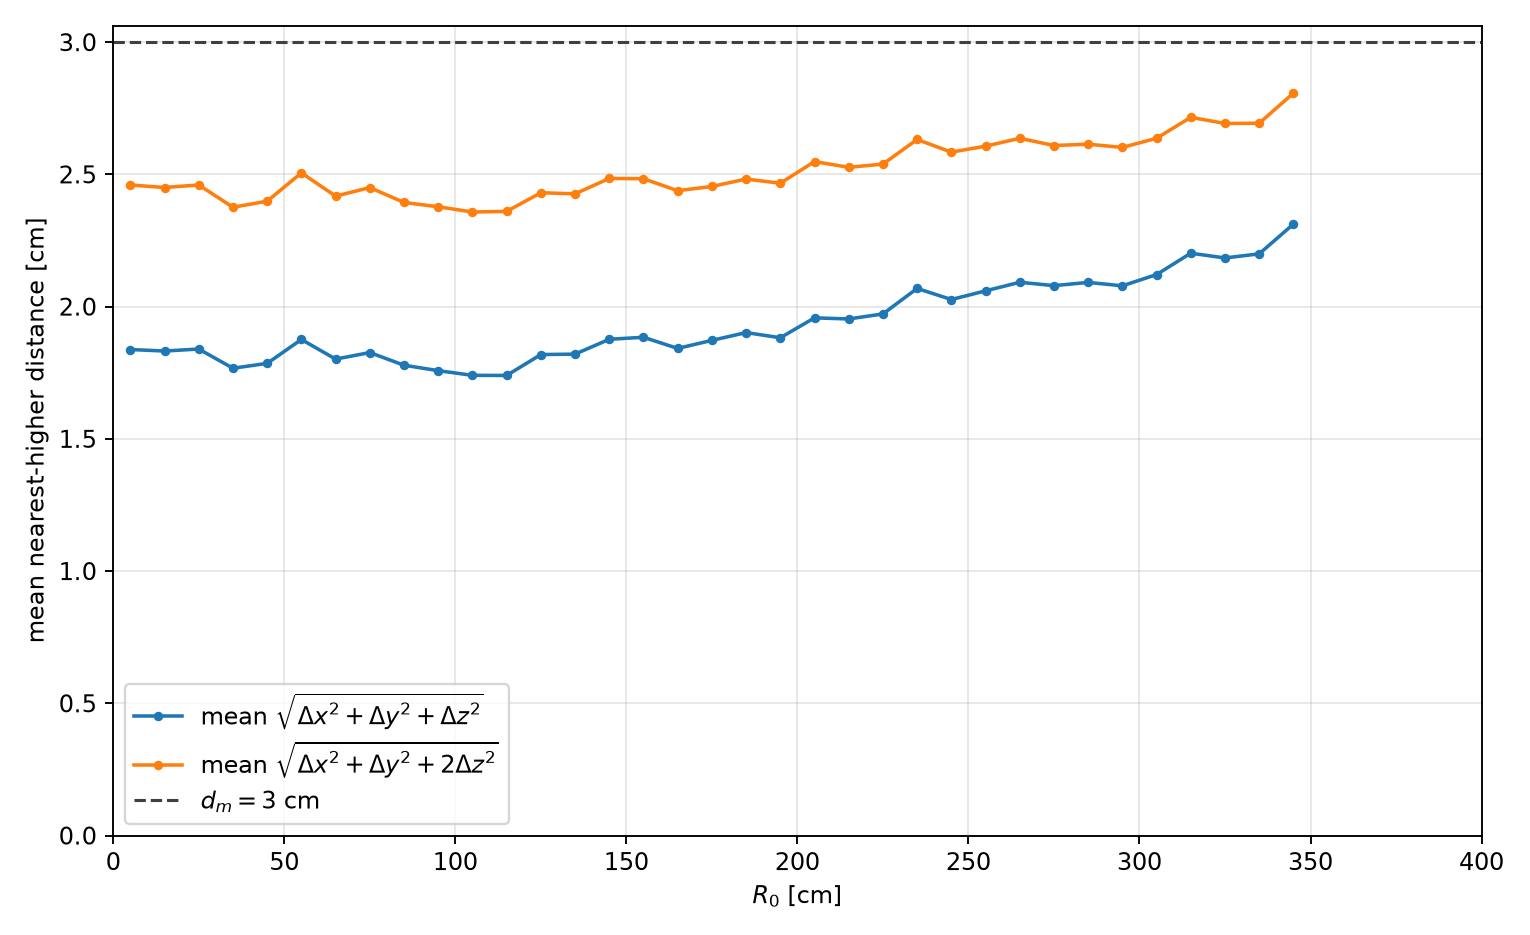
\includegraphics[width=\linewidth]{figures/cluestering_link_distances.png}
    \caption{Mean nearest-higher link distance, unweighted and weighted.}
  \end{subfigure}\hfill
  \begin{subfigure}{0.49\textwidth}
    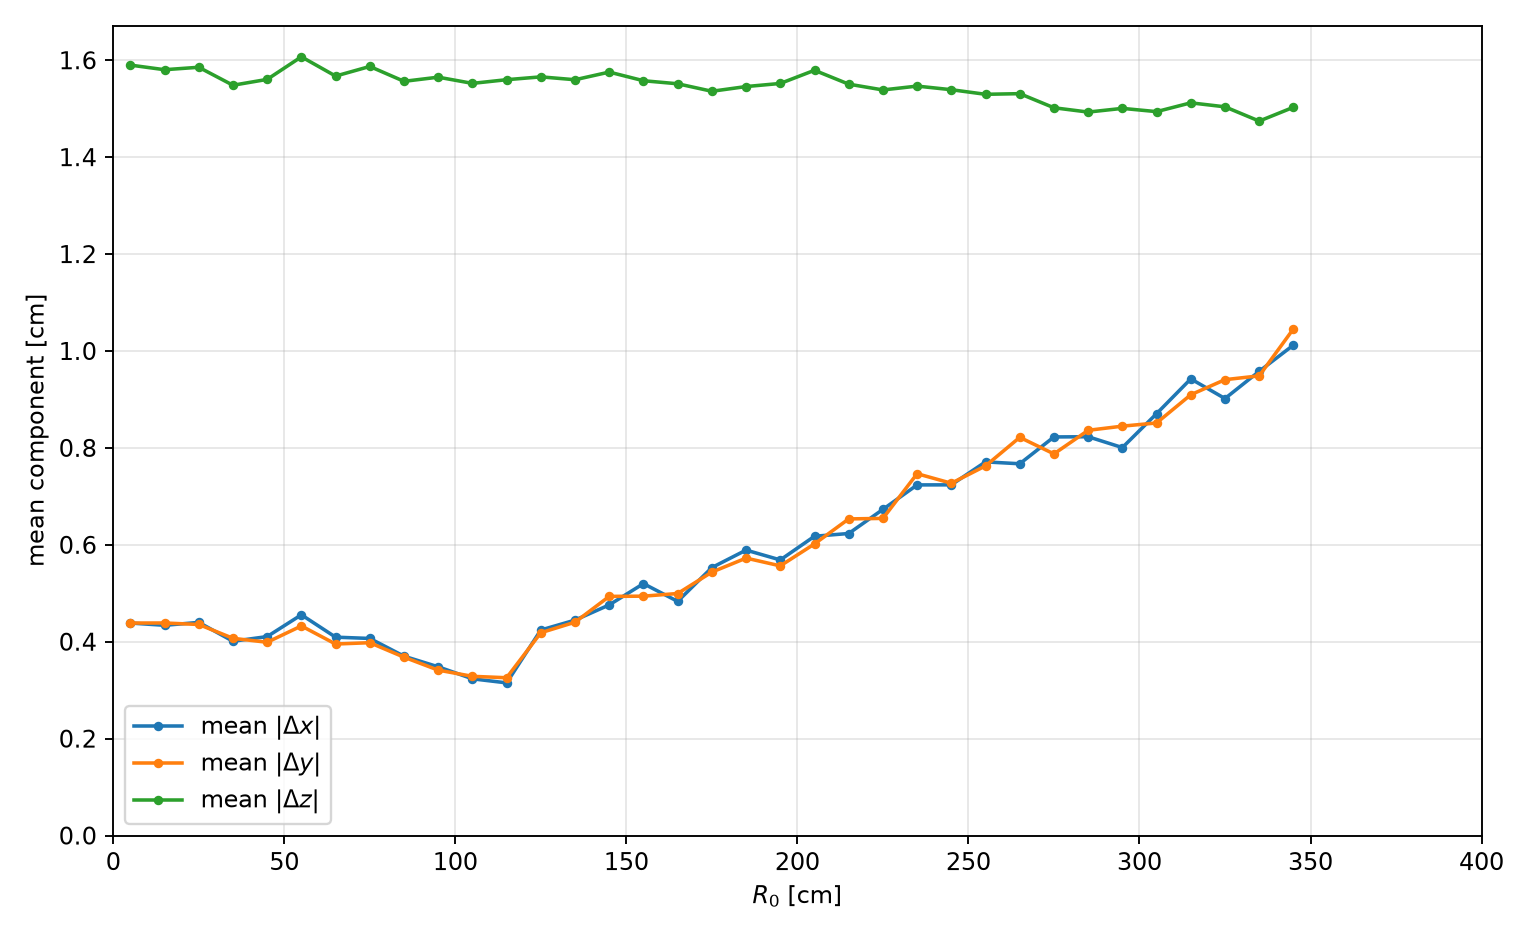
\includegraphics[width=\linewidth]{figures/cluestering_link_components.png}
    \caption{Mean absolute components of the nearest-higher link.}
  \end{subfigure}
  \par\medskip
  \begin{subfigure}{0.49\textwidth}
    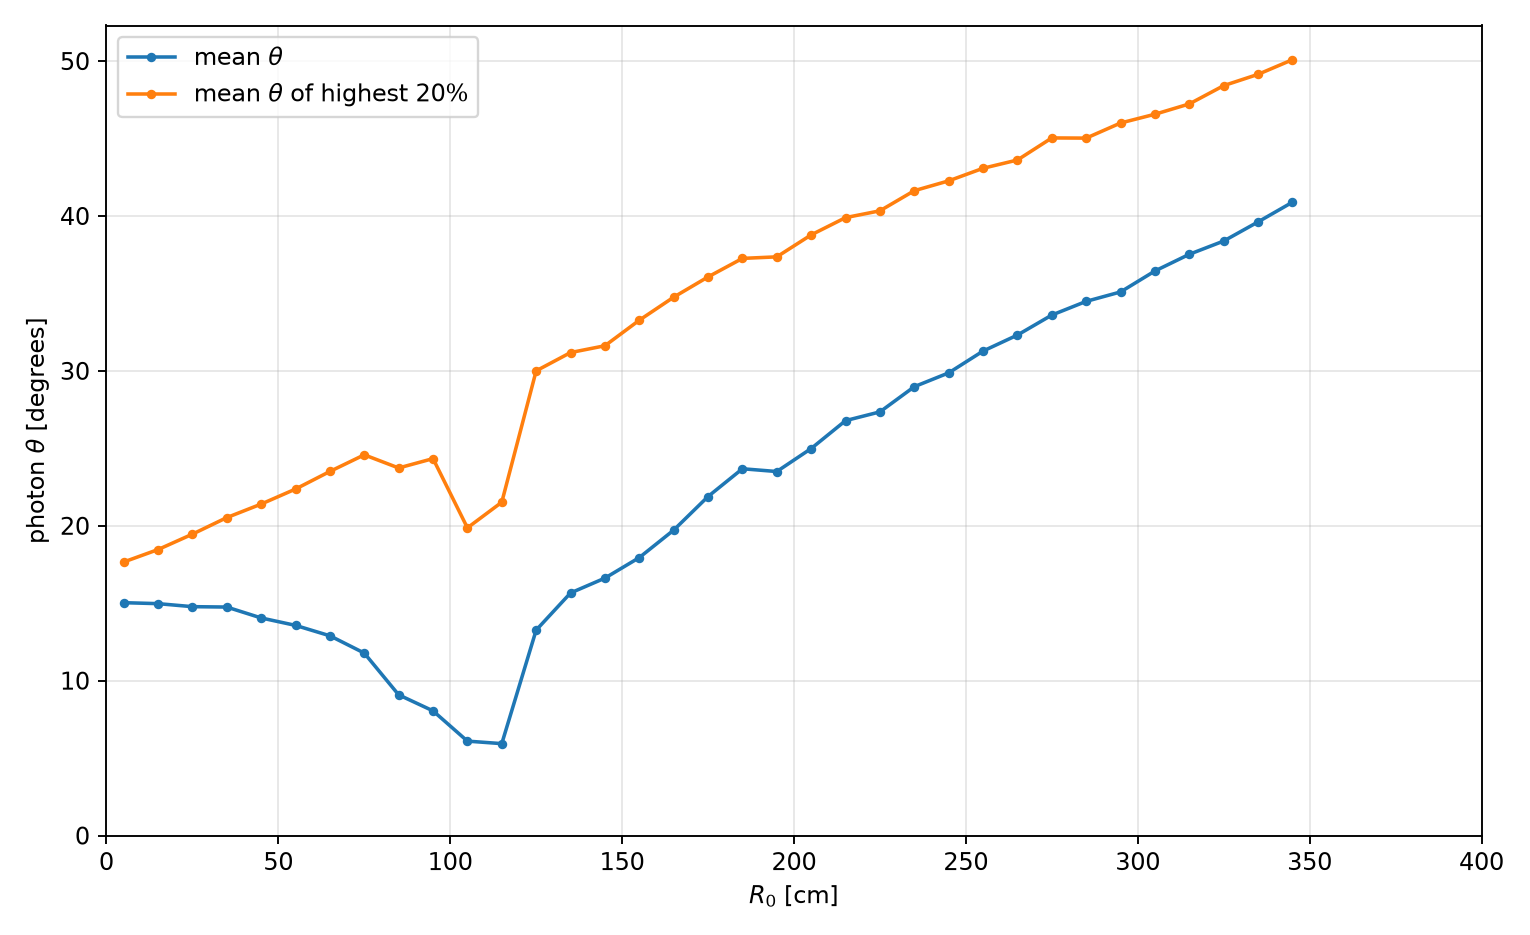
\includegraphics[width=\linewidth]{figures/cluestering_photon_theta.png}
    \caption{Mean photon angle $\theta$, and the mean of its most-inclined fifth.}
  \end{subfigure}\hfill
  \begin{subfigure}{0.49\textwidth}
    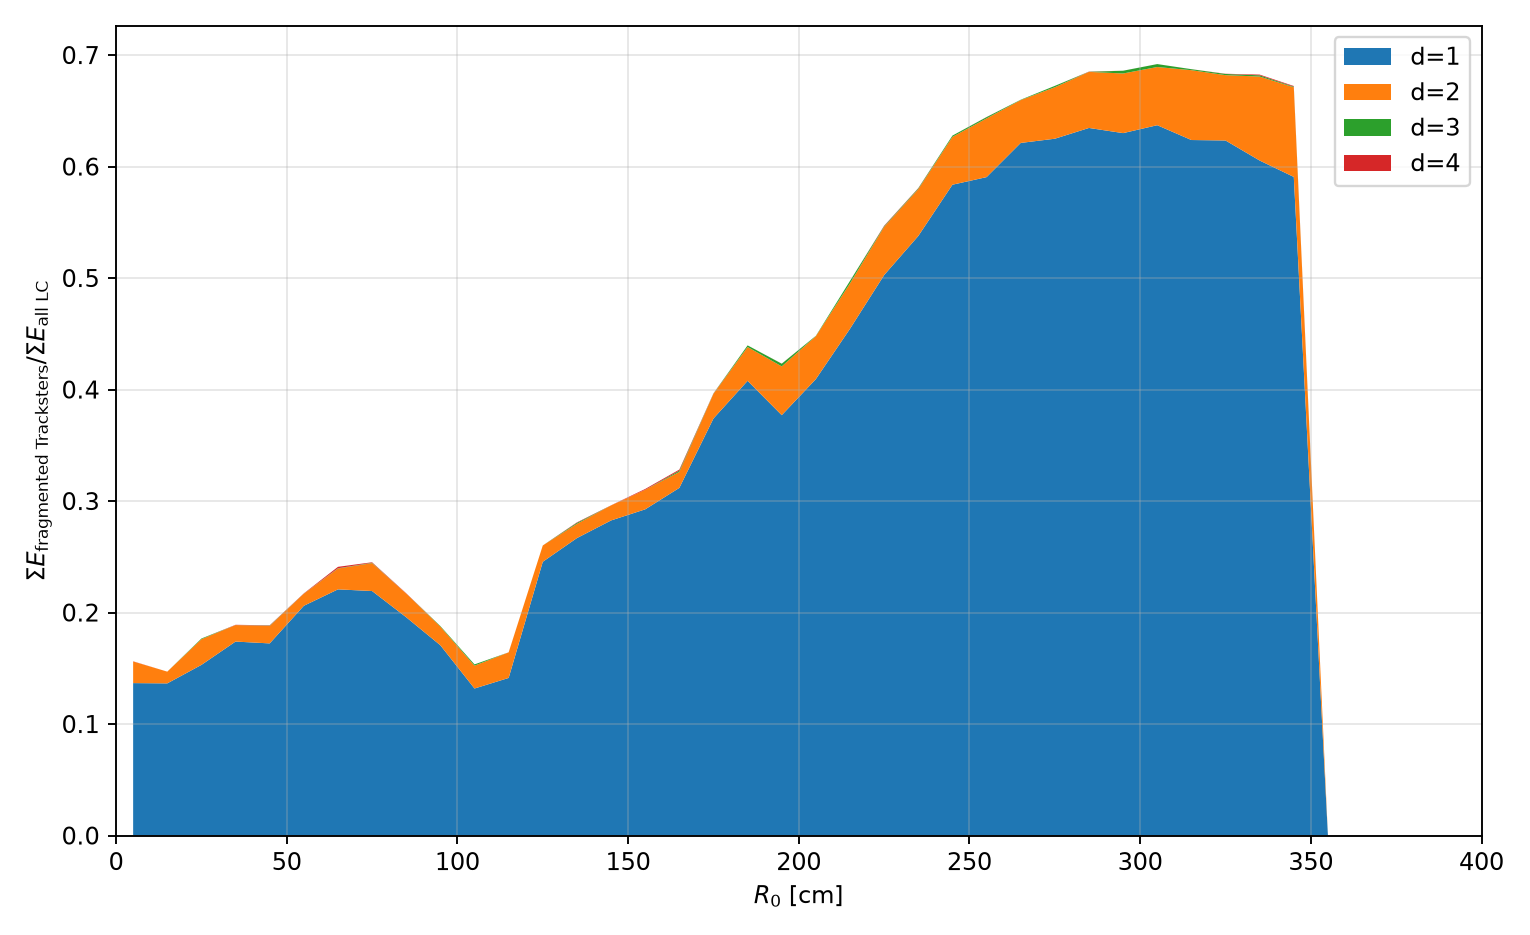
\includegraphics[width=\linewidth]{figures/cluestering_fragment_energy.png}
    \caption{Fraction of shower energy split into fragments, by the layer gap
    of the broken link.}
  \end{subfigure}
  \caption{Diagnostics for the weighted Euclidean metric at $d_m=3$~cm, versus
  truth displacement $R_0$. Panels (a) and (b) use only valid nearest-higher
  links. Panel (d) sums the full energy of the clusters rooted at seeds whose
  higher-density continuation lies beyond the 3~cm reach, normalized to the
  total LC energy; the label $d$ in its legend is the physical layer gap of the
  broken link.}
  \label{fig:cluesteringdiagnostic}
\end{figure*}

To understand why, I examined the nearest-higher links: their distance, their
separate coordinate components, and the shower energy that ends up in the
fragments they produce (Fig.~\ref{fig:cluesteringdiagnostic}). The links tell a
simple geometric story. An inclined shower advances along a tilted axis, so
consecutive layers are offset not only in $z$ but also transversely. For a
layer gap $\Delta z$, this transverse step is
\begin{equation}
 \Delta r_{xy}\simeq|\Delta z|\tan\theta,
 \label{eq:cluesteringangle}
\end{equation}
where $\theta$ is the photon polar angle. The HGCal layer spacing fixes the
longitudinal part of each link, while a larger inclination---which is what a
larger displacement produces---adds transverse distance. Panel~(b) shows
exactly this: at large $\R$ the transverse components grow while the
longitudinal one barely changes. Once the transverse step outgrows the 3~cm
reach, the link is cut and a single continuous shower is split---even though
nothing here projects towards the origin. The failure is therefore not really
inherent to displaced particles, but to particles with large $\theta$, which
displaced particles simply tend to have.

One thing looks paradoxical at first: the mean weighted link distance stays
below 3~cm across the whole scan (panel~a), yet the efficiency collapses. The
resolution is that clustering acts on individual links, and an average
comfortably under the threshold can still hide many links above it. The start
of the scan makes the point: below about 100~cm the mean photon angle and the
mean link distance both fall, yet the most inclined fifth of the photons moves
to larger $\theta$ (panel~c). It is this growing angular tail, not the average
shower, that runs into the distance limit.

The fragmentation diagnostic ties this link-level failure to the lost energy
(panel~d). The energy in clusters that hang off a seed whose higher-density
continuation lies beyond the reach rises to about two thirds of the total
shower energy at large displacement, dominated by continuations just one layer
away. A large part of each shower is therefore broken off into separate
objects. The lesson of the 3~cm test is that Cartesian coordinates remove the
artificial projective separation, but the distance reach and metric weights
must still be large enough to follow an inclined shower from one layer to the
next. This is a concrete target for future tuning.

\subsection{Performance in pileup}

The PU200 comparison uses a 10\,000-event sample for each tested
configuration. As in Section~\ref{sec:pileup}, I measured the generated signal
photon separately from the inclusive in-time truth population, and added two
complementary rates: signal-photon duplicates and reconstructed-object merges.
The signal measurement tests recovery of the displaced photon in a busy event;
the inclusive one tests the response to the many additional showers.

\begin{figure*}[!tp]
  \centering
  \begin{subfigure}{\textwidth}
    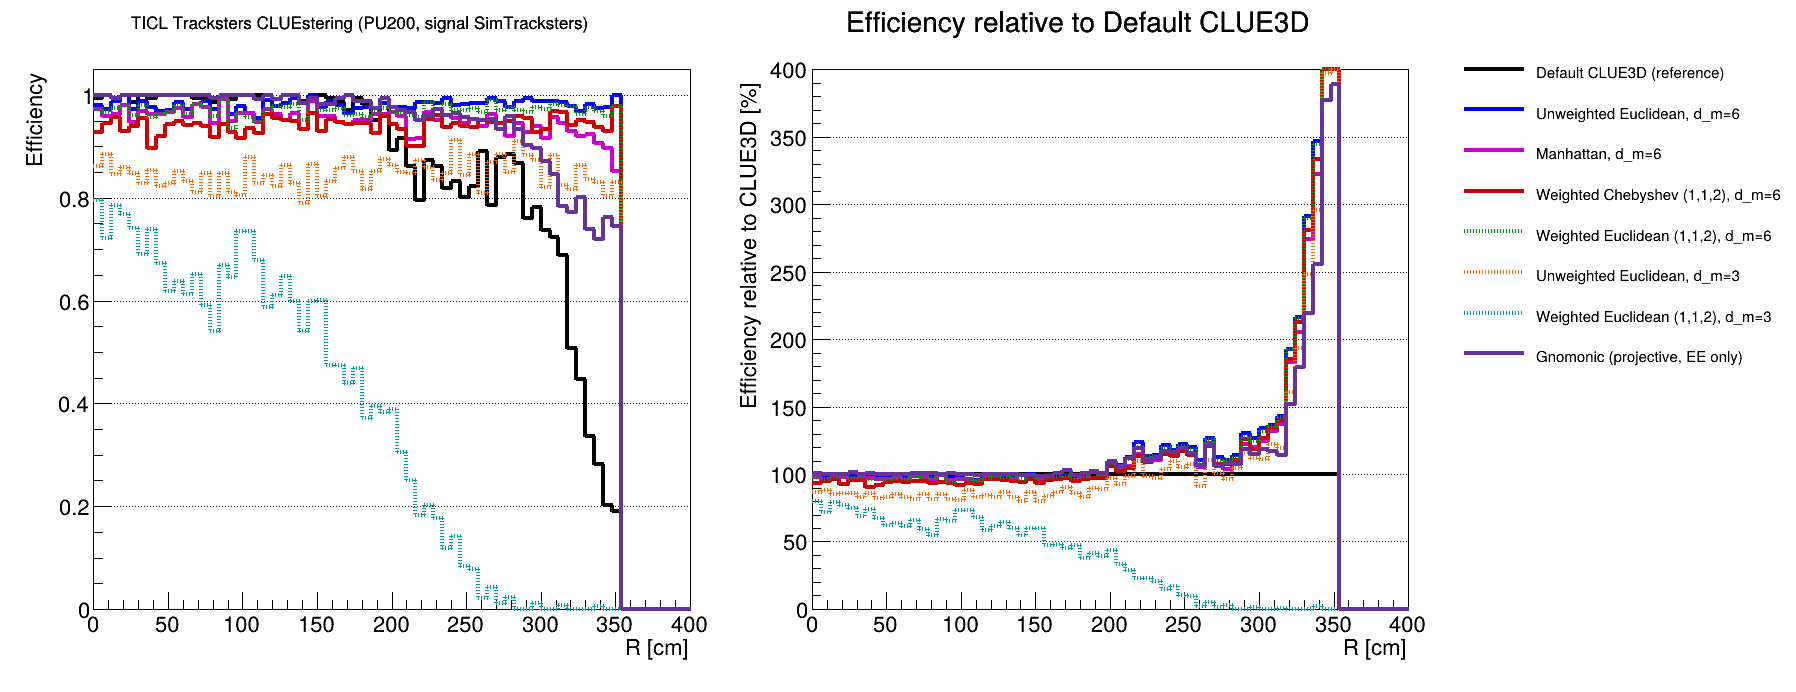
\includegraphics[width=\linewidth]{figures/cluestering_signal_pu.png}
    \caption{Efficiency for the generated signal photon in PU200.}
    \label{fig:cluesteringsignalpu}
  \end{subfigure}
  \par\medskip
  \begin{subfigure}{\textwidth}
    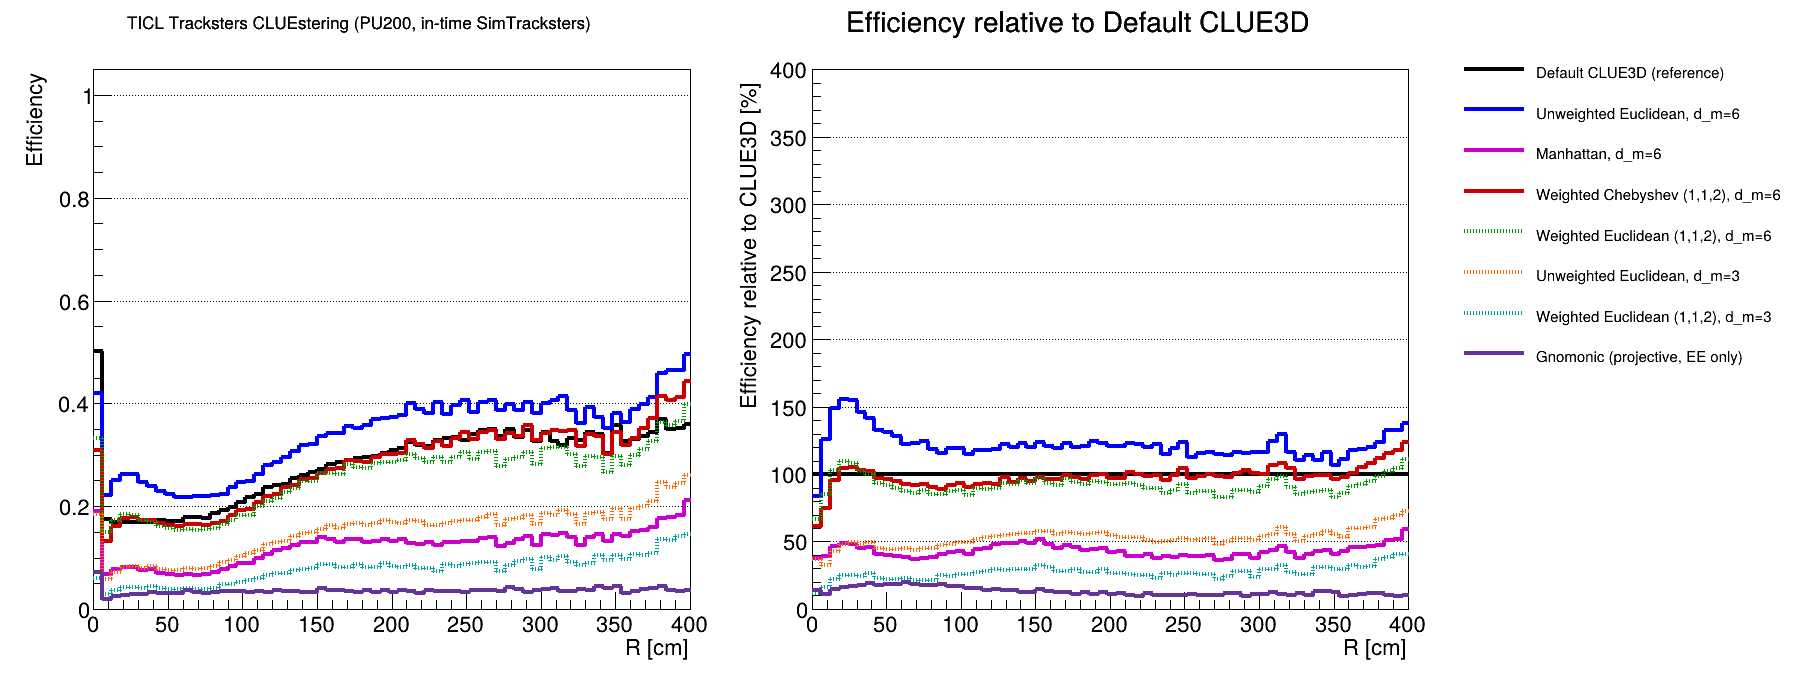
\includegraphics[width=\linewidth]{figures/cluestering_inclusive_pu.png}
    \caption{Efficiency for the inclusive in-time truth population.}
    \label{fig:cluesteringinclusive}
  \end{subfigure}
  \caption{PU200 efficiencies, with default \cluethreed{} as the baseline
  and the same relative-efficiency convention as
  Fig.~\ref{fig:cluesteringefficiencies}. The inclusive denominator includes
  showers in the hadronic sections, which the tested EE-only gnomonic
  configuration does not cluster.}
  \label{fig:cluesteringpuefficiencies}
\end{figure*}

For the signal photon, the no-pileup ordering survives
(Fig.~\ref{fig:cluesteringsignalpu}): the 6~cm Cartesian configurations stay
efficient across the scan, the gnomonic configuration again beats
\cluethreed{} at large displacement, and the weighted Euclidean 3~cm failure
is still present. Pileup does not remove the geometric limitations, nor does
it erase the gains of the more successful configurations.

The inclusive picture is different (Fig.~\ref{fig:cluesteringinclusive}). The
6~cm Cartesian metrics remain competitive---unweighted Euclidean improves on
\cluethreed{} over most of the range and weighted Chebyshev is broadly
comparable---while Manhattan and the 3~cm choices recover much less. The
gnomonic configuration is the striking outlier: even though its signal
efficiency is the \emph{higher} of the two, it collects only a small fraction
of the inclusive population, several times less than \cluethreed{} does.

This is unlikely to be the projective metric itself. We assume its direction-dependent
density threshold further suppresses much of the pileup, and it also hasn't been set up for hadronic subdetector which is relevant for PU. These are working
explanations rather than conclusions, confirming them requires further
checks.

\begin{figure*}[!tp]
  \centering
  \begin{subfigure}{0.49\textwidth}
    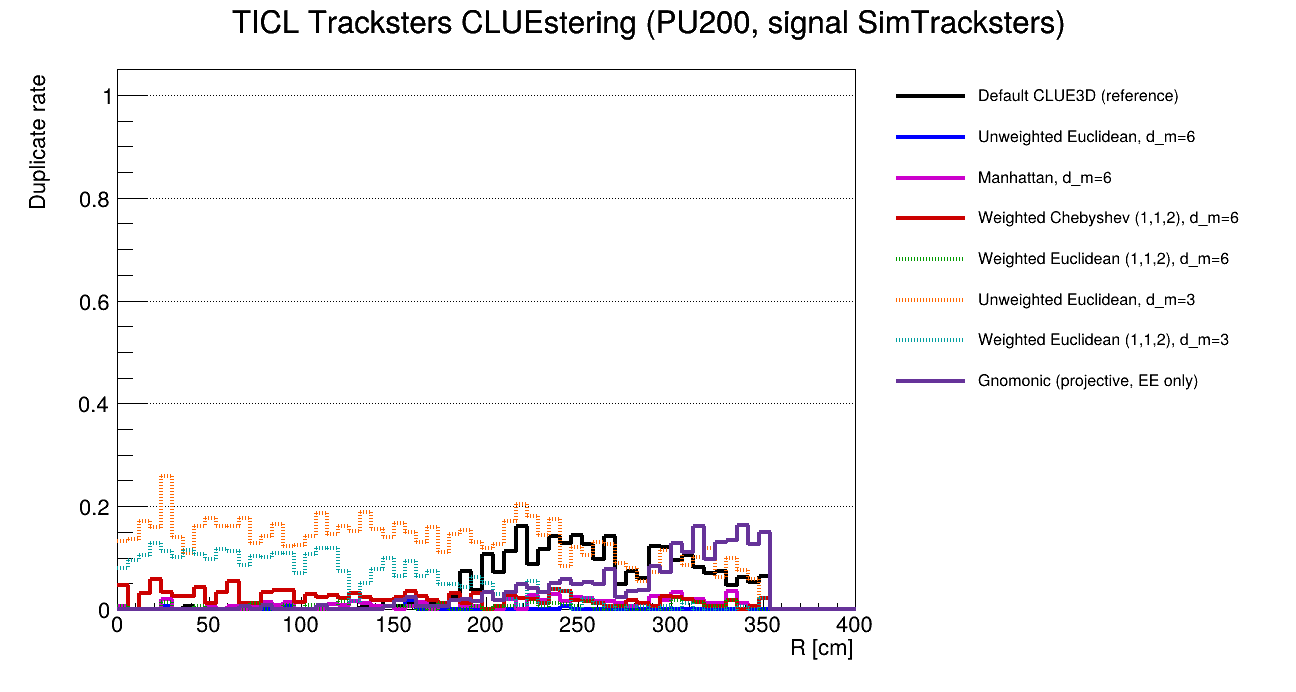
\includegraphics[width=\linewidth]{figures/cluestering_duplicates.png}
    \caption{Signal-photon duplicates versus truth displacement.}
  \end{subfigure}\hfill
  \begin{subfigure}{0.49\textwidth}
    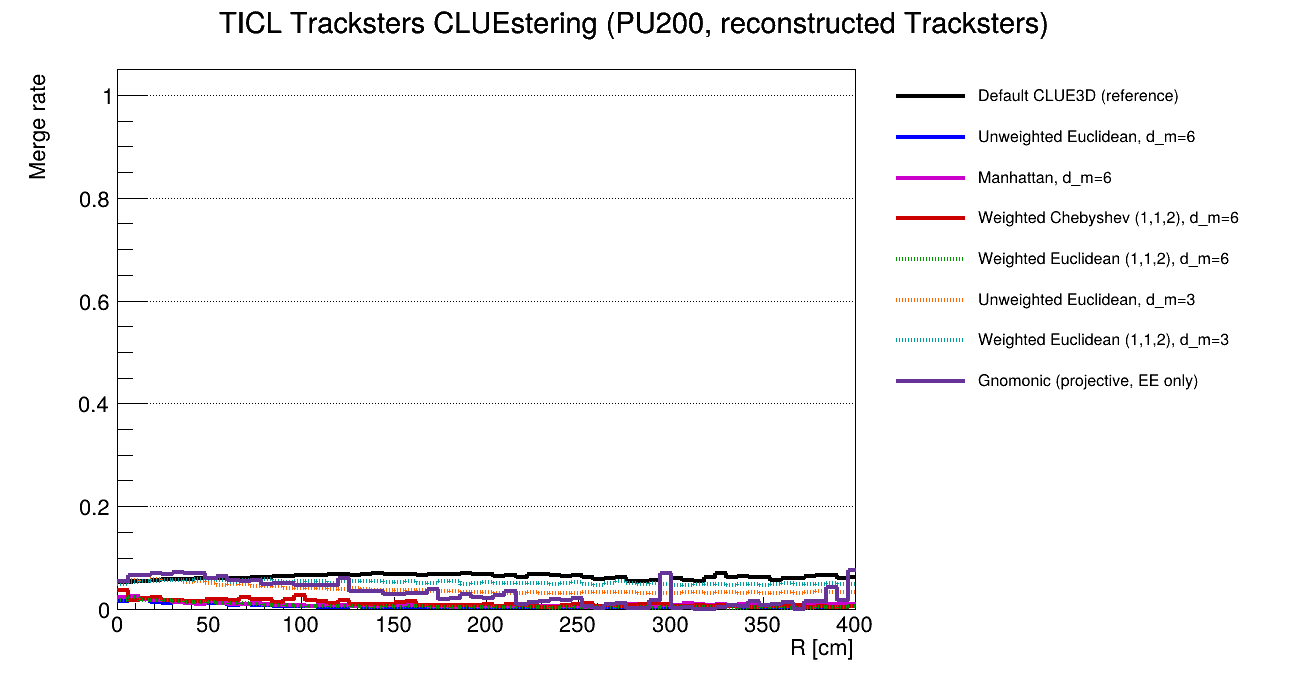
\includegraphics[width=\linewidth]{figures/cluestering_merges.png}
    \caption{Reconstructed-object merges versus barycentre radius.}
  \end{subfigure}
  \caption{Complementary PU200 rates. The duplicate denominator contains
  signal SimTracksters, while the merge denominator contains reconstructed
  Tracksters. The merge plot uses $\sqrt{x_c^2+y_c^2}$, the transverse radius
  of the Trackster barycentre, rather than its back-extrapolated displacement
  at $z=0$.}
  \label{fig:cluesteringrates}
\end{figure*}

The duplicate rates in Fig.~\ref{fig:cluesteringrates}(a) show how completely
the signal is collected into one object. The 6~cm Cartesian configurations
remain close to zero, whereas the 3~cm choices have appreciable duplicates
at small and intermediate displacement. Gnomonic duplicates rise at large
$\R$, consistent with its remaining projective fragmentation; its efficiency
gain over \cluethreed{} does not mean that every photon is recovered as one
Trackster.

The reconstructed-object merge curves in Fig.~\ref{fig:cluesteringrates}(b)
are small for the 6~cm Cartesian choices. Gnomonic and the 3~cm curves show
more merging, with gnomonic broadly comparable in size to \cluethreed{}.
These rates describe the surviving reconstructed objects, so their
interpretation must account for the very different object populations and
the efficiency loss. In particular, suppressing pileup objects can reduce
opportunities to count merges without establishing better shower separation.

\subsection{Two nearby photons and outlook}

\begin{figure*}[!tp]
  \centering
  \begin{subfigure}{0.49\textwidth}
    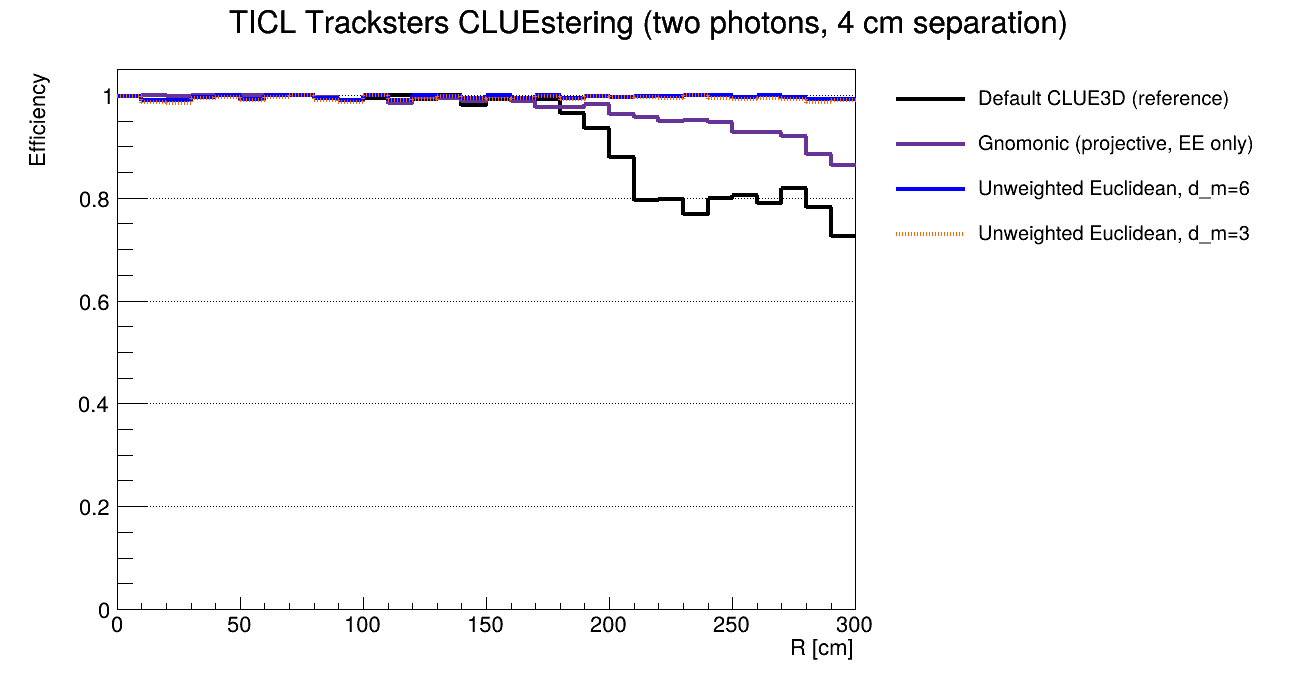
\includegraphics[width=\linewidth]{figures/cluestering_two_photon_efficiency.png}
    \caption{Photon reconstruction efficiency.}
  \end{subfigure}\hfill
  \begin{subfigure}{0.49\textwidth}
    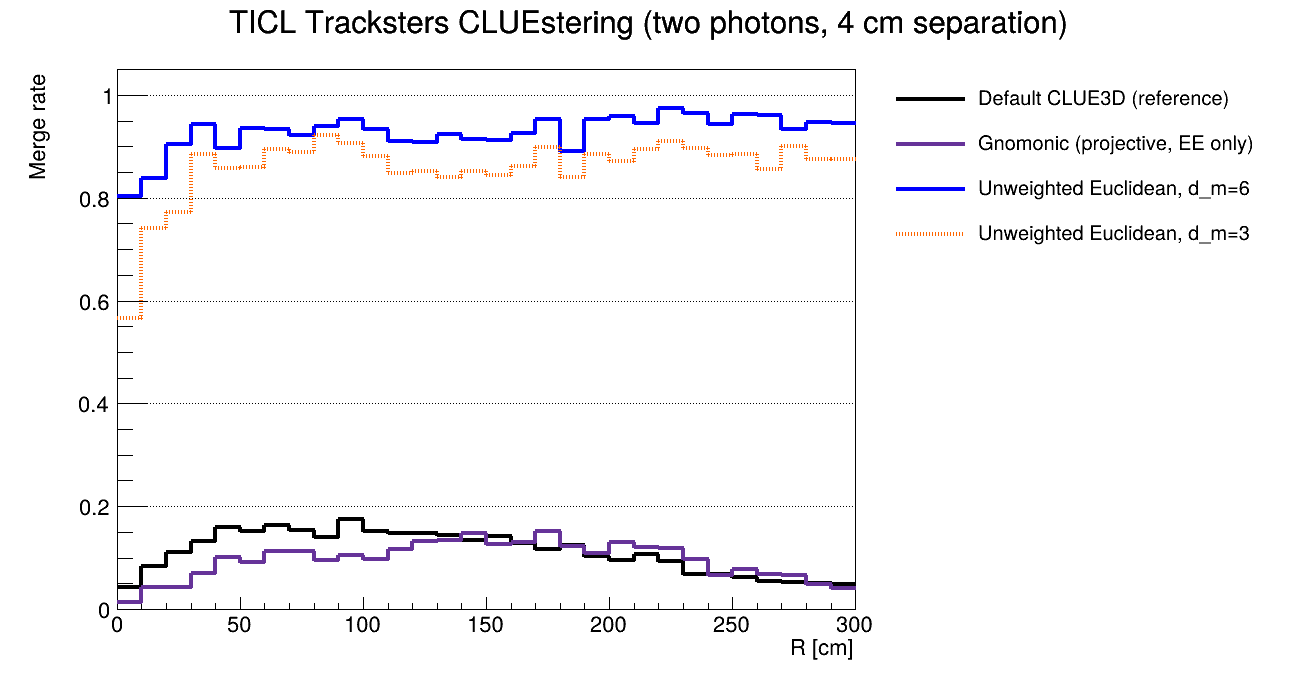
\includegraphics[width=\linewidth]{figures/cluestering_two_photon_merges.png}
    \caption{Reconstructed-object merge rate.}
  \end{subfigure}
  \caption{Two photons separated by 4~cm: photon efficiency and
  reconstructed-object merge rate for default \cluethreed{}, the gnomonic
  configuration, and unweighted Euclidean at $d_m=6$ and $3$~cm. Efficiency is
  binned in truth displacement and merge rate in reconstructed displacement,
  with 10~cm bins over 0--300~cm. The merge denominator contains nonempty
  Tracksters.}
  \label{fig:cluesteringtwophoton}
\end{figure*}

A dedicated two-photon comparison at 4~cm separation tests nearby showers
directly (Fig.~\ref{fig:cluesteringtwophoton}). Here efficiency cannot be read
on its own: two overlapping photons collected into a single object still count
as reconstructed, so a high efficiency can just as easily mean good recovery or
outright merging. It has to be read together with the merge rate. On that
basis the gnomonic configuration holds up well: at large displacement it keeps
higher efficiency than \cluethreed{} while its merge rate stays low and close
to \cluethreed{}'s. It recovers more of each photon without merging the two
together.

The Cartesian Euclidean metrics make the point in reverse. Unweighted Euclidean
at $d_m=6$~cm reaches near-perfect efficiency, but its merge rate is very high:
the wide reach simply clusters both showers into one object, which is exactly
what made it look so strong on single photons. More surprising is $d_m=3$~cm.
Its short reach fragmented a single shower earlier, yet with two photons its
efficiency climbs back to near unity while it merges almost as heavily as the
6~cm case. The likely explanation is that the neighbouring photon bridges the
gap: activity from the second shower fills the spacing that a 3~cm reach could
not span alone, reconnecting the fragments into one merged object. This would
need a dedicated study to confirm.

As shown in Section~\ref{sec:merging}, fragmentation can also hide mixing
inside an object-based merge rate, so extending the cross-shower LC-link
diagnostic to these configurations would test separation more directly. Taken
together, the results show that \cluestering{} offers several useful choices:
the gnomonic configuration improves on \cluethreed{} in both single- and
two-photon tests, while the Cartesian metrics buy their high efficiency partly
by merging and must be tuned against that. Its strong suppression of the pileup remains a limitation of the present setup. The next
step is to extend the input coverage and tune coordinates, metric weights,
distance reaches and density settings together, using signal and PU efficiency, duplicate, merge and fake rate to guide the choice.

\section{Conclusions}
\label{sec:conclusions}

This project looked at how HGCAL clustering behaves when photons no
longer point back to the interaction point, and which specific
reconstruction features cost performance. Along the way I improved the displaced-particle gun, added displacement and timing observables
to the CMSSW validation, made the association thresholds configurable, and
produced the two-dimensional performance maps used throughout. Comparing
shower-axis estimators gave an approximately \SI{10}{cm} resolution on the
back-extrapolated displacement of the most energetic Trackster. Small fragments do
much worse than this, so it should not be read as a number that describes every
reconstructed object.

A large part of the work went into explaining why default \cluethreed{} loses
single displaced photons. Because it projects everything from the origin, two points
on the same shower axis look transversely separated by roughly $R|\Delta z|/z$,
and this apparent separation grows with displacement. The loss comes in two
stages: around $R=\SI{200}{cm}$ the energy carried by fragments whose
nearest-higher link skips two layers rises and then levels off, which produces
the intermediate plateau, and at larger displacement one-layer breaks take over
and drive the final decline. Widening the seed distance from
\SI{1.8}{cm} to \SI{2.1}{cm}, with the density radius fixed, pushes the
fragmentation out to larger displacement and recovers substantially more of the
shower.

The two-photon studies make the case that energy recovery cannot be judged on
its own. For photons \SI{4}{cm} apart, the energy linked across the two showers
keeps rising with displacement even where the object-based merge rate is
falling, so fragmentation can make the merge rate look better while the mixing
underneath is getting worse. In PU200 the injected signal photon behaves much
as it does without pileup. The inclusive truth population is a different story:
its particle mix, kinematics and shower sizes all shift with resolved
displacement, and charged particles bend in the magnetic field, so its
displacement curve cannot be read as a clean scan of production radius.

Comparing metrics through \cluestering{} showed both promise and limits.
Several Cartesian configurations stay efficient on single displaced photons
across the whole scan, including in pileup, but the Euclidean ones merge the
\SI{4}{cm} photon pair heavily, so high efficiency alone does not mean the two
particles were actually resolved. The gnomonic configuration was the
most encouraging, giving higher efficiency than default \cluethreed{} at large
displacement while keeping a low merge rate on the two-photon test, though this
still needs further studies and its EE-only
coverage is why its inclusive pileup efficiency looks so low.

The natural next step is to tune coordinates, metric weights, distance scales
and density thresholds together, judging them against energy recovery,
fragmentation and cross-shower mixing at once. It also needs to be tested on more
realistic inputs: the controlled photons here are injected just before HGCAL,
so they say nothing about upstream interactions or a real LLP lifetime. The
generation and validation tools built for this study give a starting point for
that work, and the geometric picture points to the specific clustering
decisions worth changing.


\section*{Acknowledgements}
I would like to thank my supervisor, Bruno Alves, for his guidance, support,
and insightful discussions throughout this project. I am also grateful to
the CERN Summer Student Programme for the chance to work and learn here this
summer.


\bibliographystyle{unsrt}
\bibliography{refs}

\end{document}
